% !Mode:: "TeX:UTF-8"

\chapter{脑电信号采集系统设计}

当前EEG采集设备高昂的价格、较大的设备体积以及复杂的操作流程是阻碍BCI系统推广的主要原因。如何在保证高质量EEG信号采集的同时,将采集设备的成本与体积控制在可接受范围内,并尽可能简化使用的复杂度,是BCI系统发展与落地的关键。针对这一问题,本章基于ARM微控制器设计了一款名为JS-AINS-40的BCI系统,其内部包含40通道的EEG采集设备,用于采集使用者的EEG信号,并可以对不同范式的EEG信号进行分析。

\section{JS-AINS-40系统性能指标}

在非侵入式BCI系统中,基于EEG信号的BCI系统由于能够捕获人脑神经细胞群自发的、节律性的电活动,具有极高的时间分辨率和较低的使用成本而得到了最广泛的应用。EEG中蕴含的大量神经影像学信息,能够为疾病诊断、人脑功能认知以及人脑状态辨识提供有力支撑。然而,EEG作为一种低幅值,低信噪比以及低频率的生理电信号,其采集难度极高。同时,EEG信号也是一种具有空间相干性的随时间快速变化的非线性生理电信号,其采集过程需要较高的空间采样率\cite{2-1}。综上所述,EEG采集仪器应当是一种具有高灵敏度、低响应延迟,能够保留信号空间相干性并可以抑制外来噪声干扰的多导联设备\cite{2-2}。

遵循上述内容,一个合格的EEG信号采集设备应当在设计时考虑以下性能指标\cite{2-3}:

(1) 输入阻抗。EEG信号作为一种微弱的生理电信号,其幅值集中在0-200 $\mu$V之间。同时,人脑头皮与EEG电极之间通常具有极高的阻抗值。这一阻抗值还会随着受试者的生理状态波动,导电介质(脑电极膏或者生理盐水)损耗,以及人脑头皮与EEG电极之间的相对位置变化而不断浮动。这导致了EEG信号采集设备需要具备尽可能高的输入阻抗值。否则人脑头皮与EEG电极之间的阻抗变化将会对EEG信号的低频段产生极大的干扰,影响整个采集过程。

(2) 共模抑制比。采集设备通常工作在充满工频干扰信号的使用环境中。$50$ Hz工频干扰信号常常以共模噪声的形式进入采集设备,混杂进EEG信号之中。极端情况下,干扰信号的幅值大小甚至会超过EEG信号,使得EEG信号淹没在噪声之中。为了提高所采集信号的质量,减少共模噪声对采集过程带来的干扰,要求EEG采集设备具有较高的共模抑制比。通常情况下,要求EEG采集设备的共模抑制比大于$90$ dB。

(3) 频率响应范围。由于EEG信号的频率范围通常在100 Hz以内,因此采集设备在采集100 Hz以内不同幅值的信号时,应当保证信号不产生失真现象。

(4) 增益大小。由于EEG信号幅值较低的特性,其难以直接被A/D芯片正常采集。因此,需要在保证不失真的前提下对信号进行放大,以保证采集过程的有效进行。

(5) 线性误差值。脑电设备应该具有尽可能小的线性误差,以保证实际输出值和理论值之间的偏差处于可接受范围,防止测量误差对人脑辨识结果造成不利影响。


\section{JS-AINS-40系统总体设计方案}


\begin{figure}[!h]
	\centering
	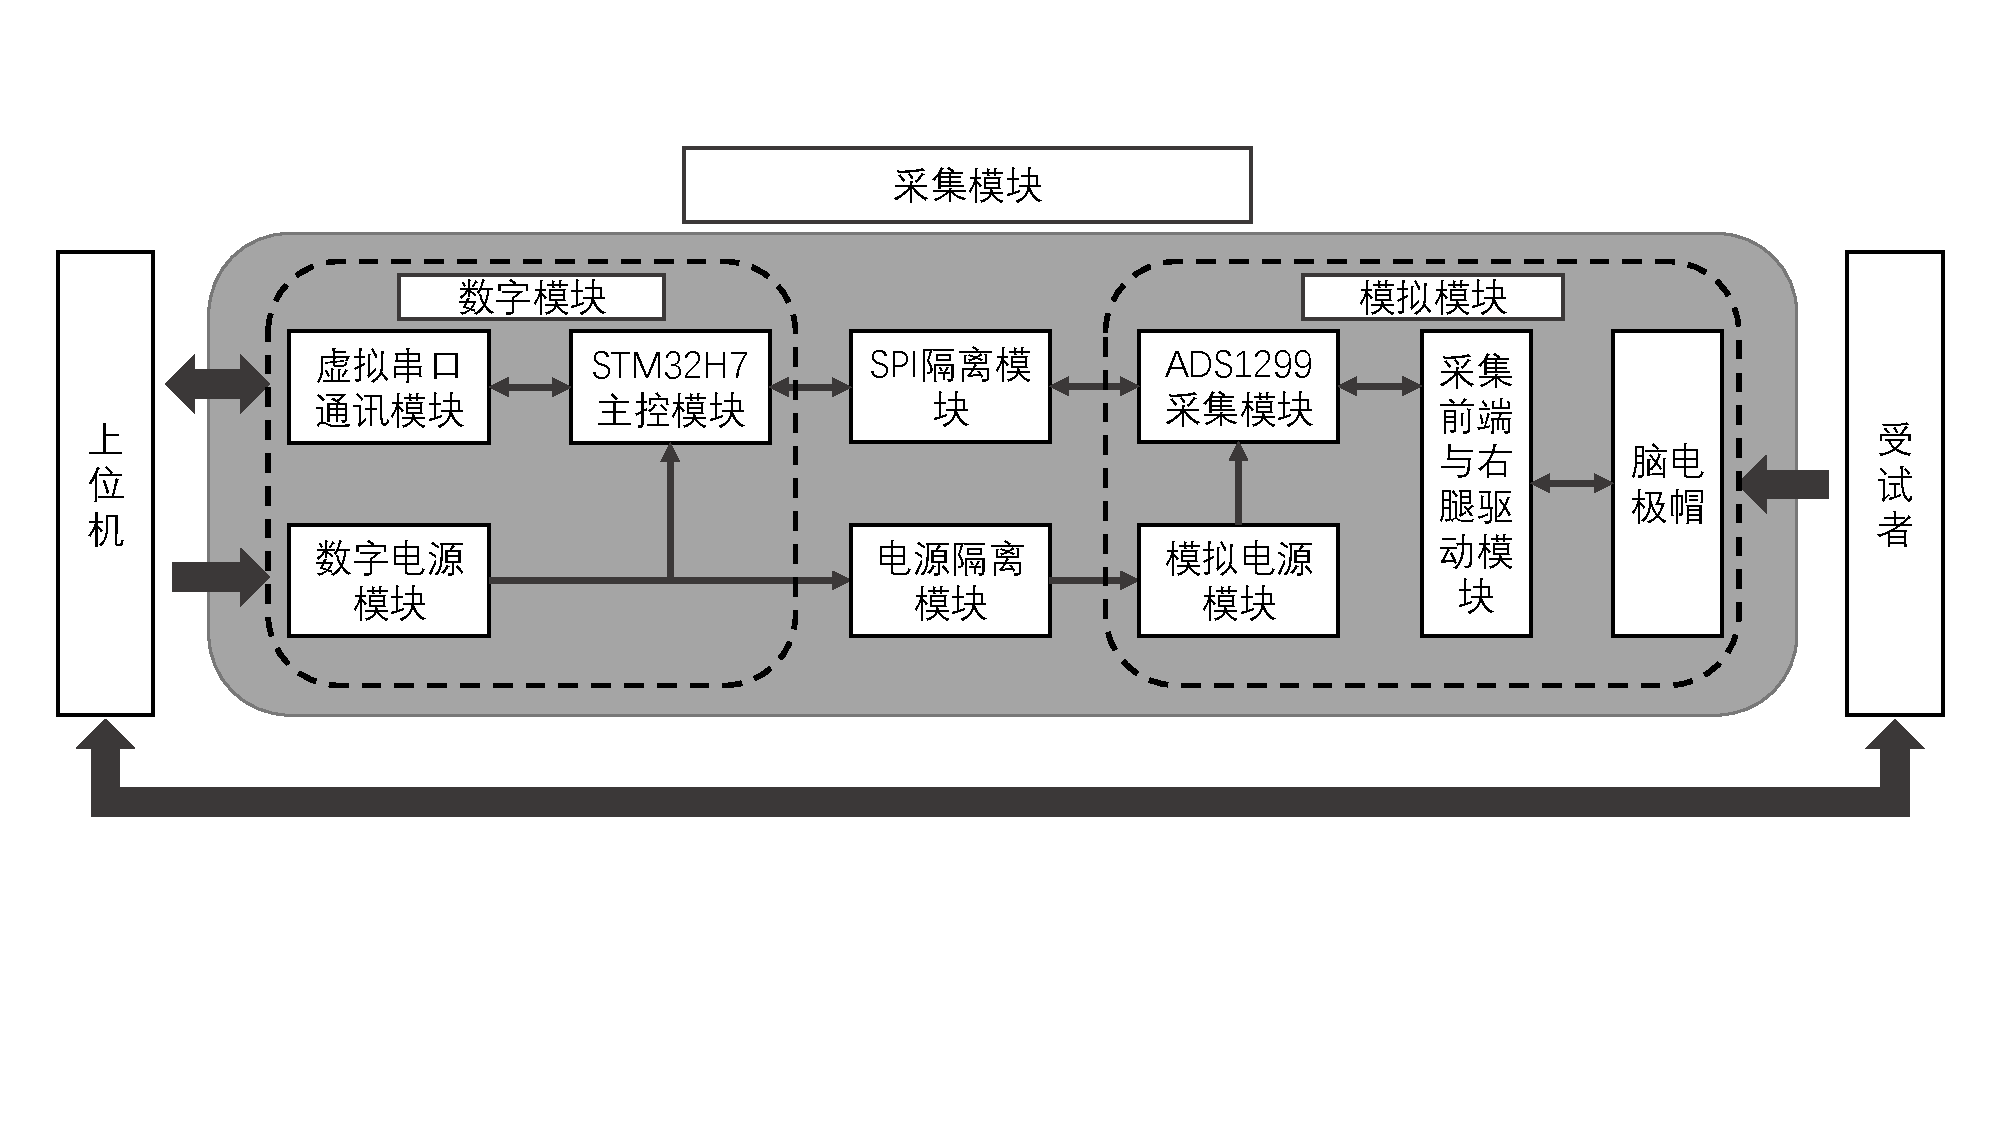
\includegraphics[width=0.60\textheight]{系统总体结构.pdf}
	\caption{JS-AINS-40系统总体结构}
	\label{fig2-1}
\end{figure}
JS-AINS-40系统的总体结构如图\ref{fig2-1}所示。其主要包含三个相互关联的不同组成部分:上位机、受试者以及中间的采集模块。其中,采集模块的设计是本节的描述重点。采集模块包括:虚拟串口通讯模块、数字电源模块、STM32H743IIT6主控模块、SPI隔离模块、电源隔离模块、ADS1299采集模块、模拟电源模块、采集前端与右腿驱动模块以及脑电极帽。其中虚拟串口通讯模块、数字电源模块与STM32H743IIT6主控模块属于数字模块。ADS1299采集模块、模拟电源模块、采集前端与右腿驱动模块以及脑电极帽属于模拟模块。

所有模块的具体工作流程如下:首先,上位机运行相应的实验程序,对受试者进行相应范式的EEG诱发。受试者产生的EEG信号被脑电极帽采集,经过采集前端与右腿驱动模块处理后以模拟信号的形式进入ADS1299采集模块。ADS1299采集模块将模拟信号转换为相应的数字信号,携带相应的设置字符串发送给STM32H743IIT6主控模块。STM32H743IIT6主控模块对数字信号进行排序与裁剪后,将处理后的数据通过虚拟串口模块发送给上位机。整个采集模块由上位机进行供电。需要注意的是,数字模块与模拟模块之间通过SPI隔离模块与电源隔离模块对信号通讯与电源传输进行隔离,防止数字模块的噪声对模拟信号采集造成影响。

\section{JS-AINS-40系统采集模块硬件结构设计}
JS-AINS-40系统的采集模块外观如图\ref{fig2-22}(a)所示。在物理结构上,其可以划分为两个组成部分,EEG采集盒和脑电极帽。
\vspace{6mm}

\begin{figure}[!h]
	\centering
	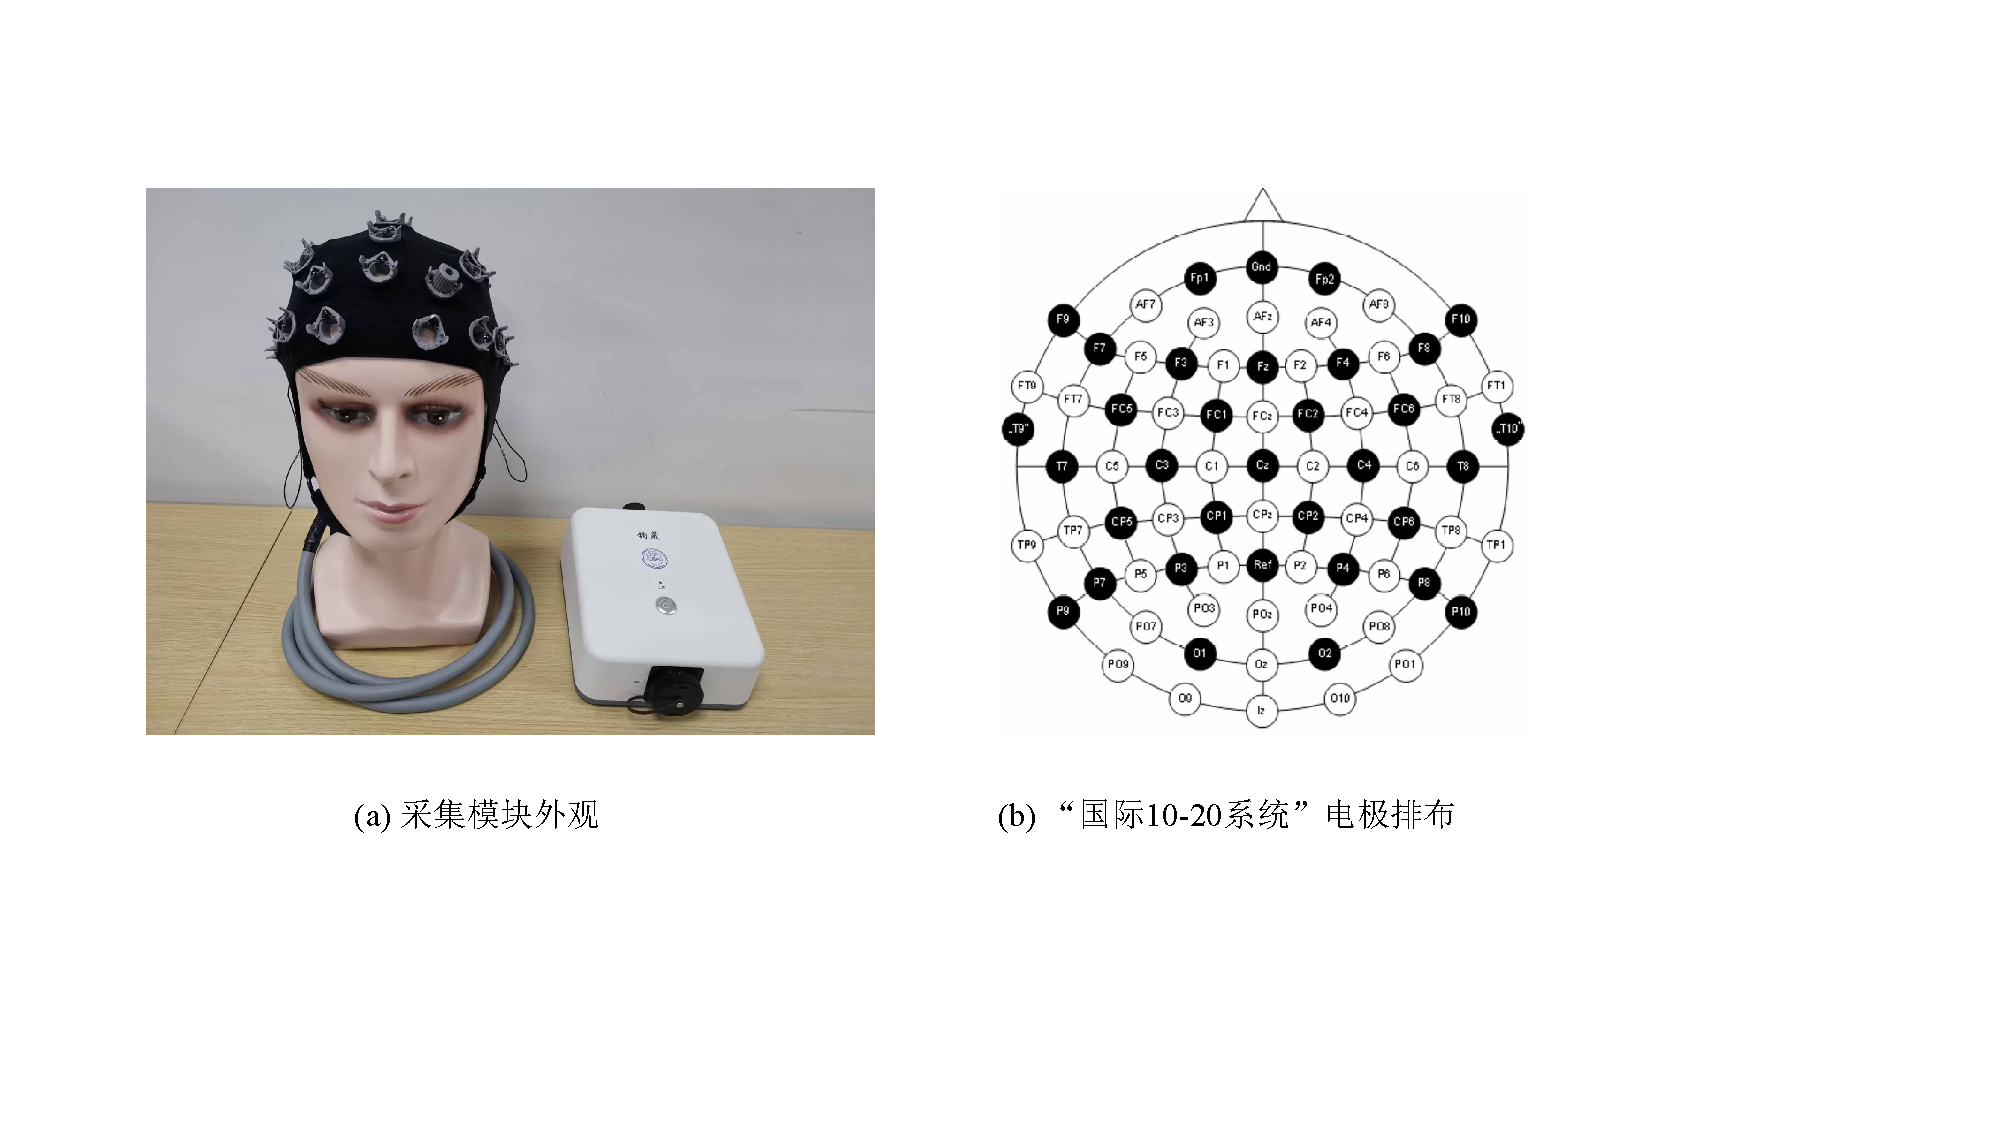
\includegraphics[width=0.6\textheight]{10-20.pdf}
	\caption{采集模块结构外观}
	\label{fig2-22}
\end{figure}

EEG采集盒体积为19.7 cm $ \times $ 15.8 cm $ \times $ 3.6 cm(长$\times$宽$\times$高),其作为采集模块的核心部件,内部包括采集模块PCB、用来固定PCB的安装立柱、LED导光柱、设备启动按钮、用来传输数据和给设备供电的USB接口以及用来连接脑电极帽的航空插头。

脑电极帽上的电极排布一般遵循“国际10-20系统”,标准的“国际10-20系统”如图\ref{fig2-22}(b)所示。自主设计的脑电极帽根据使用场景需求,选取“国际10-20系统”中的40个不同电极:FP1,FP2,AF7,AF3,AFz,AF4,AF8,F7,F3,Fz,F4,F8,FT7,FC3,FCz,FC4,FT8,T7,C3,Cz,C4,T8,TP7,CP3,CPz,CP4,TP8,P7,P3,Pz,P4,P8,PO7,PO3,POz,PO4,PO8,O1,Oz,O2,‘T9’,‘T10’。

其中‘T9’,‘T10’分别代表位于左耳后乳突的参考电极和右耳后乳突的右腿驱动电极。本设备可以同时对40个通道的EEG信号以最高1 kHz的速率进行采集,采集模块的具体设计将在后面章节详细介绍。

\section{JS-AINS-40系统采集模块硬件电路设计}

JS-AINS-40系统中的采集模块PCB实物图如图\ref{fig2-4}所示(为了方便展示,图中去除了屏蔽罩和排线),图中用不同颜色的框线标注出了各子模块的位置。在上述总体设计方案的基础上,本章详细叙述各个模块的器件选型与内部电路设计。
\begin{figure}[h!]
	\centering
	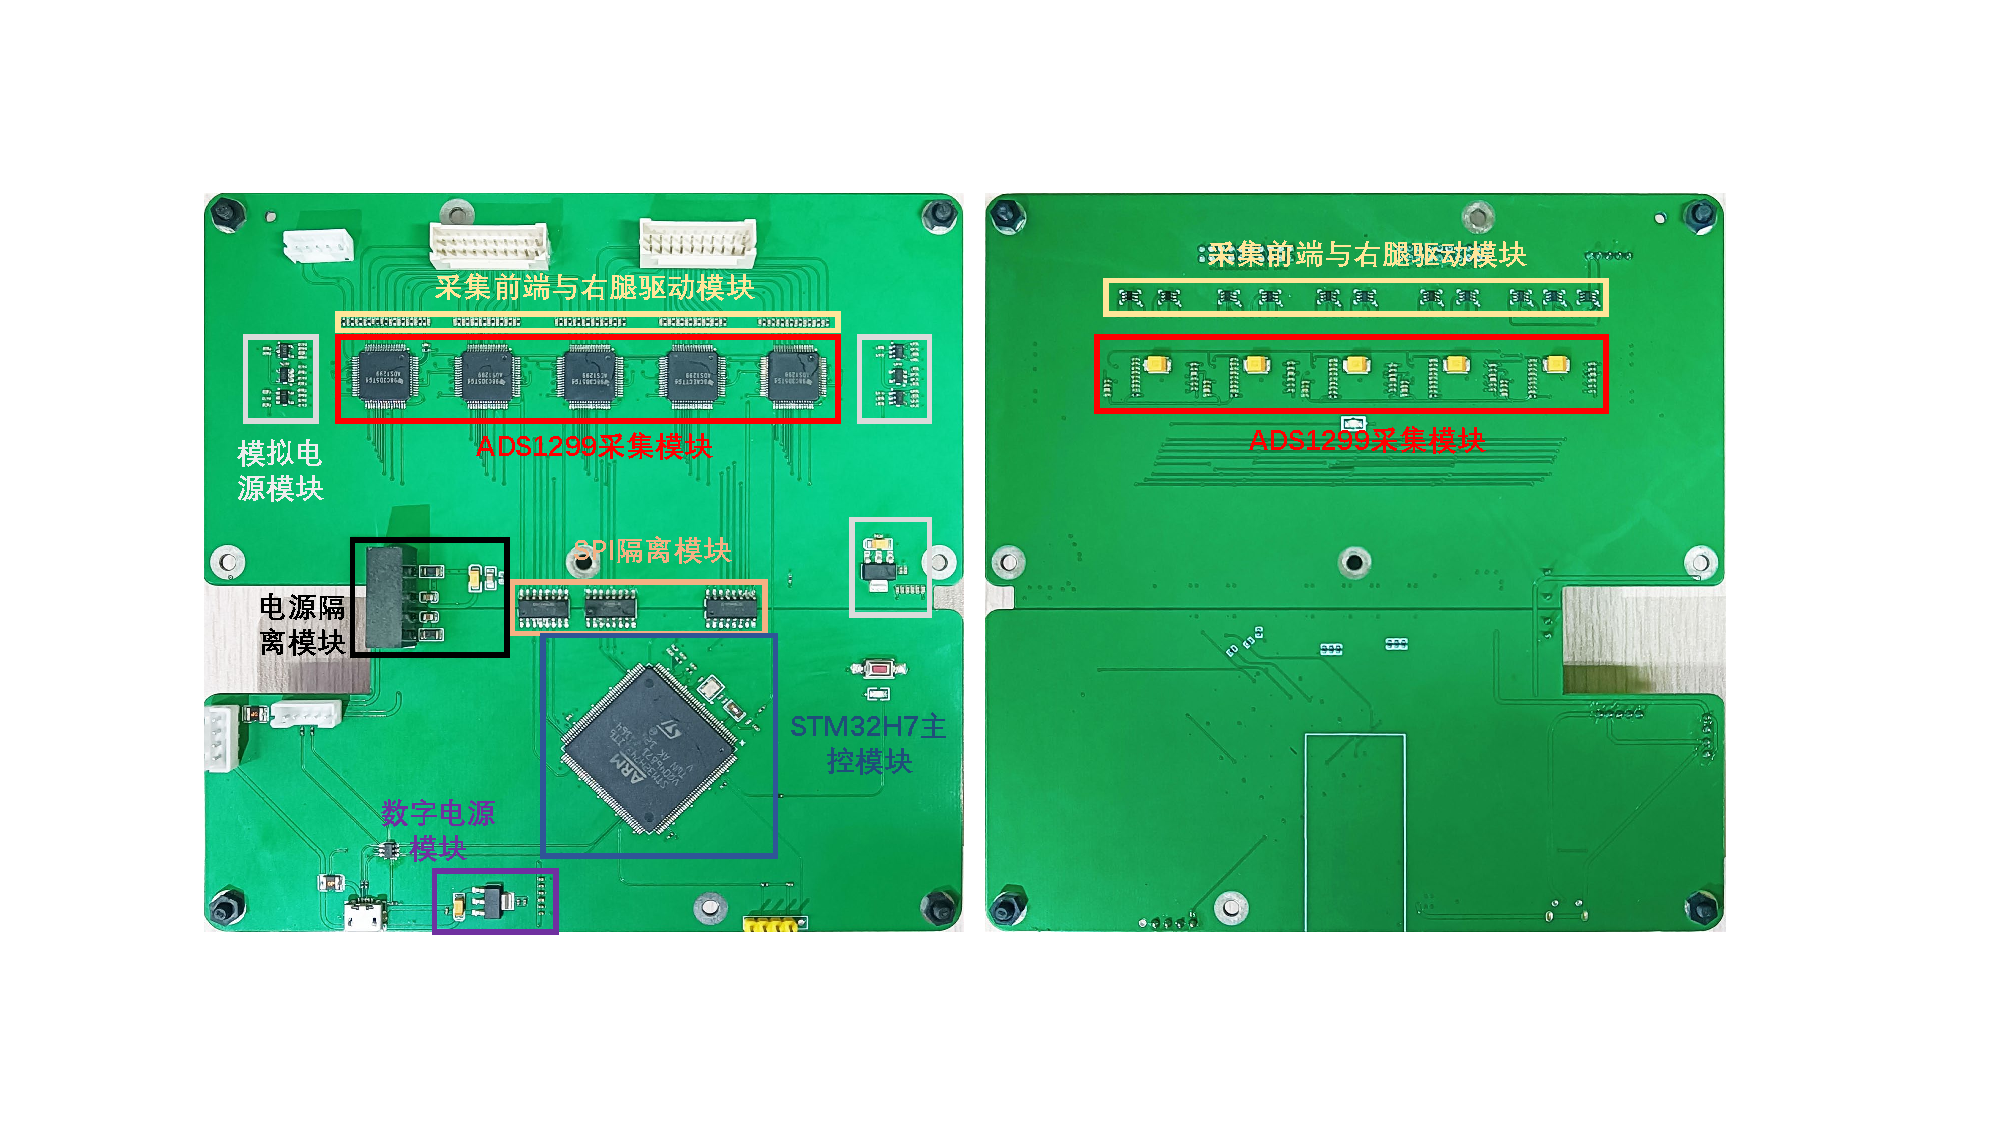
\includegraphics[width=0.50\textheight]{PCB实物图.pdf}
	\caption{JS-AINS-40系统采集模块PCB实物图}
	\label{fig2-4}
\end{figure}

毫无疑问,元器件的选型决定了设备性能的上限,而核心模块内部的芯片选型则是整个设计的重中之重,它决定了设备能否满足设计指标。因此,在开始具体的说明之前,首先对核心芯片进行介绍。采集模块中的数字模块与模拟模块分别围绕两个核心芯片构建,所有的外围模块均服务于这两个核心组件。
% \begin{figure}[!h]
% 	\centering
% 	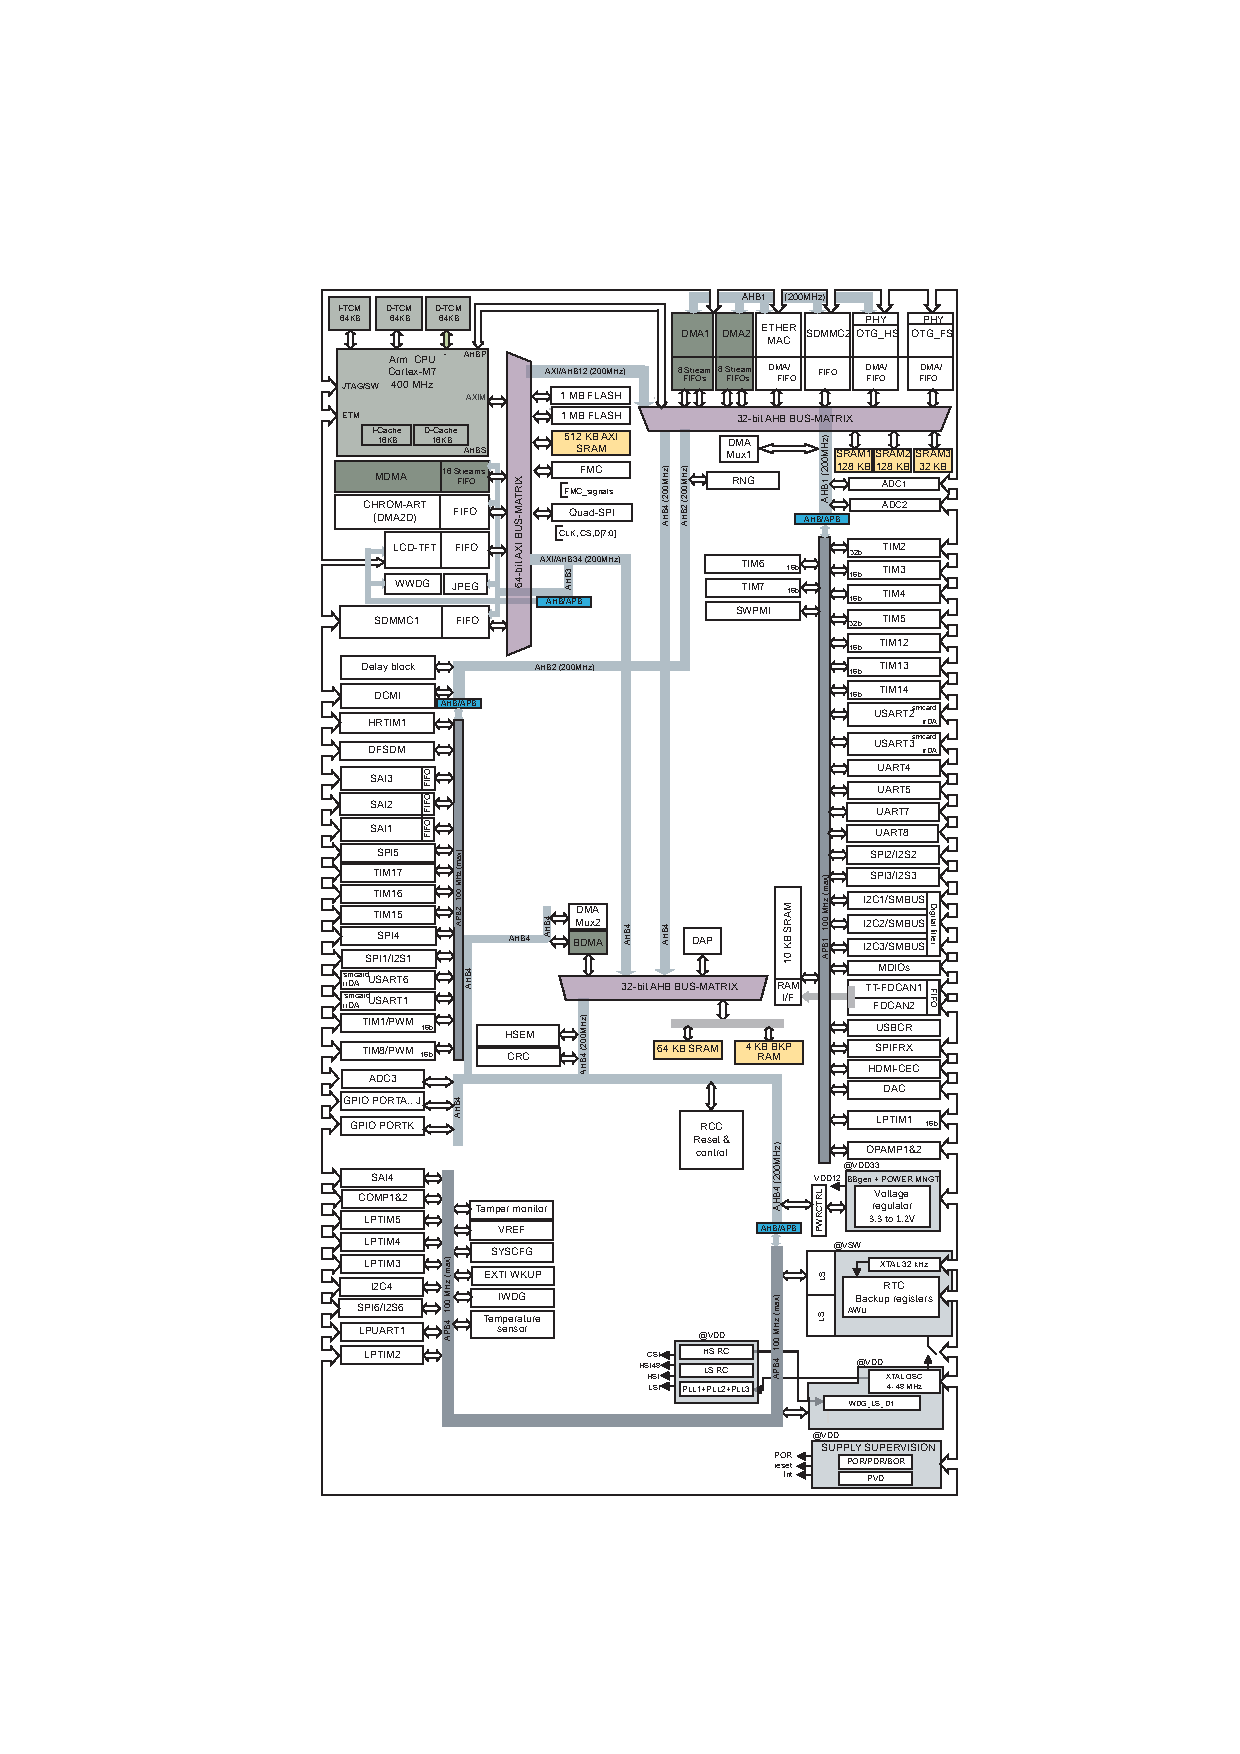
\includegraphics[width=0.44\textheight]{芯片资源_32.pdf}
% 	\caption{STM32H743IIT6内部资源展示}
% 	\label{fig2-3}
% \end{figure}
数字模块的核心选取意法半导体公司出品的STM32系列中的H743IIT6芯片。其内部的32位ARM Cortex-M7内核具有双精度FPU以及L1高速缓存(16 KB的数据缓存和16 KB的指令缓存),主频达到480 MHz,能够为40导联EEG采集设备提供所需的高速数据处理。同时,该芯片包含2 MB的闪存,1 MB RAM,168个高速(133 MHz)I/O口,4个DMA控制器,22个定时器以及大量的通讯与模拟外设。这些设备能够为40通道EEG数据提供足够的存储空间,满足主控芯片同时与多块采集芯片进行通信的需求。%STM32H743IIT6内部结构如图\ref{fig2-3}所示。
\begin{figure}[!h]
	\centering
	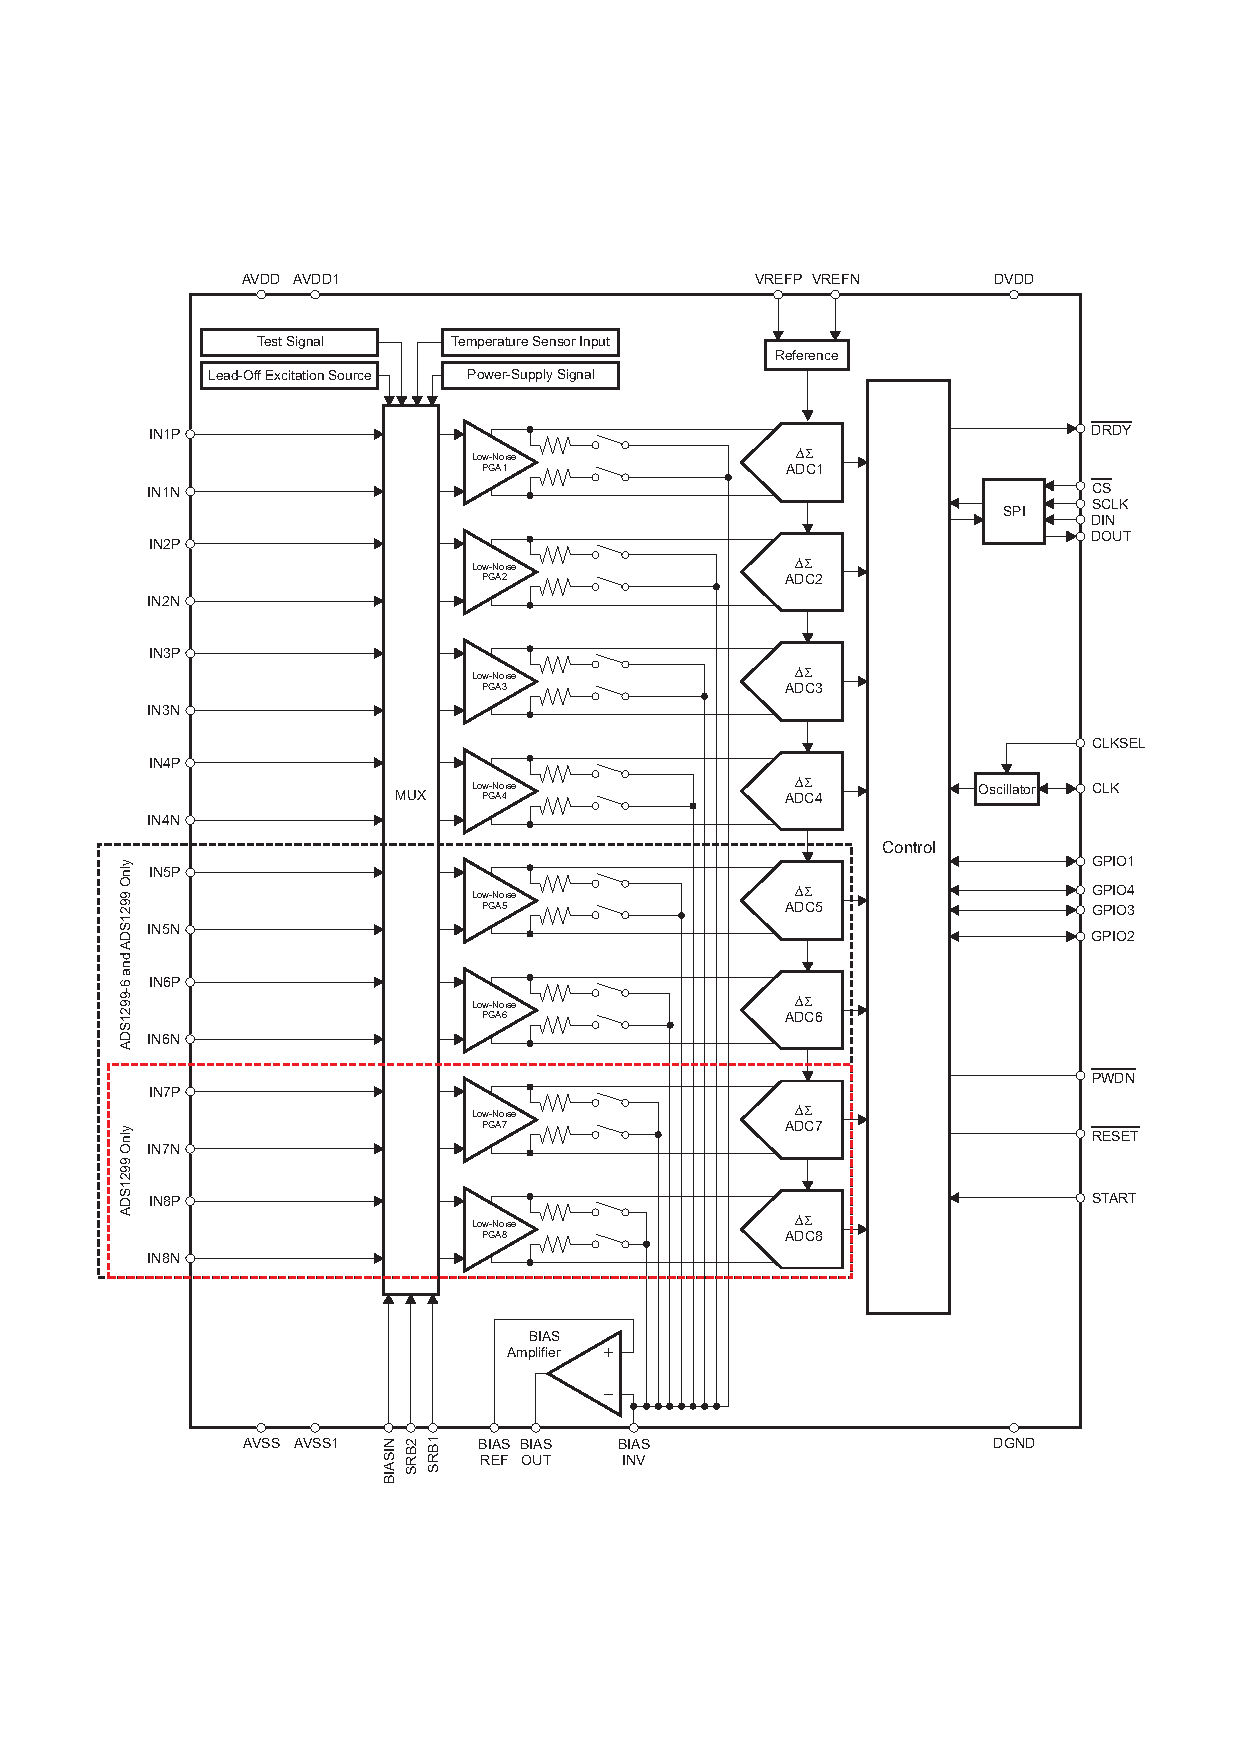
\includegraphics[width=0.50\textheight]{芯片资源_1299.pdf}
	\caption{ADS1299内部结构示意图}
	\label{fig2-2}
\end{figure}

模拟模块的核心是德州仪器公司设计的低噪声生物电势测量芯片——ADS1299。作为一款专用的8通道24位模数转换器,其内部结构如图\ref{fig2-2}所示。ADS1299内部的八个通道能够实现高分辨率下的24位同步采样,并且每个通道还配套了对应的可编程增益放大器(Programmable Gain Amplifier,PGA)。该芯片能够在任意输入通道生成患者的偏置输出信号(右腿驱动功能),并自主选取反馈连接方式。此外,该芯片还能够在–40$^{\circ}$C至+85$^{\circ}$C的工作环境下,以250 Hz至16 kHz的采样率完成EEG信号采集工作,完全满足当前EEG采集任务的要求。ADS1299作为一款成熟的EEG采集芯片,其设计高度集成化,性能可靠且能够满足EEG采集设备的设计指标,因此本章以其作为模拟模块的核心。

\subsection{电源模块设计}

电源模块为整个系统提供能源保障,是系统能够正常工作的“根基”。电源模块在设计时需要充分考量设备的具体能耗,并留出充足的裕量以应对特殊情况。如果电源的参数选取不合理,轻则导致设备无法长时间稳定工作,重则造成设备损毁,危及使用者安全。兼顾设备性能与元器件成本的电源设计,将是整个系统设计的基础。JS-AINS-40系统采集模块的电源包括数字电源模块与模拟电源模块。

采集模块使用上位机PC端的USB端口为整个模块供能,大幅简化了设备使用条件。但与此同时,PC端因为直接接入220 V市电电网,毫无疑问会具有较大的噪声干扰。尽管这些干扰不会影响PC的正常运行,但对于采集微弱EEG信号的采集模块,这些噪声的存在将会是毁灭性的。因此,本章在设计时将数字电源模块与模拟电源模块进行隔离。

(1) 数字电源模块设计

数字电源模块为采集模块中的虚拟串口通讯模块、STM32H743IIT6主控模块和SPI隔离模块的数字侧供能。上述模块均工作在直流3.3 V电压下,而USB端口只能提供直流5 V供电,因此需要数字电源模块进行电压转换。同时,考虑到数字模块对噪声具有较强的鲁棒性,本节选取德州仪器生产的TLV1117-33CDCYR芯片将PC的5 V供电转换为3.3 V,并直接提供给数字模块使用。实验证明,这一设计符合性能需求。TLV1117-33CDCYR是一款正输出低压差线性稳压器(Low-Dropout Regulator,LDO),能够为负载提供800 mA的电流输出。该LDO在输入电压与输出电压压差达到1.2 V以上时即可正常工作、具有较好的纹波表现,并且仅需设计简单的外围电路。上述优点促使本节选取其作为数字模块供电芯片。图\ref{fig2-5}展示了TLV1117-33CDCYR的原理图。

\begin{figure}[!h]
	\centering
	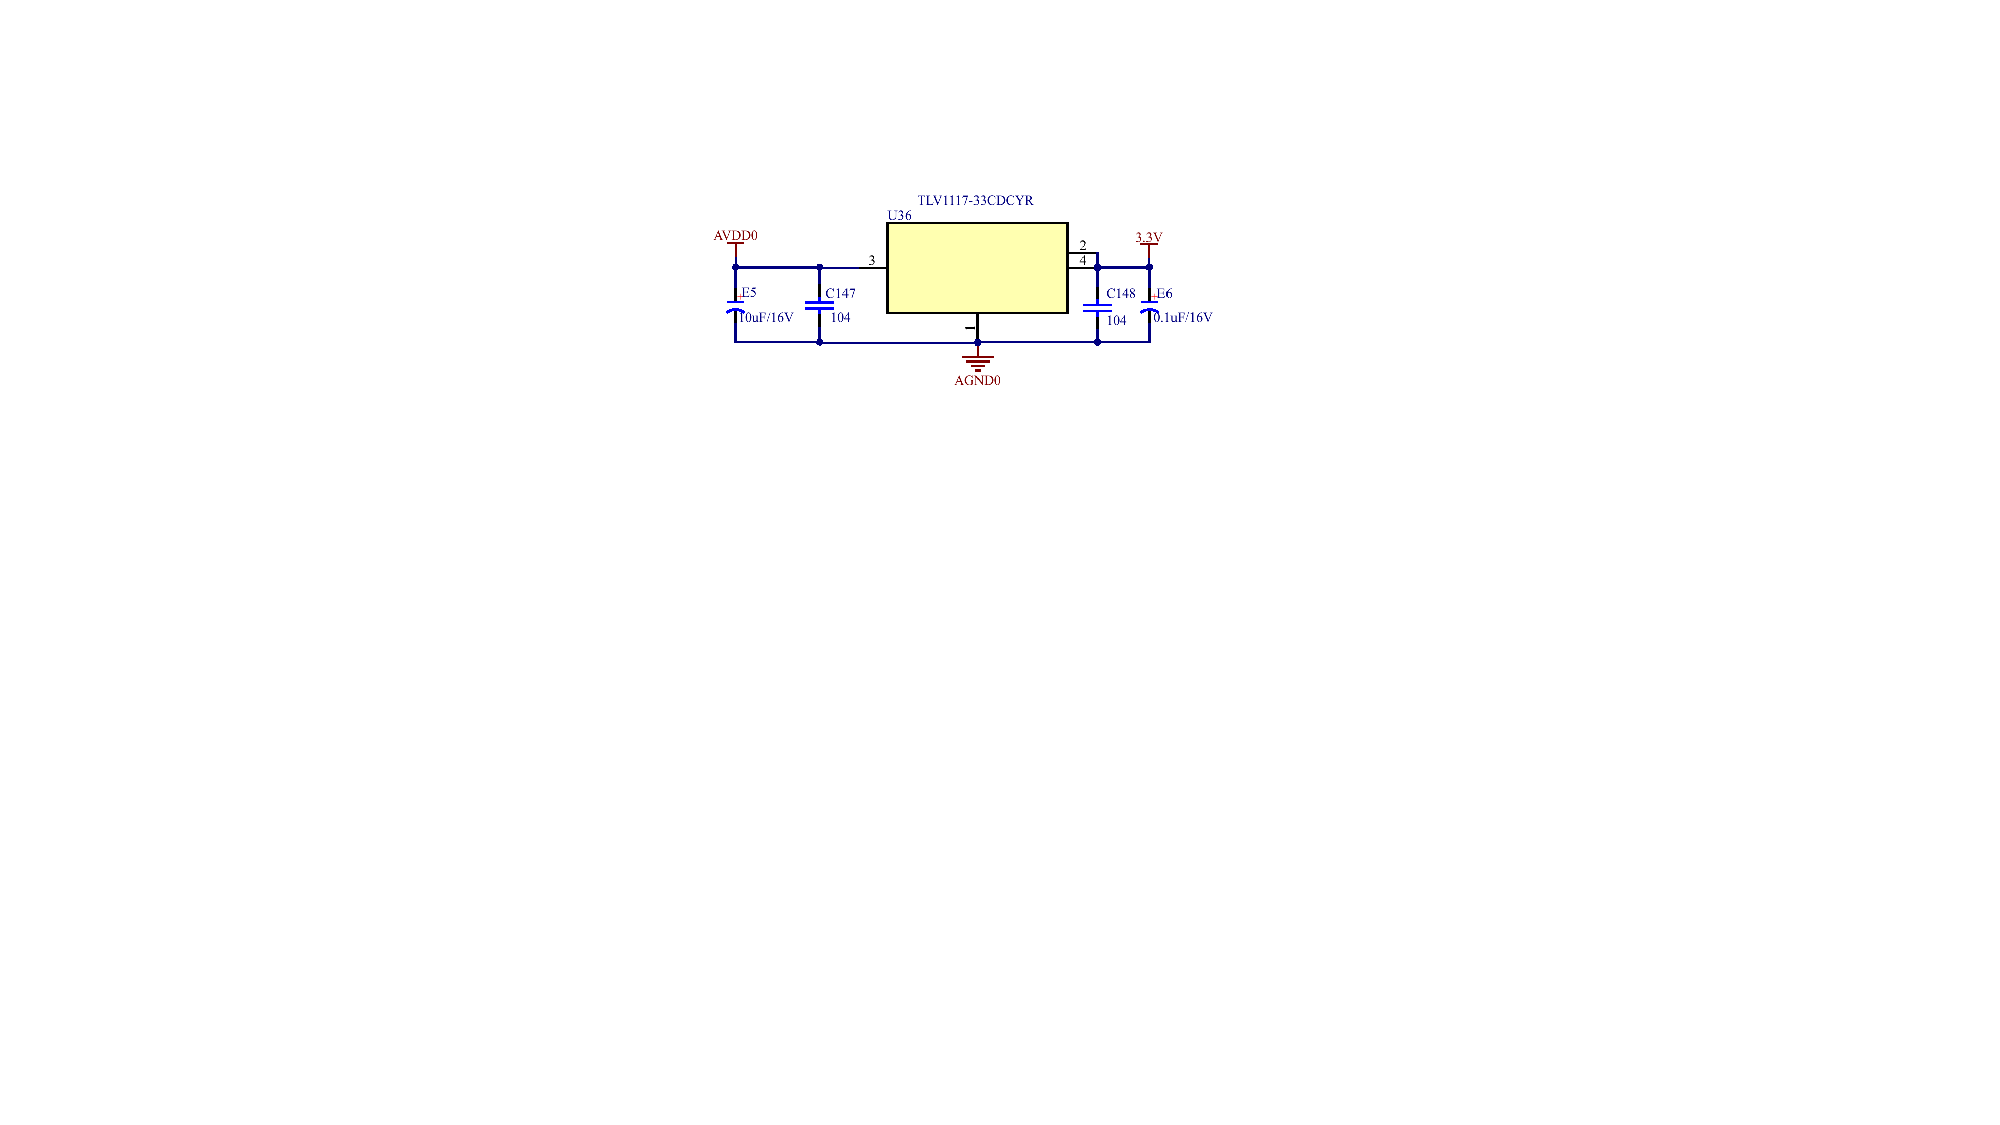
\includegraphics[width=0.46\textheight]{数字1117.pdf}
	\caption{TLV1117-33CDCRY原理图}
	\label{fig2-5}
\end{figure}

(2) 电源隔离模块设计

\begin{figure}[!h]
	\centering
	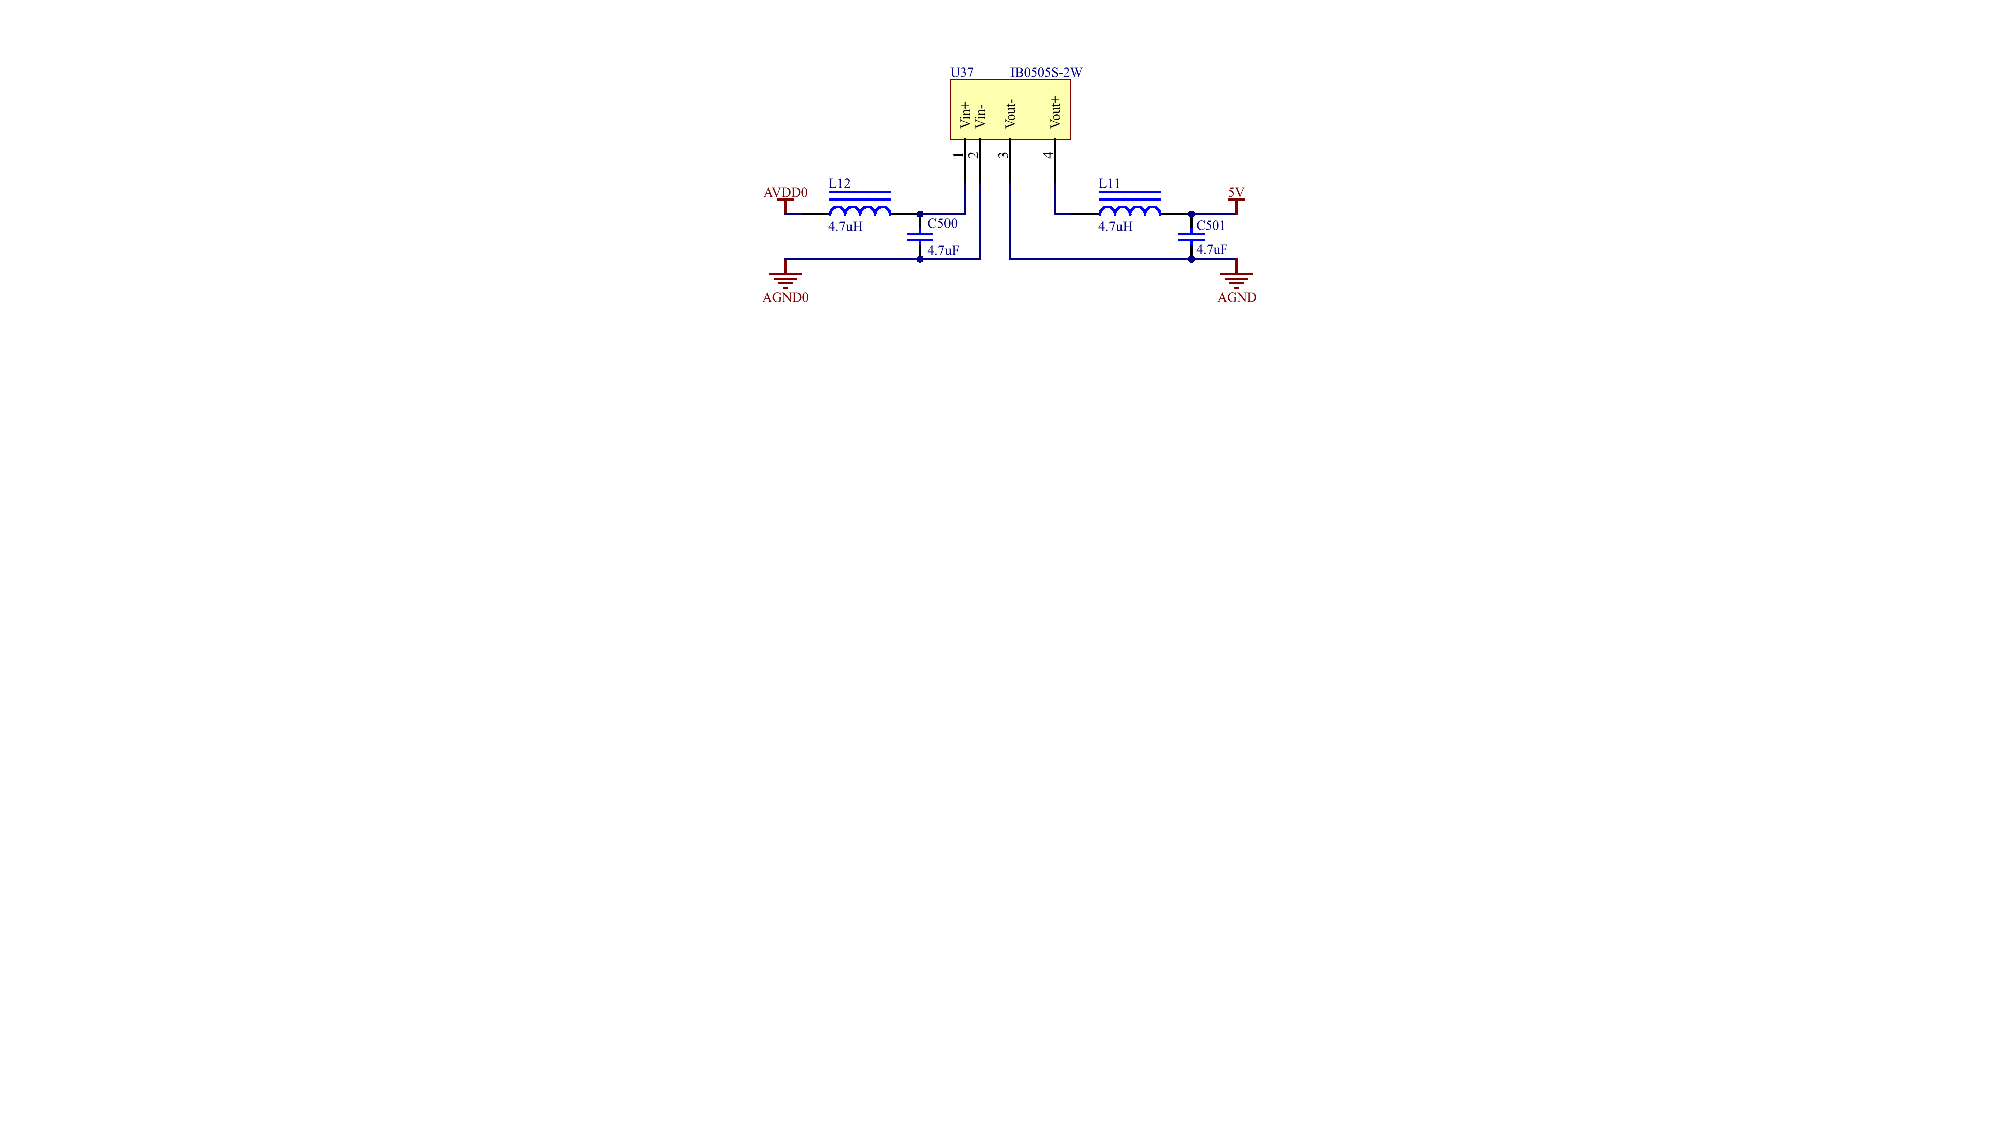
\includegraphics[width=0.46\textheight]{DCDC.pdf}
	\caption{IB0505S-2W原理图}
	\label{fig2-6}
\end{figure}

为了提升JS-AINS-40系统的安全性,并隔离数字端可能存在的噪声干扰,在数字电源模块与模拟电源模块之间添加电源隔离模块。综合考虑使用场景,引入金升阳公司的DCDC模块电源IB0505S-2W进行电源隔离。其具备较小的体积、与ADS1299相近的适用温度、良好的温度特性、1000 VDC的隔离能力、最大2 W的输出功率以及80\%的转换效率,满足模拟模块的使用要求。本节将USB端口的5 V供电输入IB0505S-2W,其输出的5 V电压作为模拟模块的电源。IB0505S-2W的相关电路如图\ref{fig2-6}所示。

(3) 模拟电源模块设计

模拟电源模块为ADS1299采集模块、SPI隔离模块的模拟侧以及采集前端与右腿驱动模块供电。根据ADS1299的设计需求,本章选择双极电源为其供电。分别为ADS1299的AVDD引脚提供$\rm +2.5$ V的模拟正电源,AVSS引脚提供$\rm -2.5$ V的模拟负电源以及DVDD引脚提供3.3 V的模拟电源。由于本章设计使用ADS1299的内部参考电压,而内部参考电压基于AVSS生成。内部参考电压$\mathrm{~V}_{\mathrm{REF}}$的大小直接影响了ADS1299信号幅值测量的准确性:

\begin{equation}
    \label{deqn_ex2_1}
\text{量程范围} =\frac{\pm \mathrm{V}_{\mathrm{REF}}}{\text { Gain }}=\frac{2 \mathrm{~V}_{\mathrm{REF}}}{\text { Gain }}
\end{equation}
其中$\text{Gain}$为ADS1299的内部PGA增益。因此,模拟电源模块的供电芯片,特别是AVSS引脚的$\rm -2.5$ V供电芯片需要专门挑选低纹波线性稳压器。

本节设计的具体选型如下:将电源隔离模块IB0505S-2W输出的5 V供电作为电源,分别传递给TLV1117-33CDCRY、TPS60403DBVR和TPS73225DBVR。TLV1117-33CDCRY已经在数字电源模块使用过一次,不再详细介绍。其输出的3.3 V为ADS1299的DVDD供电。TPS60403DBVR是德州仪器公司生产的一款电荷泵电压逆变器,其能够以90\%的效率将输入转化为负输出电压,并为负载提供60 mA的电流。本节中,使用TPS60403DBVR将5 V转化为-5 V,提供给TPS72325DBVR。TPS72325DBVR是德州仪器公司生产的低噪声、高电源抑制比的负输出线性稳压器。其输出噪声低于60 $\mu V_{RMS}$,电源抑制比在$1$ kHz时为$65$ dB,内部提供短路与过载检测保护装置,符合当前的设计要求。因此,本节使用TPS72325DBVR将-5 V转化为-2.5 V作为输入传递给ADS1299的AVSS。TPS73225DBVR同样来自德州仪器公司,是一款低噪声线性稳压器。其输出噪声低于30 $\mu V_{RMS}$,电源抑制比在$1$ kHz时为$55$ dB,内部提供反向电流保护装置,符合当前的设计要求。本节使用TPS73225DBVR将5 V转化为2.5 V提供给ADS1299的AVDD。为保证设备可靠运行,设计两组相同的供电电路分别为一半数量的ADS1299供能,两组电源能够提供的功率为600 mW,远高于模拟模块所需总功率。整个设计如图\ref{fig2-7}所示。

\begin{figure}[h]
	\centering
	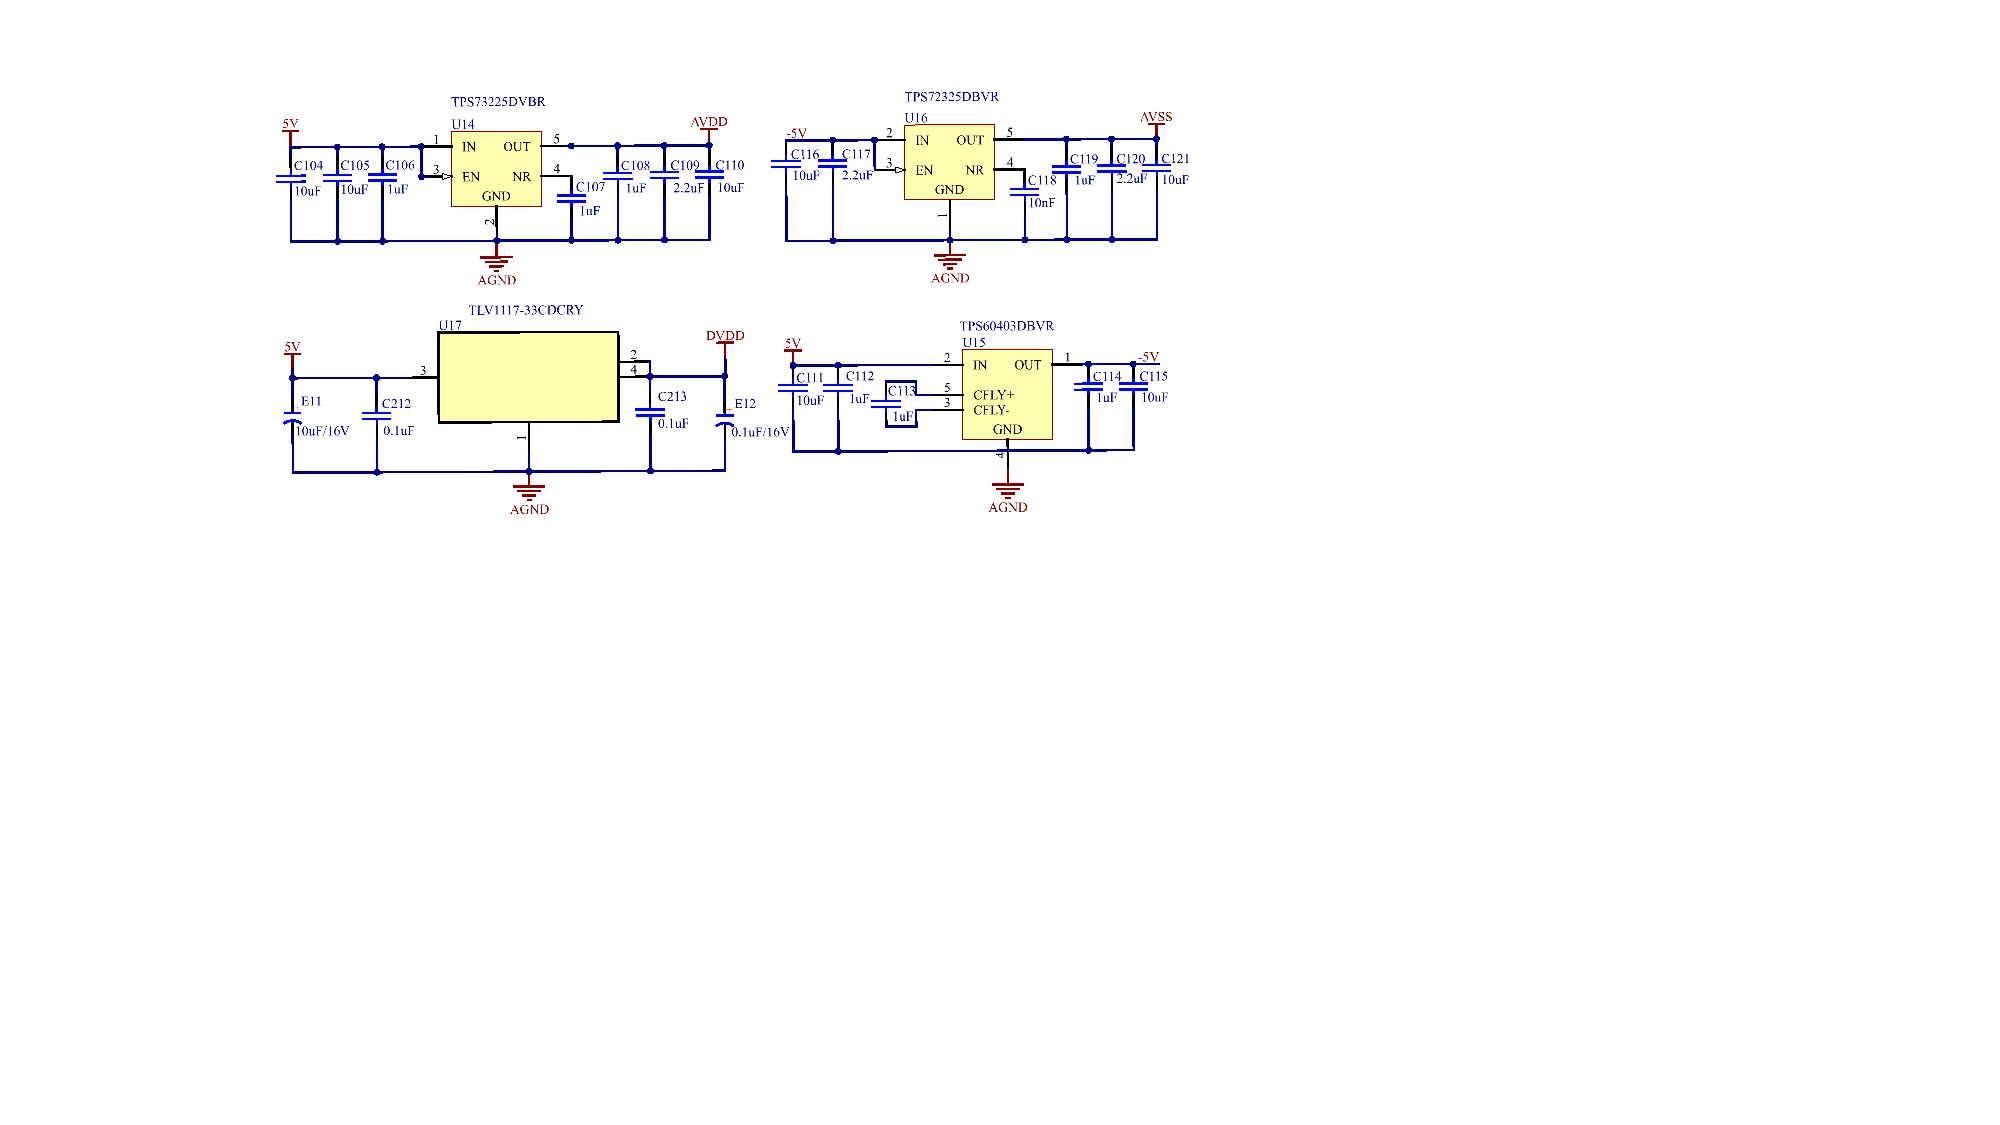
\includegraphics[width=0.62\textheight]{模拟电源模块.pdf}
	\caption{模拟电源模块原理图}
	\label{fig2-7}
\end{figure}

\subsection{STM32H743IIT6主控模块设计}
\begin{figure}[!h]
	\centering
	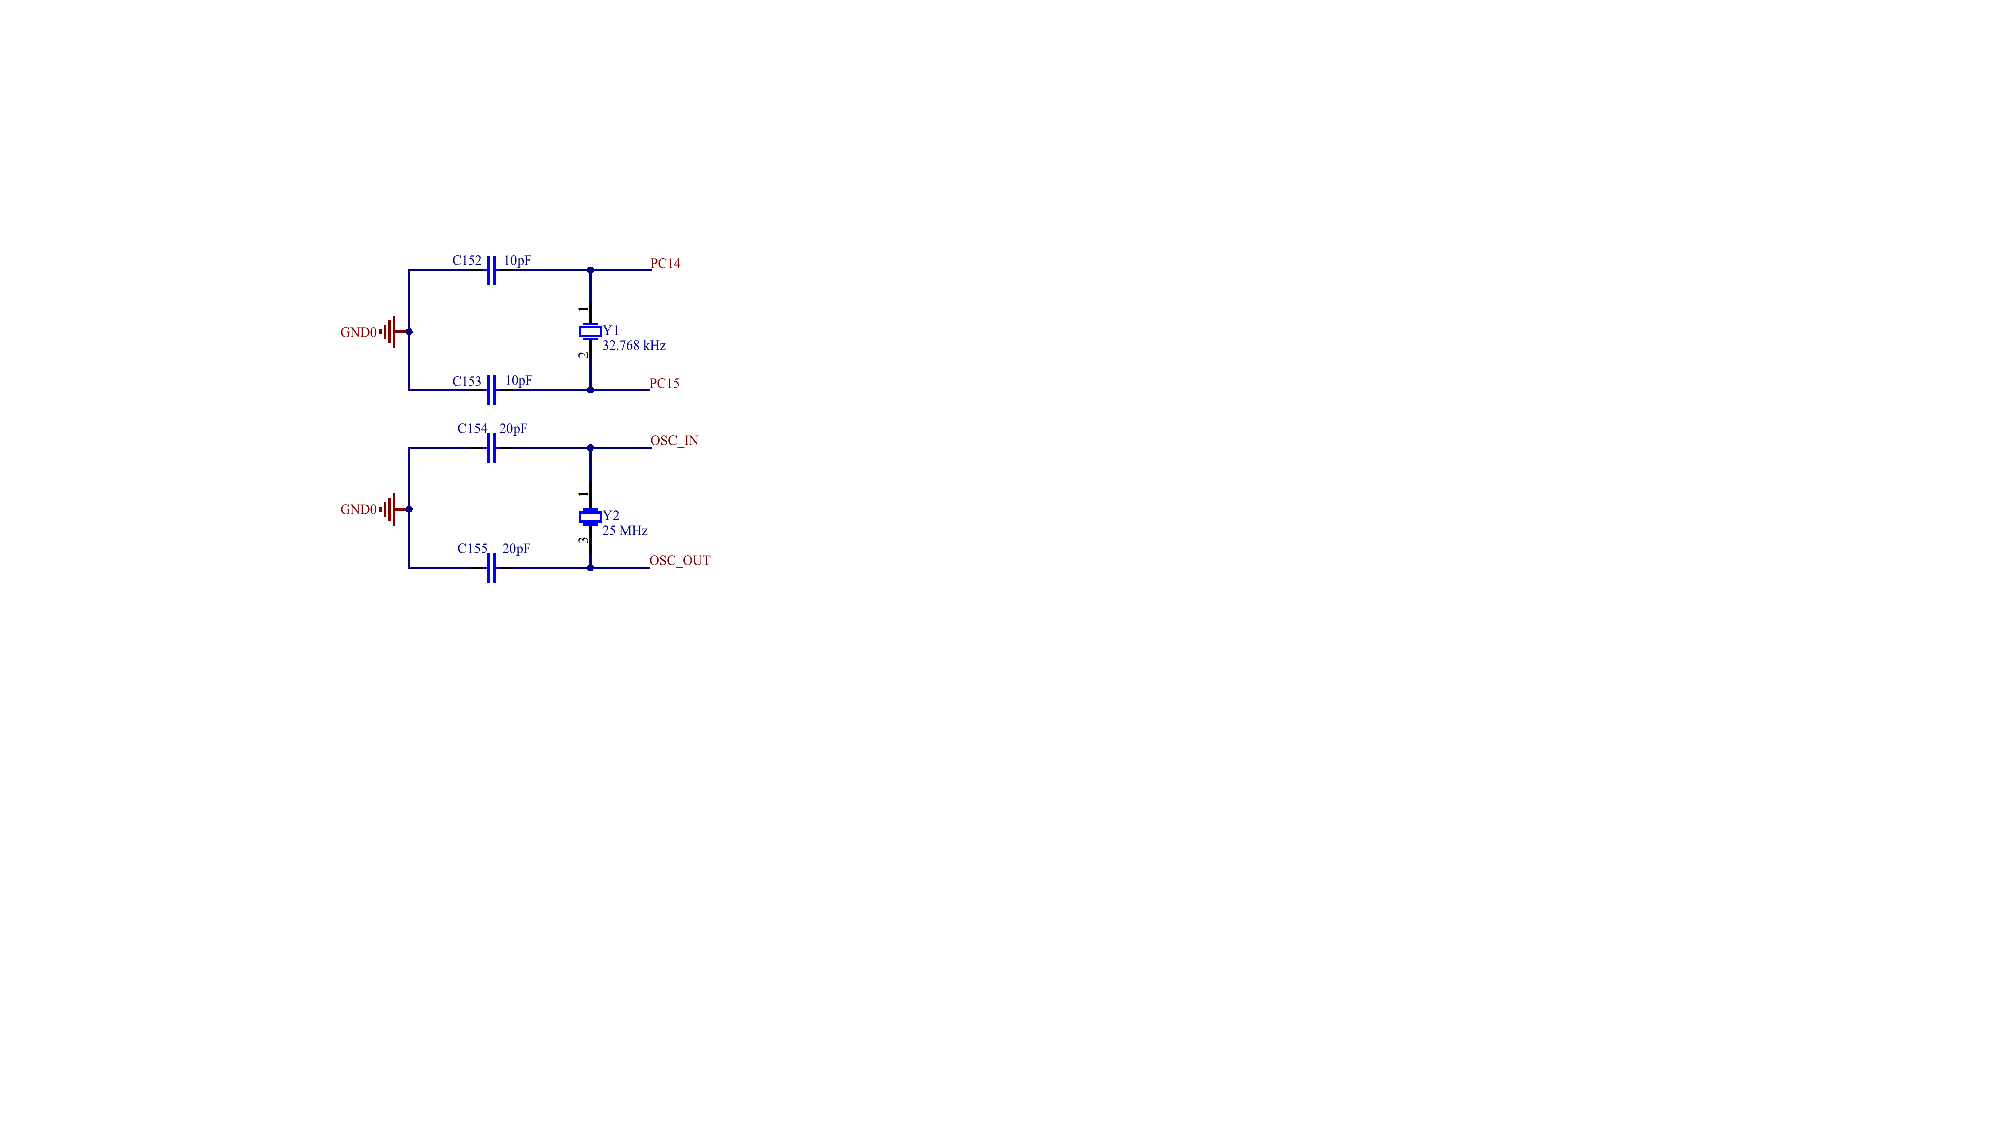
\includegraphics[width=0.32\textheight]{时钟电路.pdf}
	\caption{时钟电路原理图}
	\label{fig2-8}
\end{figure}

JS-AINS-40系统的主控模块围绕STM32H743IIT6芯片搭建。主控模块负责:配置ADS1299设置寄存器,使其以期望模式采样EEG数据;接收、切割、存储ADS1299回传的数据;将处理后的回传数据通过虚拟串口通信模块转发给上位机。

为了保证主控模块正常工作,给STM32H743IIT6芯片搭建了配套的时钟电路、复位电路和调试电路。其原理图如图\ref{fig2-8}所示。根据STM32H743IIT6的芯片手册,使用爱普生公司的X1E0000210621 25 MHz晶振和Q13FC1350000400 32.768 kHz晶振设计时钟电路,分别作为高速时钟源和低速时钟源。外部高速时钟源通过PLL锁相环电路倍频至400 MHz,维持系统内核时钟稳定。外部低速时钟源保证看门狗和实时时钟(Real Time Clock,RTC)不受其他因素干扰。


复位电路能够保证每次上电开机后,主控模块自动复位,同时能够在必要时通过手动复位芯片。其原理图如图\ref{fig2-9}所示,开机时或按键后,STM32的RESET引脚将被拉低。

\begin{figure}[!h]
	\centering
	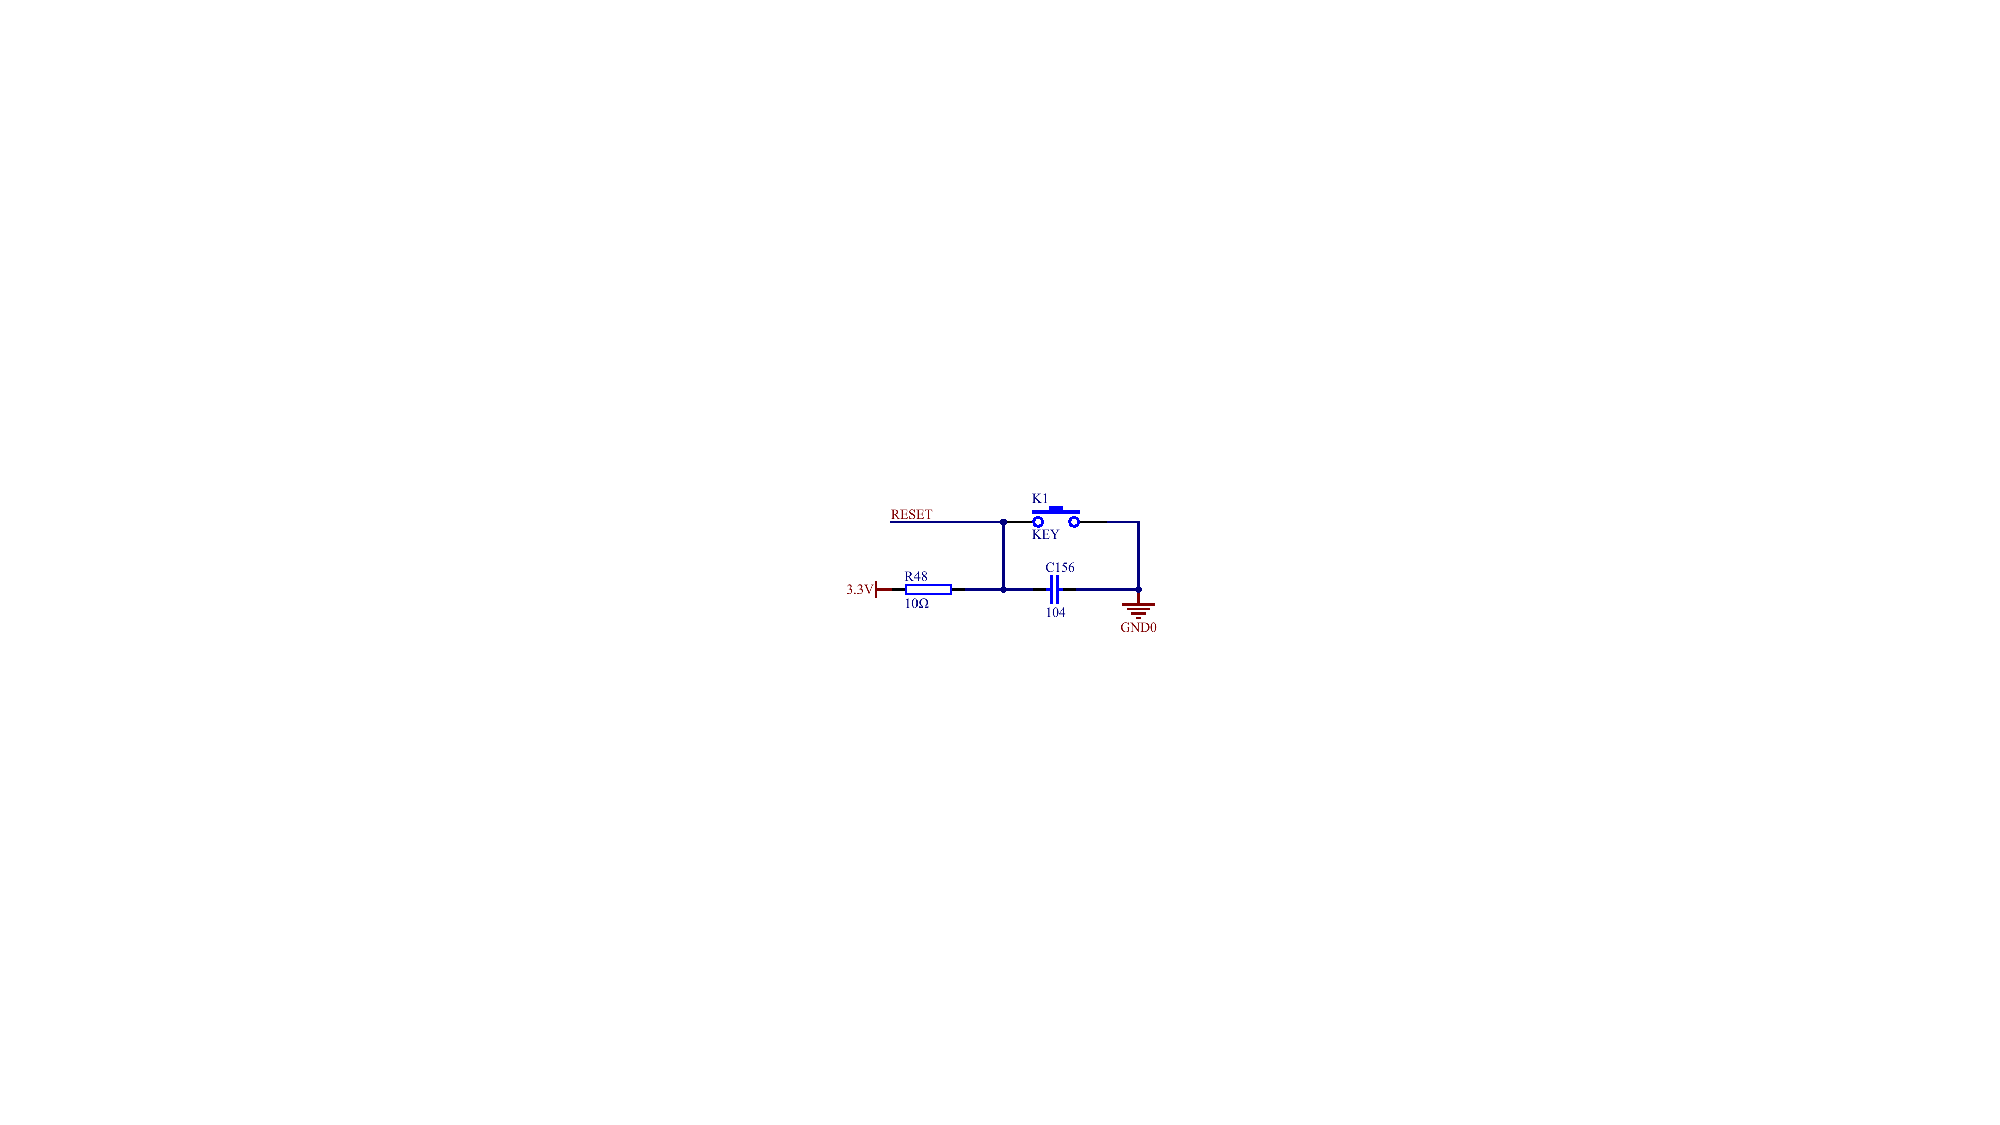
\includegraphics[width=0.24\textheight]{复位电路.pdf}
	\caption{复位电路原理图}
	\label{fig2-9}
\end{figure}

调试电路遵循ARM公司提出的SWD(Serial Wire Debug)协议进行设计。SWD协议能够利用串行通信直接访问ARM Cortex内核的寄存器,在高速模式下比传统的JTAG协议更为可靠。同时,相较于JTAG协议,SWD的引脚数更少,其仅需SWDIO、SWCLK、SWO和RESET四根数据线即可正常工作。这为PCB设计节省了更多的空间,并有效减少了对STM32芯片IO资源的占用。SWDIO:SWD的双向数据信号线,用来提供串行数据的输入输出;SWCLK:SWD的时钟信号线,提供串行时钟输入;SWO:可选择的串行数据输出引脚;RESET:系统复位信号线。本章设计的主控模块通过SWD协议进行程序烧录和Debug调试。

同时,为了能够方便地判断当前设备工作状态,还设计了相关的LED电路。

\subsection{ADS1299采集模块设计}

ADS1299作为采集模块的核心,其将EEG信号的采集、放大、模数转换和数据传输进行了集成。这一设计成功避免了将上述功能分别实现所可能带来的兼容问题以及外界环境干扰,使ADS1299拥有达到110 dB的共模抑制比、低于1 $\mu V_{pp}$的输入噪声和超过500 M$\Omega$的输入阻抗。同时,这一设计也大幅降低了EEG采集系统的开发难度。图\ref{fig2-10}与图\ref{fig2-11}展示了ADS1299的引脚。其具体功能为:

\begin{figure}[h]
	\centering
	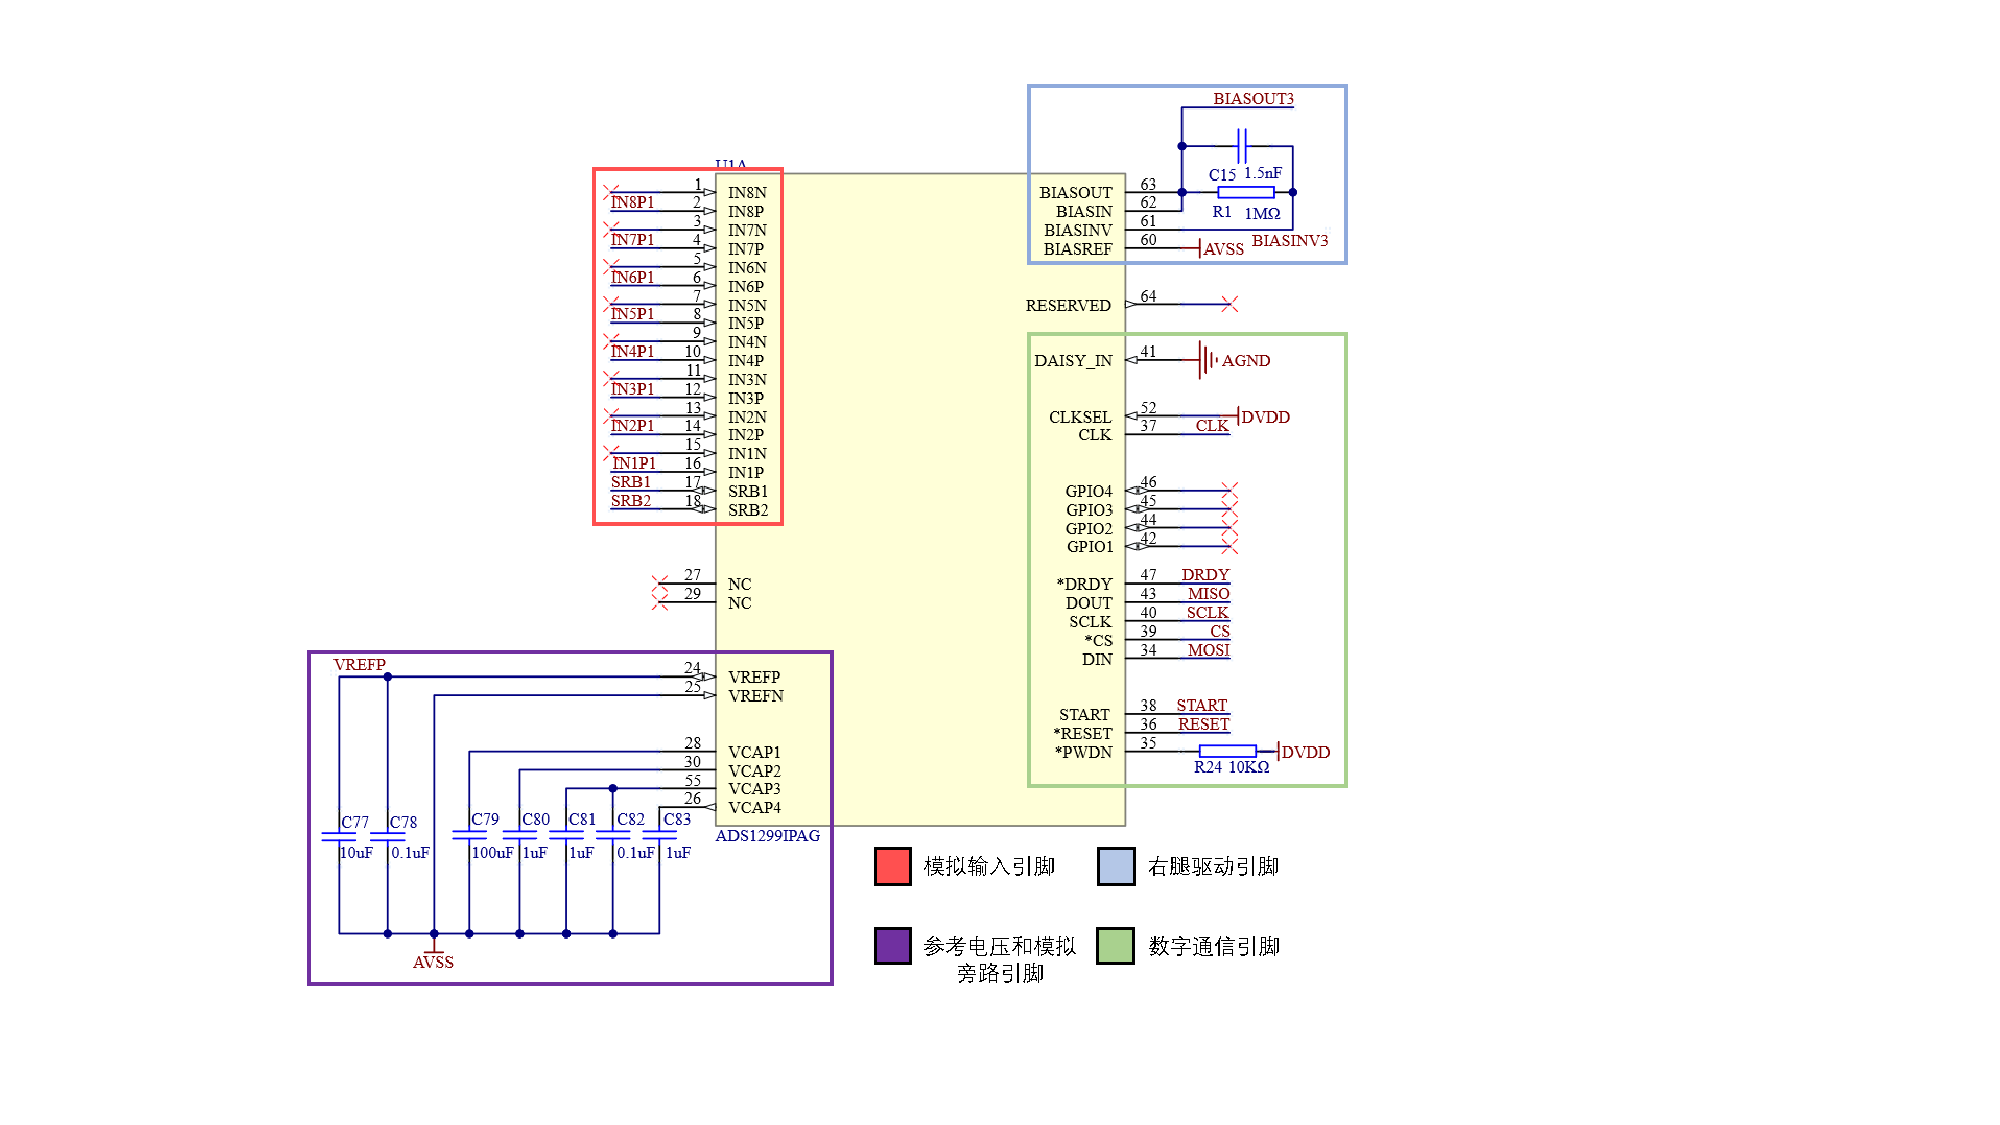
\includegraphics[width=0.605\textheight]{ADS1299功能引脚.pdf}
	\caption{ADS1299功能引脚}
	\label{fig2-10}
\end{figure}


(1) 模拟输入引脚:每块ADS1299芯片具有8通道的模拟差分输入(每个通道包含一个P端和一个N端),即图\ref{fig2-10}中的1-16引脚。同时,还包括了公共端SRB1和SRB2。SRB1/SRB2通过ADS1299内部寄存器进行配置后,可作为所有N/P端的公共引脚。

(2) 参考电压和模拟旁路引脚:参考电压引脚的VREFN端将AVSS接入,用来生成ADS1299内部的4.5 V参考电压。模拟旁路引脚通过电容将电源的高频噪声引向AVSS,防止其干扰采集过程。

(3) 数字通讯引脚:DAISY\_IN引脚用来设置是否采用菊花链式连接;CLKSET用来选择时钟源,高电平时使用内部时钟;CLK引脚用来输出内部时钟信号(内部时钟源)或者接受外来时钟信号(外部时钟源);GPIO是ADS1299正常工作模式下的数字I/O引脚;DRDY是模数转换的标志引脚,拉低时标志转换完成;DOUT,SCLK,CS,DIN是SPI通讯引脚;START引脚和RESET引脚分别控制芯片的启动和复位,其中START高电平生效,RESET低电平生效;PWDN引脚用来控制芯片上电。

(4) 右腿驱动引脚:60-63引脚用来实现芯片的右腿驱动功能,输出反向的共模噪声信号,降低共模干扰。

(5) 电源引脚:如图\ref{fig2-11}所示,遵照ADS1299数据手册要求,完成外围供电电路设计。


\begin{figure}[h]
	\centering
	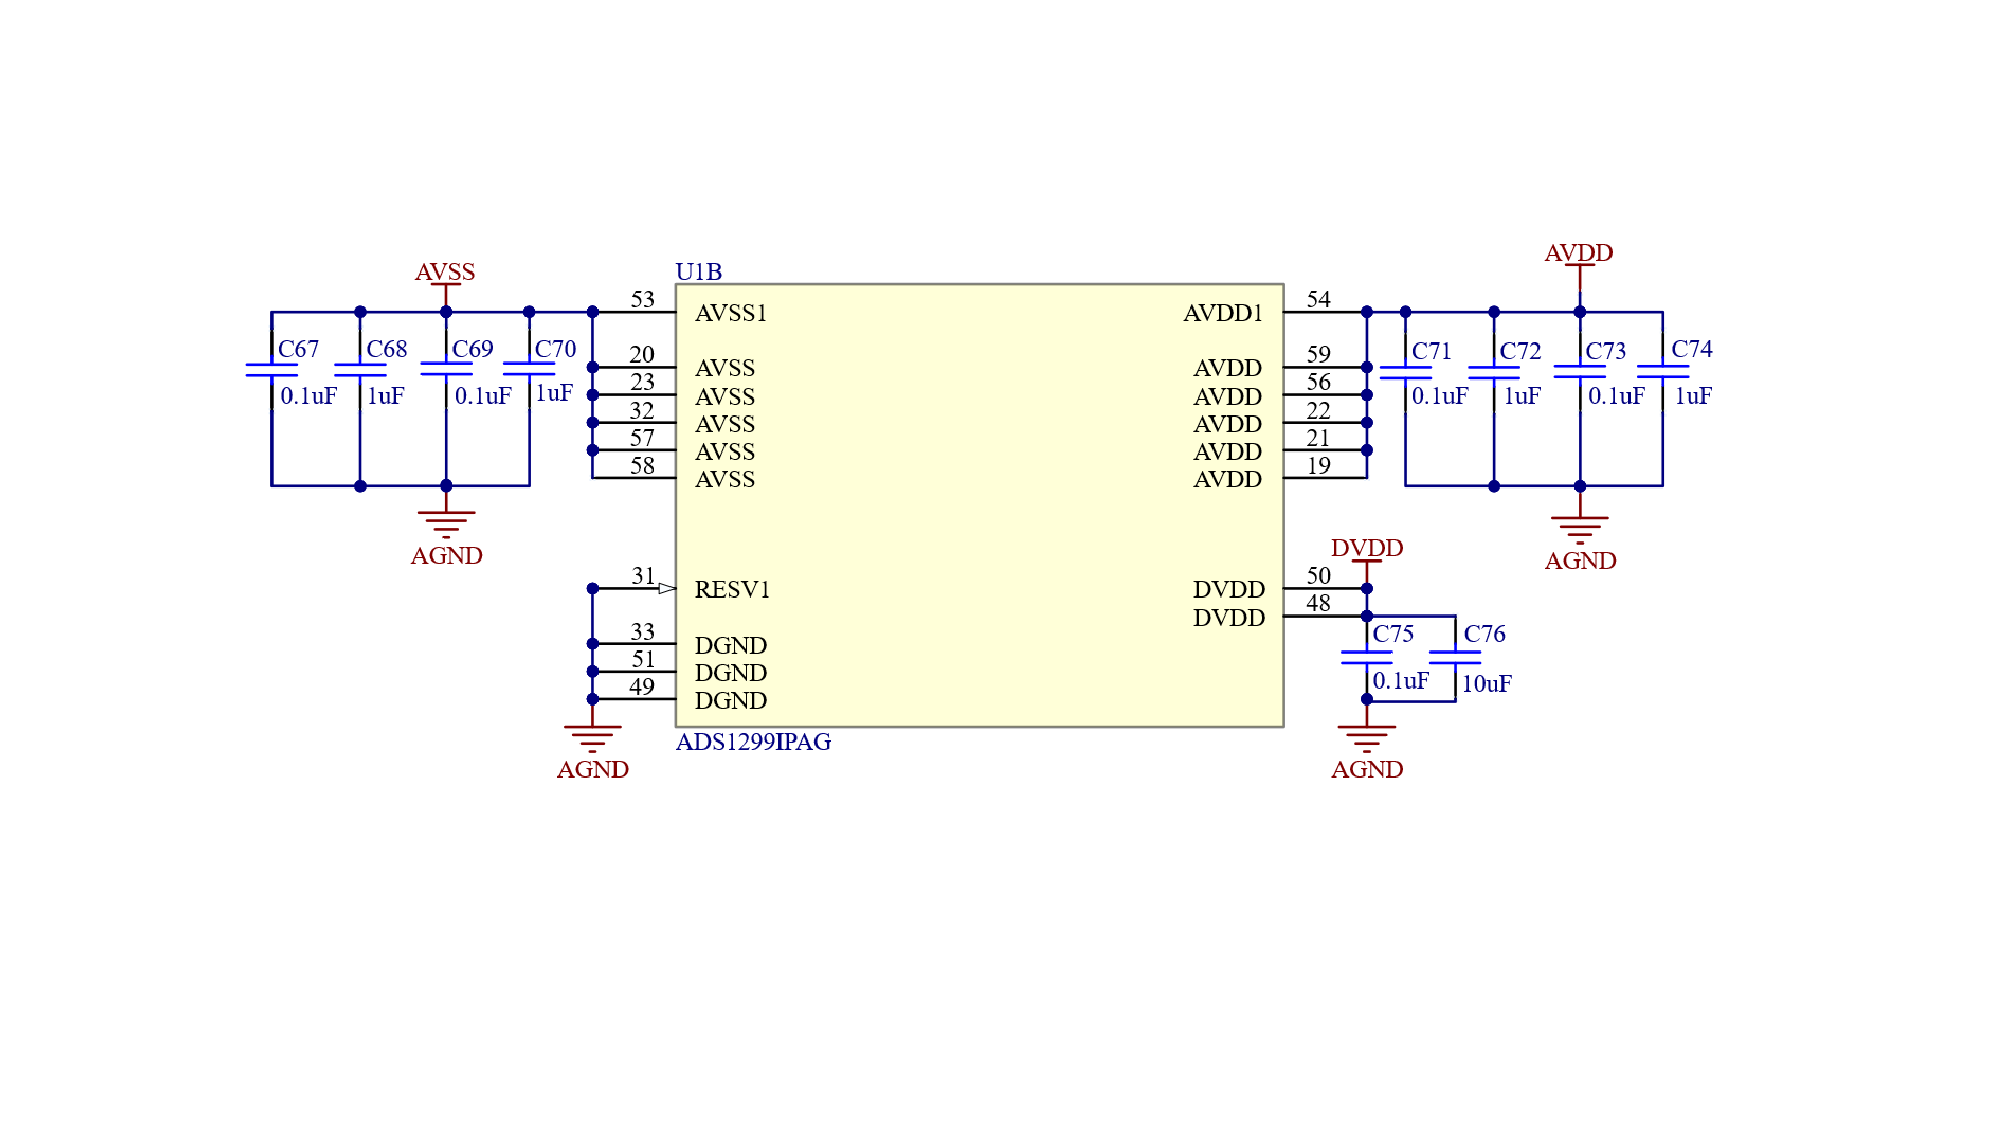
\includegraphics[width=0.61\textheight]{ADS1299电源引脚.pdf}
	\caption{ADS1299电源引脚} 
	\label{fig2-11}
\end{figure}

由于一块ADS1299芯片仅包含8个数据采集通道,因此实现40导联的EEG采集需要5块ADS1299协同工作。ADS1299官方给出了两种不同的多芯片协同方式:标准配置(Standard Configuration)和菊花链配置(Daisy-Chain Configuration)。其中标准配置能够方便地读取所有芯片的寄存器设置,有利于进行设备调试与维护,因此选取标准配置。
\begin{figure}[!h]
	\centering
	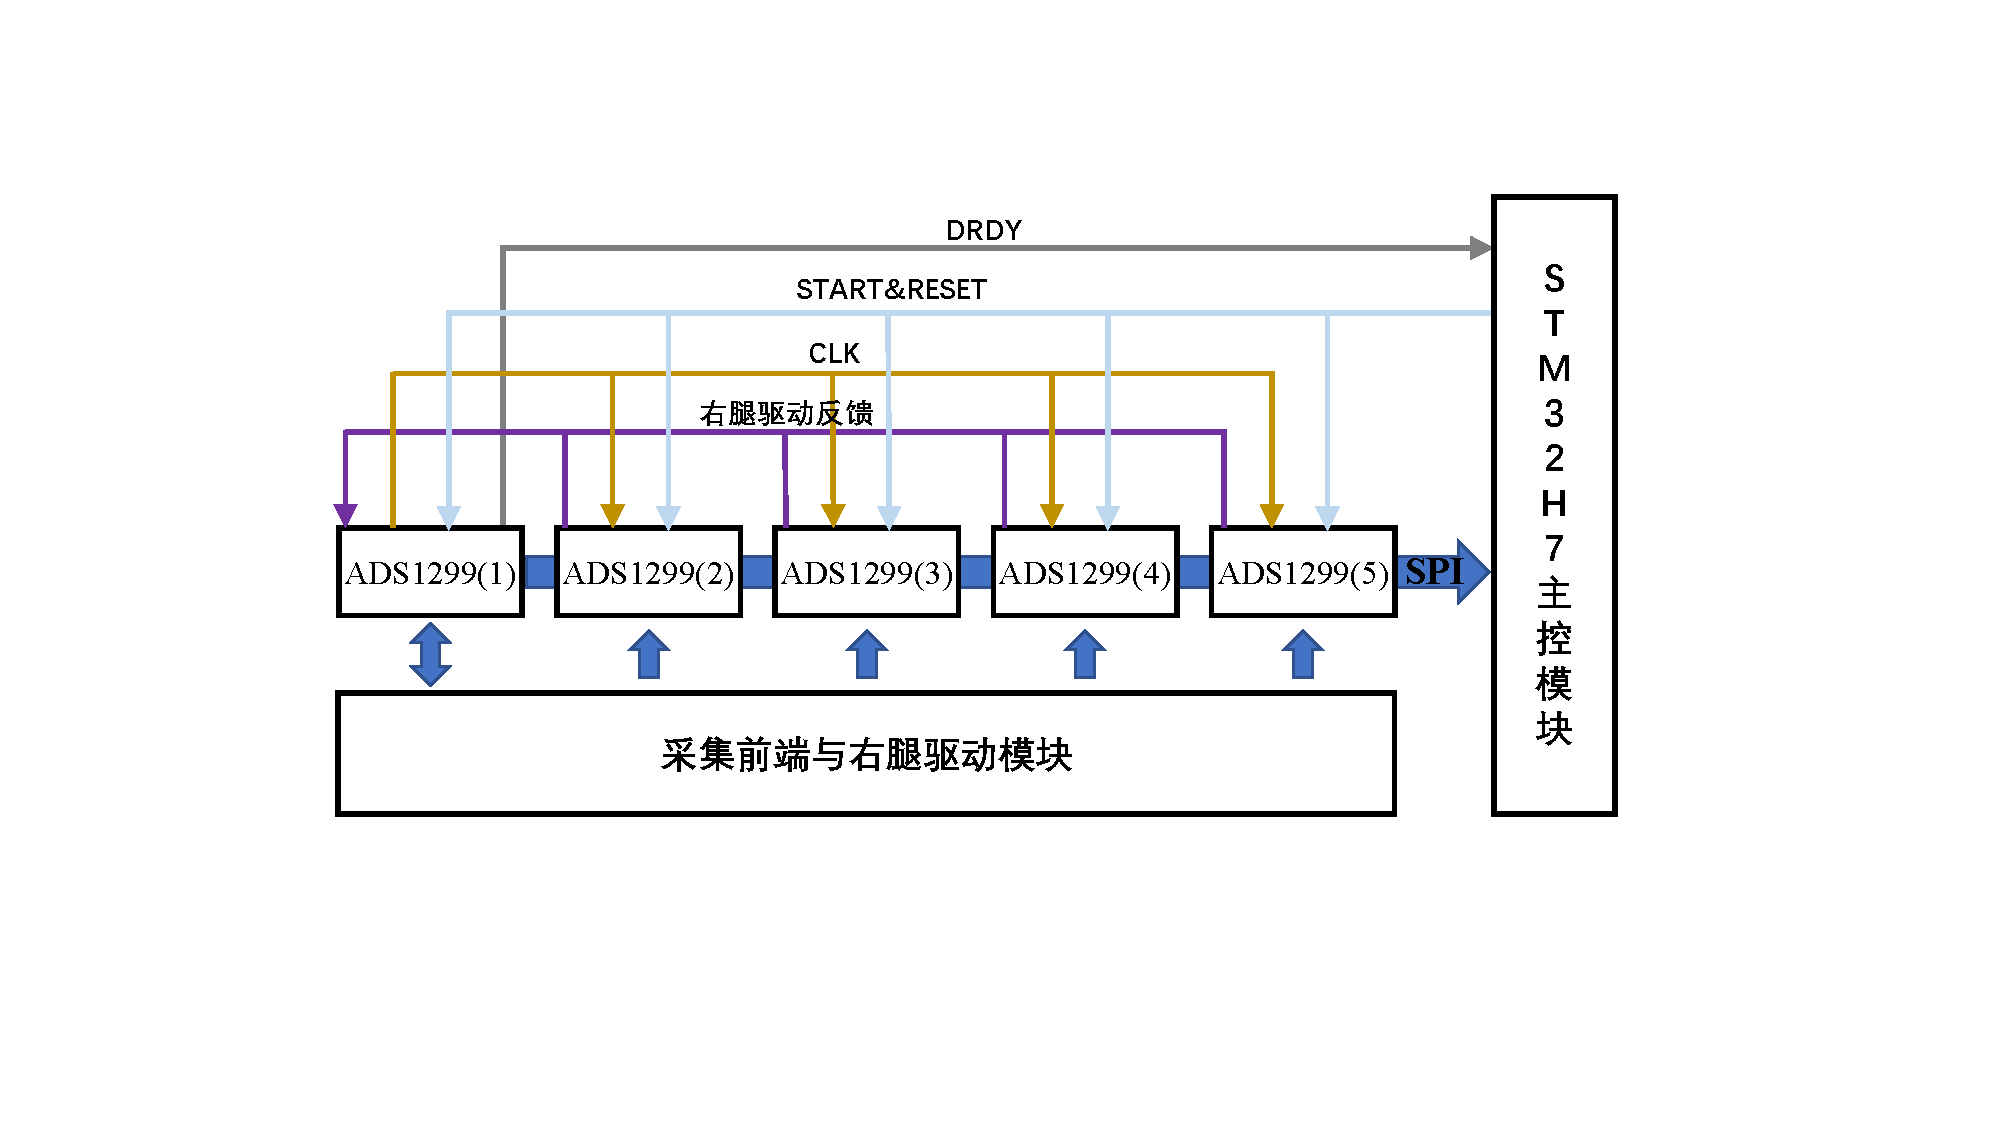
\includegraphics[width=0.5\textheight]{ADS1299连接拓扑图.pdf}
	\caption{ADS1299连接拓扑图} 
	\label{fig2-12}
\end{figure}

本章设计基于标准配置进行,因此首先将DAISY\_IN引脚拉低。接下来,将详细叙述多芯片协同的设计思路。第一步,选取一块ADS1299作为主芯片,开启其内部时钟,并通过寄存器配置其向外输出时钟信号。其他从属芯片使用主芯片的时钟信号,与主芯片保持同步。第二步,在主控模块利用START引脚启动所有芯片后,五块芯片将同时完成数据采集与模数转换,因此只需将主芯片的DRDY接入主控模块即可掌握所有芯片的工作状态。第三步,在DRDY拉低后,通过SPI依次读取所有芯片的数据,实现数据采集。最后,所有从属芯片采集的共模噪声信号将传递给主芯片,统一反馈给人体,消除共模噪声干扰。图\ref{fig2-12}显示了5片ADS1299的连接拓扑图。

\subsection{SPI隔离模块设计}

数字模块和模拟模块之间不仅有电源部分相连,还通过SPI进行数据传输。这可能造成外部噪声进入模拟端,影响EEG数据采集。因此本节在设计时不仅引入了电源隔离模块,还加入了SPI隔离模块。选取川土微公司(Chipanalog)生产的CA-IS3741LN高速四通道数字隔离器作为SPI隔离,其信号传输速率达到150 Mbps、无需启动初始化、传播延迟仅为8 ns并且拥有高达5 $kV_{RMS}$的隔离电压。良好的绝缘能力也使其能够防止其他线路上的噪声和浪涌进入本地接地端,对EEG数据采集造成干扰。经过计算,其参数指标符合当前的设计要求。CA-IS3741LN的原理图如图\ref{fig2-13}。为防止在上电瞬间产生误动,对所有CA-IS3741LN的前向通道增加下拉电阻,保证隔离后信号的确定性。
\begin{figure}[!h]
	\centering
	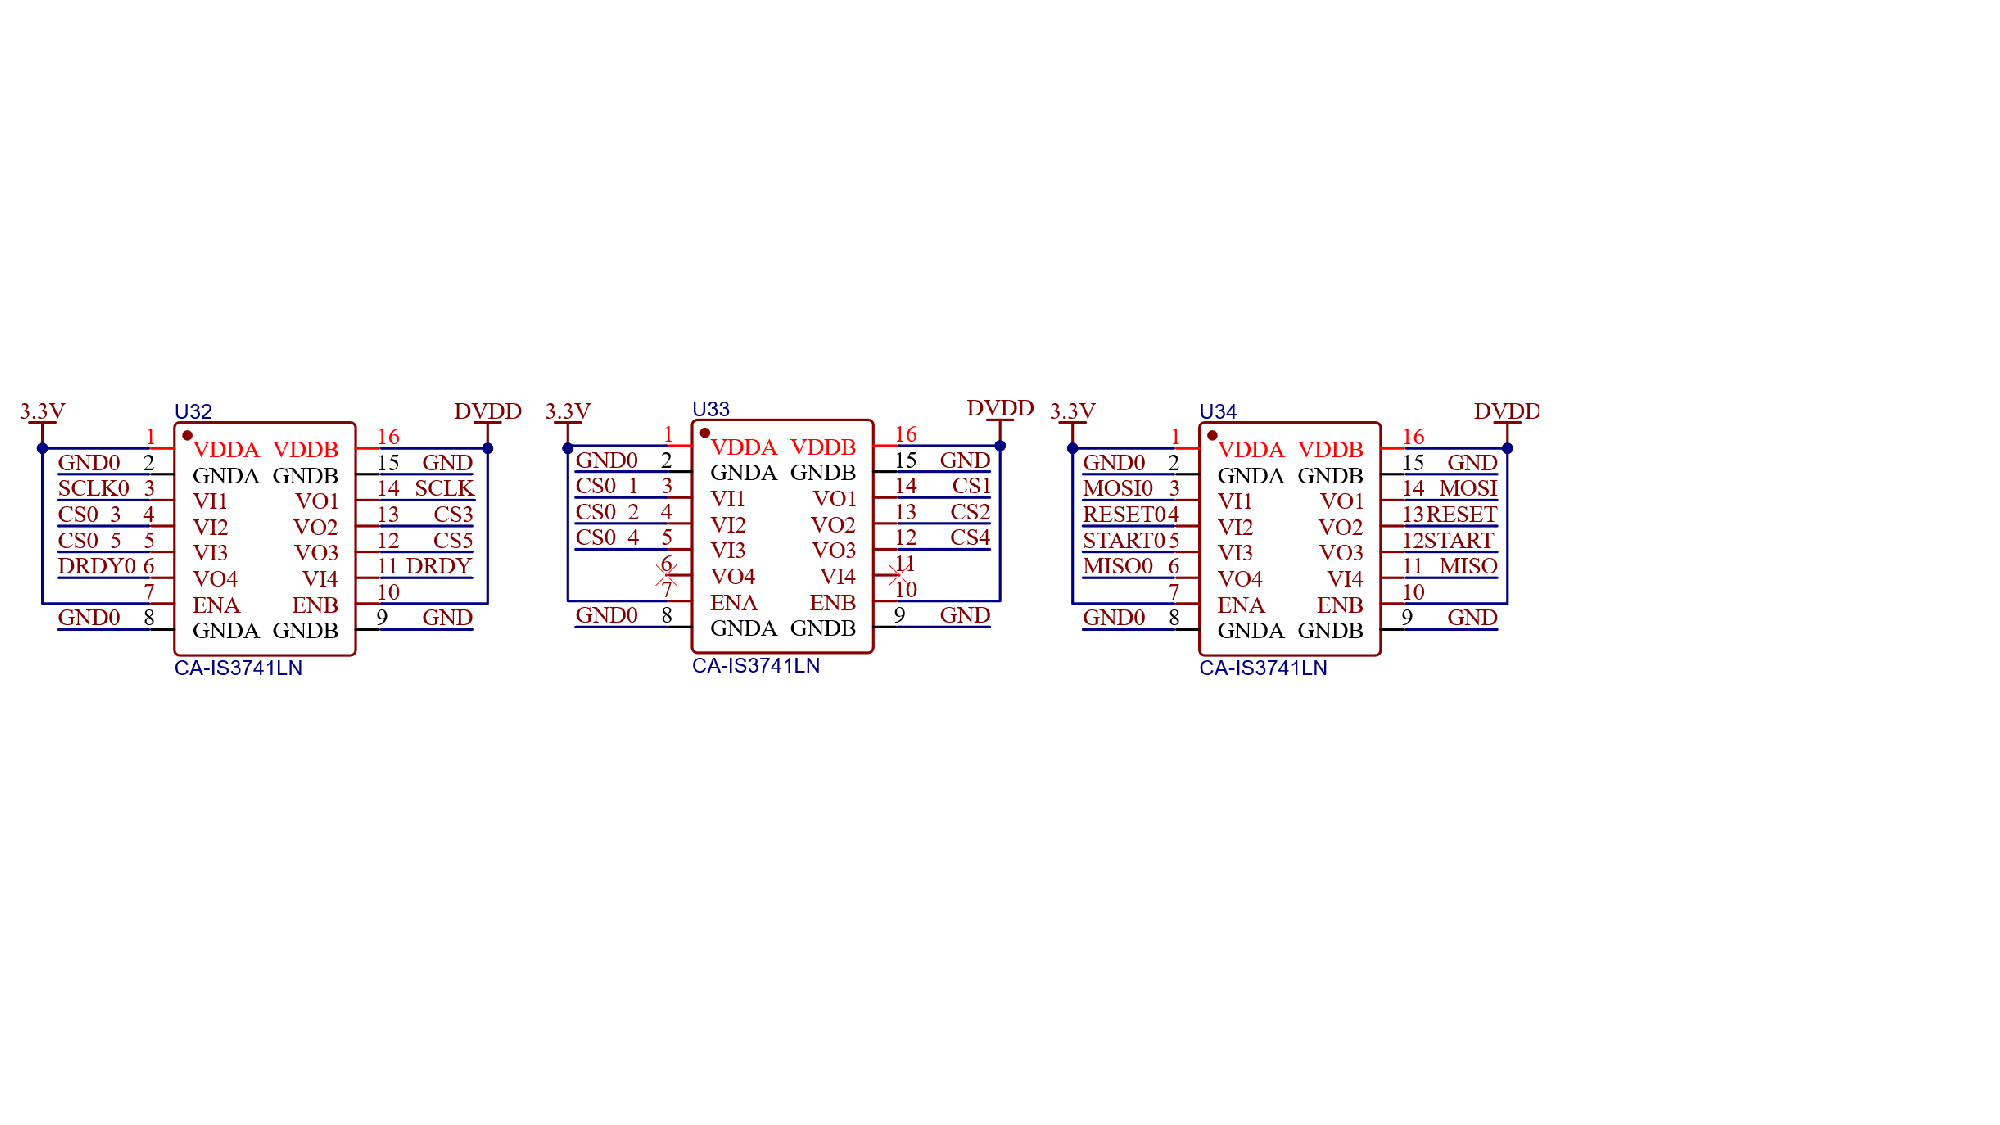
\includegraphics[width=0.61\textheight]{SPI.pdf}
	\caption{SPI隔离模块原理图} 
	\label{fig2-13}
\end{figure}

\subsection{虚拟串口通讯模块}
虚拟串口通讯模块在STM32自带的USB功能上进行实现。STM32H743IIT6内置USB\_OTG\_FS(全速双角色设备控制器)和USB\_OTG\_HS(高速双角色设备控制器),支持作为USB从设备使用的同时还能够作为USB主机使用。USB\_OTG\_FS的理论通讯速度为12 Mbps,符合本章设计需求。同时,相较于USB\_OTG\_HS,其无需外置高速PHY芯片,仅需使用USB\_DM和USB\_DP两个引脚即可实现通信,因此本节采用USB\_OTG\_FS完成设计。

\subsection{采集前端与右腿驱动模块设计}

根据EEG信号的频域特性,在采集前端设计相应的一阶低通滤波电路来对EEG信号进行预处理,消除可能存在的高频噪声。由于EEG信号基本集中在200 Hz以下的频带范围内,因此本节将一阶低通滤波电路的截止频率设计为500 Hz。考虑到RC滤波电路的截止频率计算公式为:

\begin{equation}
    \label{deqn_ex2_2}
    f_c = \frac{1}{2\pi RC}
\end{equation}

考虑到电阻阻值较大时更容易引入噪声,因此选取较小的阻值$\rm R= 800$ $\Omega$,此时$\rm C = 200$ $nF$。这一设计在500 Hz时信号衰减达到$\rm -3$ $dB$,信号功率衰减为原来的50\%。在5 kHz以上时,衰减达到$\rm -20$ $dB$。


人体在采集过程中,无法完全屏蔽周围电磁环境带来的影响。当受到周围电网形成的交流电场作用时,人体表面会产生工频交流电位。作为一种共模干扰,其可能会掩盖生物电信号,对EEG采集造成影响。针对这一问题,右腿驱动电路应运而生。作为一种成功的应对共模干扰的技术,右腿驱动电路被广泛应用于生理电信号测量当中\cite{2-4}。图\ref{fig2-14}展示了右腿驱动电路的具体组成。

\begin{figure}[!h]
	\centering
	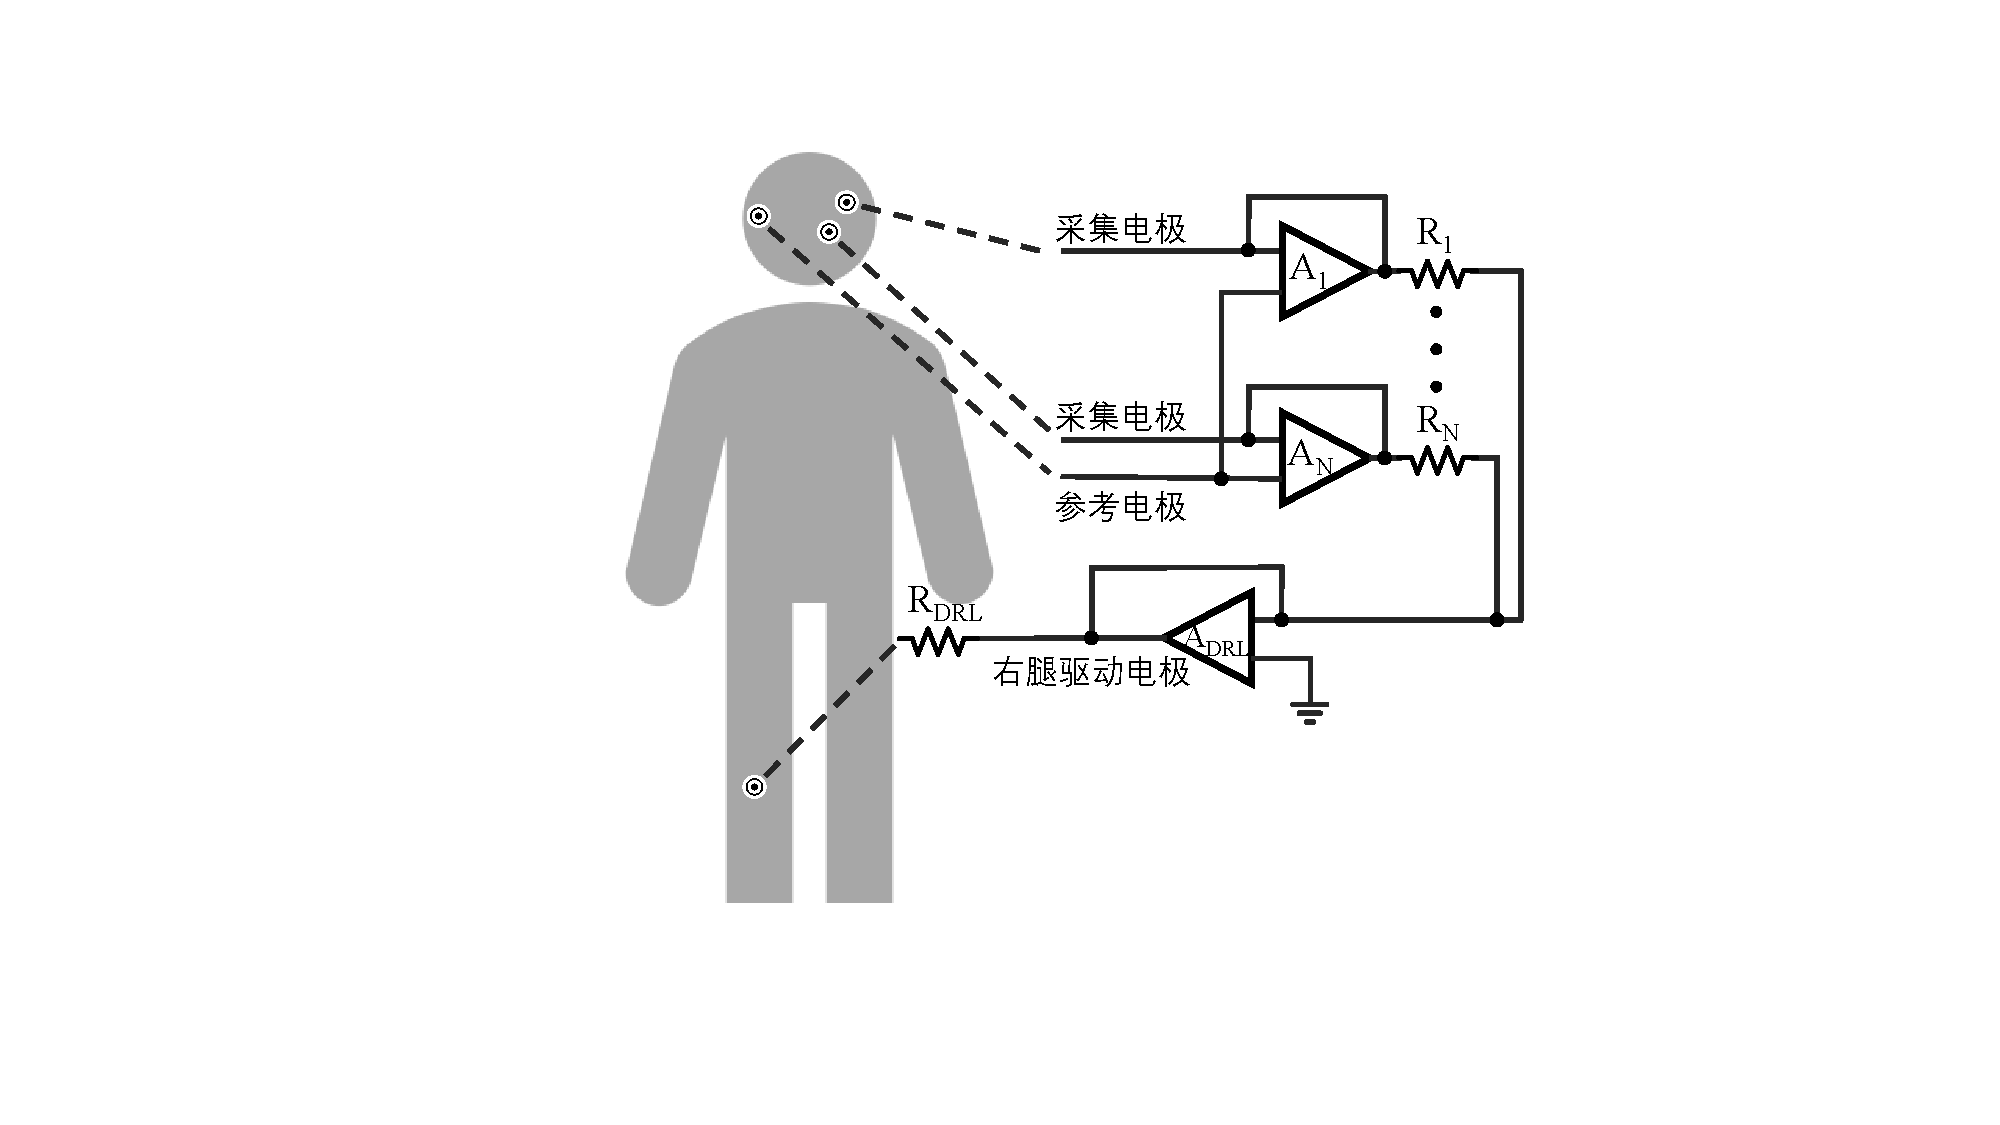
\includegraphics[width=0.35\textheight]{右腿驱动.pdf}
	\caption{右腿驱动电路} 
	\label{fig2-14}
\end{figure}

右腿驱动电路的原理如下所述:首先,EEG电极采集得到的原始EEG信号,经由一组低噪声PGA $\rm A_1-A_N$组成的差分放大电路传递至$\rm R_1-R_N$,此时的原始信号中包含了大量的共模分量。接下来,通过$\rm R_1-R_N$的共模信号在累加后被$\rm A_{DRL}$反向放大,经由$\rm R_{DRL}$重新传递回受试者皮肤表面以消除共模干扰。本节在设计时,综合考量受试者的使用习惯并参考ADS1299的数据手册,将参考电极放置在左耳后乳突处,将右腿驱动电极放置在右耳后乳突处。

\begin{figure}[h!]
	\centering
	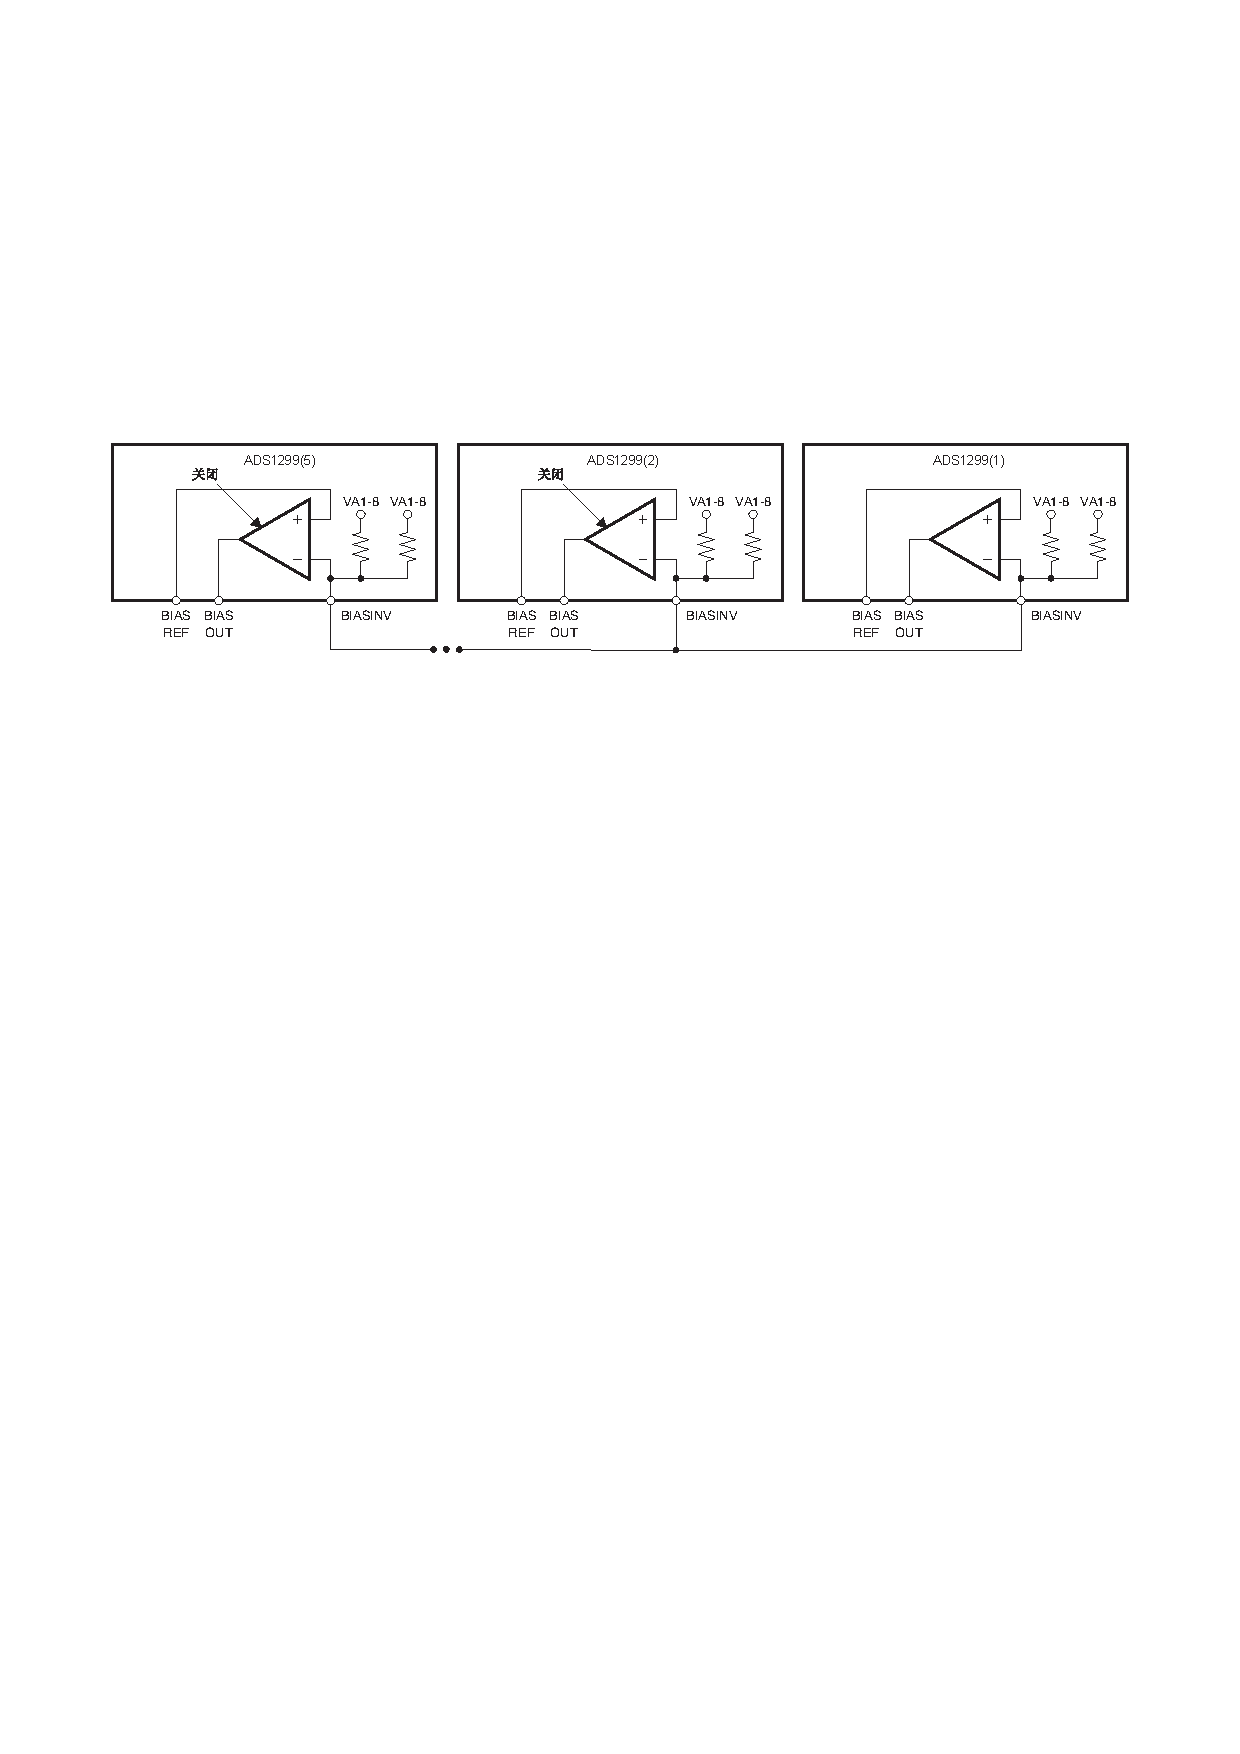
\includegraphics[width=0.605\textheight]{右腿驱动级联.pdf}
	\caption{ADS1299多芯片右腿驱动配置} 
	\label{fig2-15}
\end{figure}

ADS1299中已经集成了右腿驱动电路,本节在设计时只需考量如何对多组电路进行协同。多芯片级联方式如图\ref{fig2-15},开启主ADS1299芯片的$\rm A_{DRL}$,关闭其他从芯片的$\rm A_{DRL}$,将所有的共模信号累加至主芯片后统一反馈给人体。

\subsection{静电与过载保护设计}
考虑到EEG采集的实际使用环境,为了防止静电从与外界接触的采集端,USB输入端以及开关按钮处进入PCB内部,干扰数据采集甚至影响设备运行,本节在相应位置引入了静电放电(Electro-Static Discharge,ESD)保护芯片。在充分考虑设备的电磁兼容性问题后,三款不同的ESD保护芯片被分别设计在PCB的采集端,USB输入端以及开关按钮的电路中。详细设计如下:

\begin{figure}[!h]
	\centering
	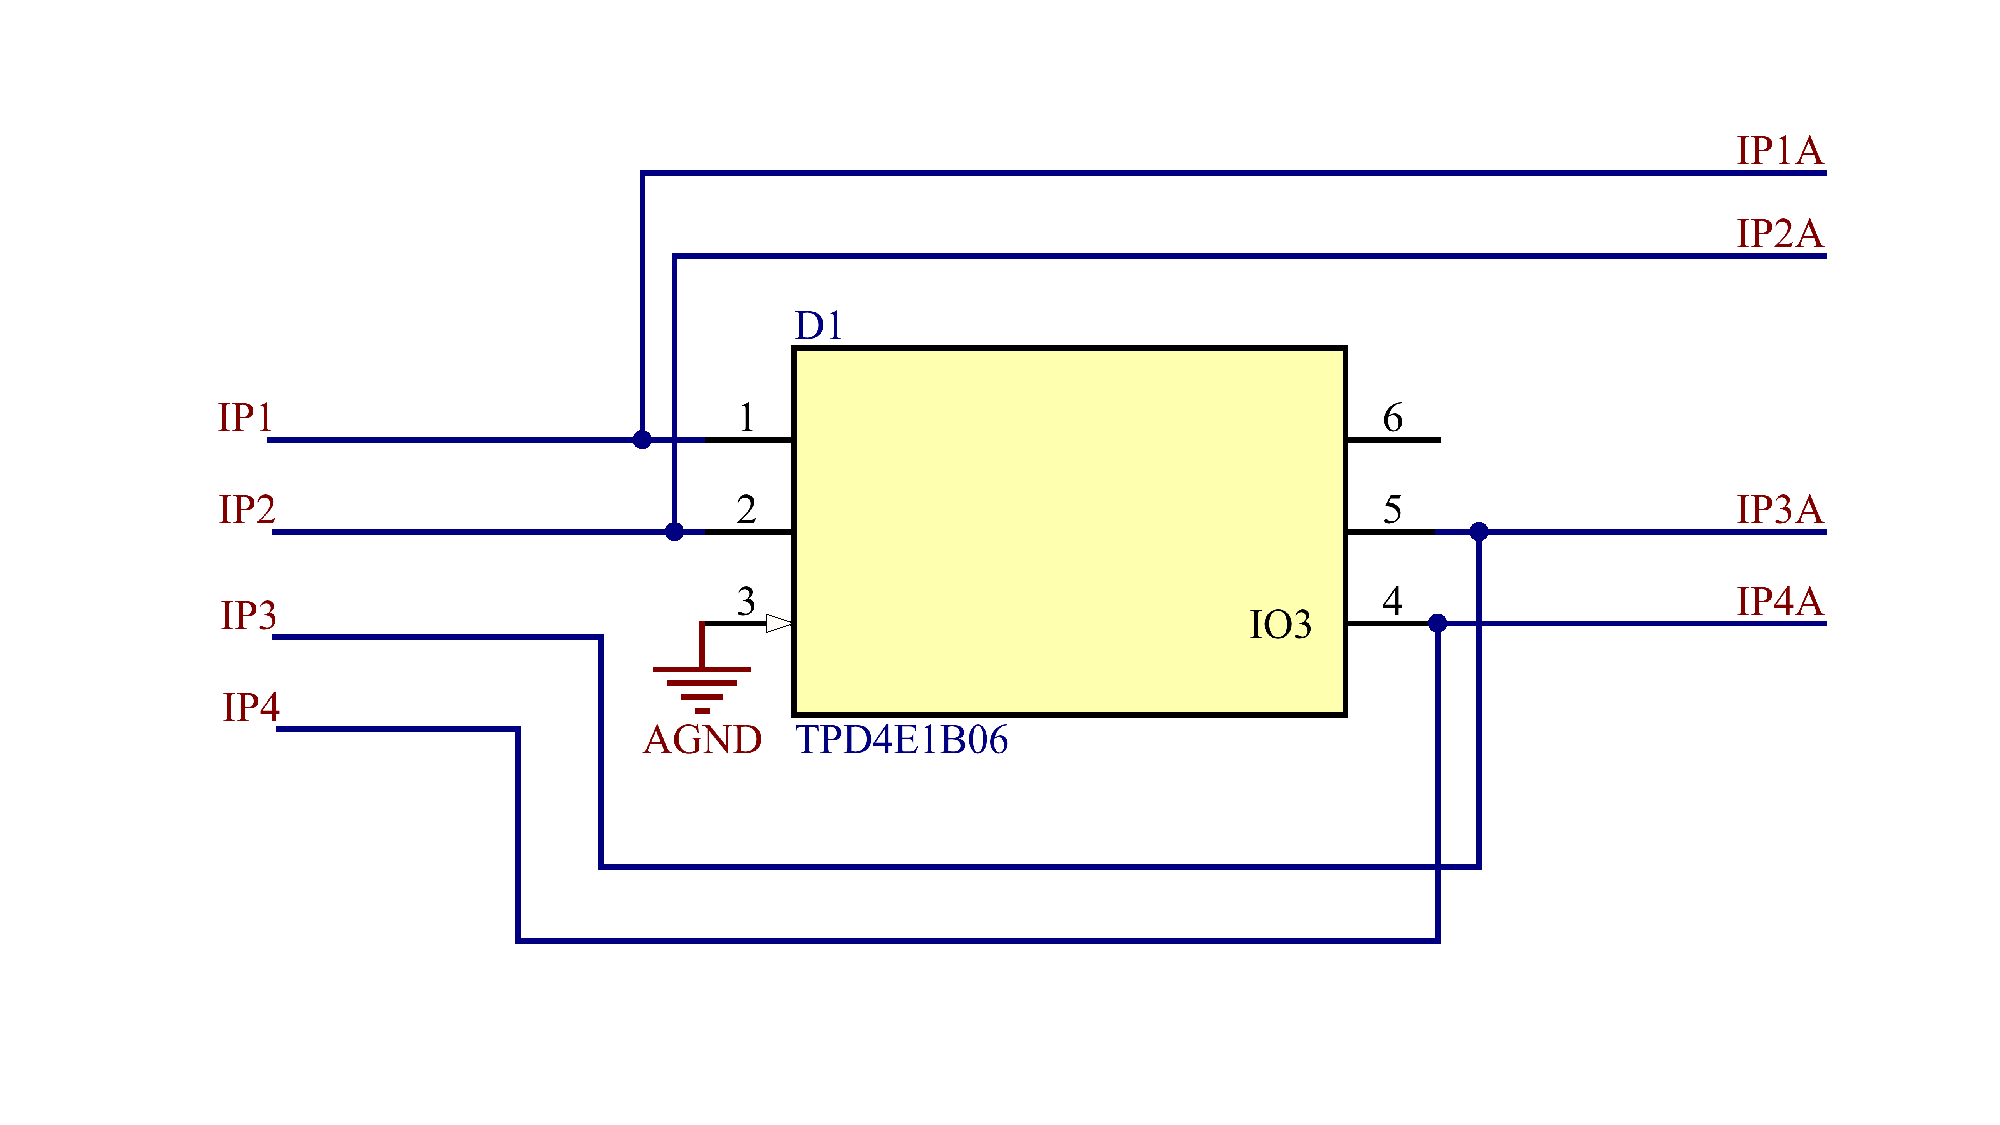
\includegraphics[width=0.42\textheight]{采集端ESD.pdf}
	\caption{TPD4E1B06原理图} 
	\label{fig2-16}
\end{figure}

(1) 采集前端处,使用TPD4E1B06 4通道ESD保护器件保护采集端口。TPD4E1B06是德州仪器公司设计的一款4通道双向瞬态电压抑制器(Transient Voltage Suppressor,TVS)二极管阵列。这款芯片能够为设备提供$\pm12$ kV的接触和$\pm15$ kV空气间隙放电保护。其漏电流仅为0.5 nA,能够为模拟信号的精确测量提供保障。$\rm 0.7$ pF的线路电容值使其能够应用于医疗设备之中。同时,如图\ref{fig2-16}所示,TPD4E1B06的电路无需引入额外器件,大幅简化了ESD电路设计。

\begin{figure}[h]
	\centering
	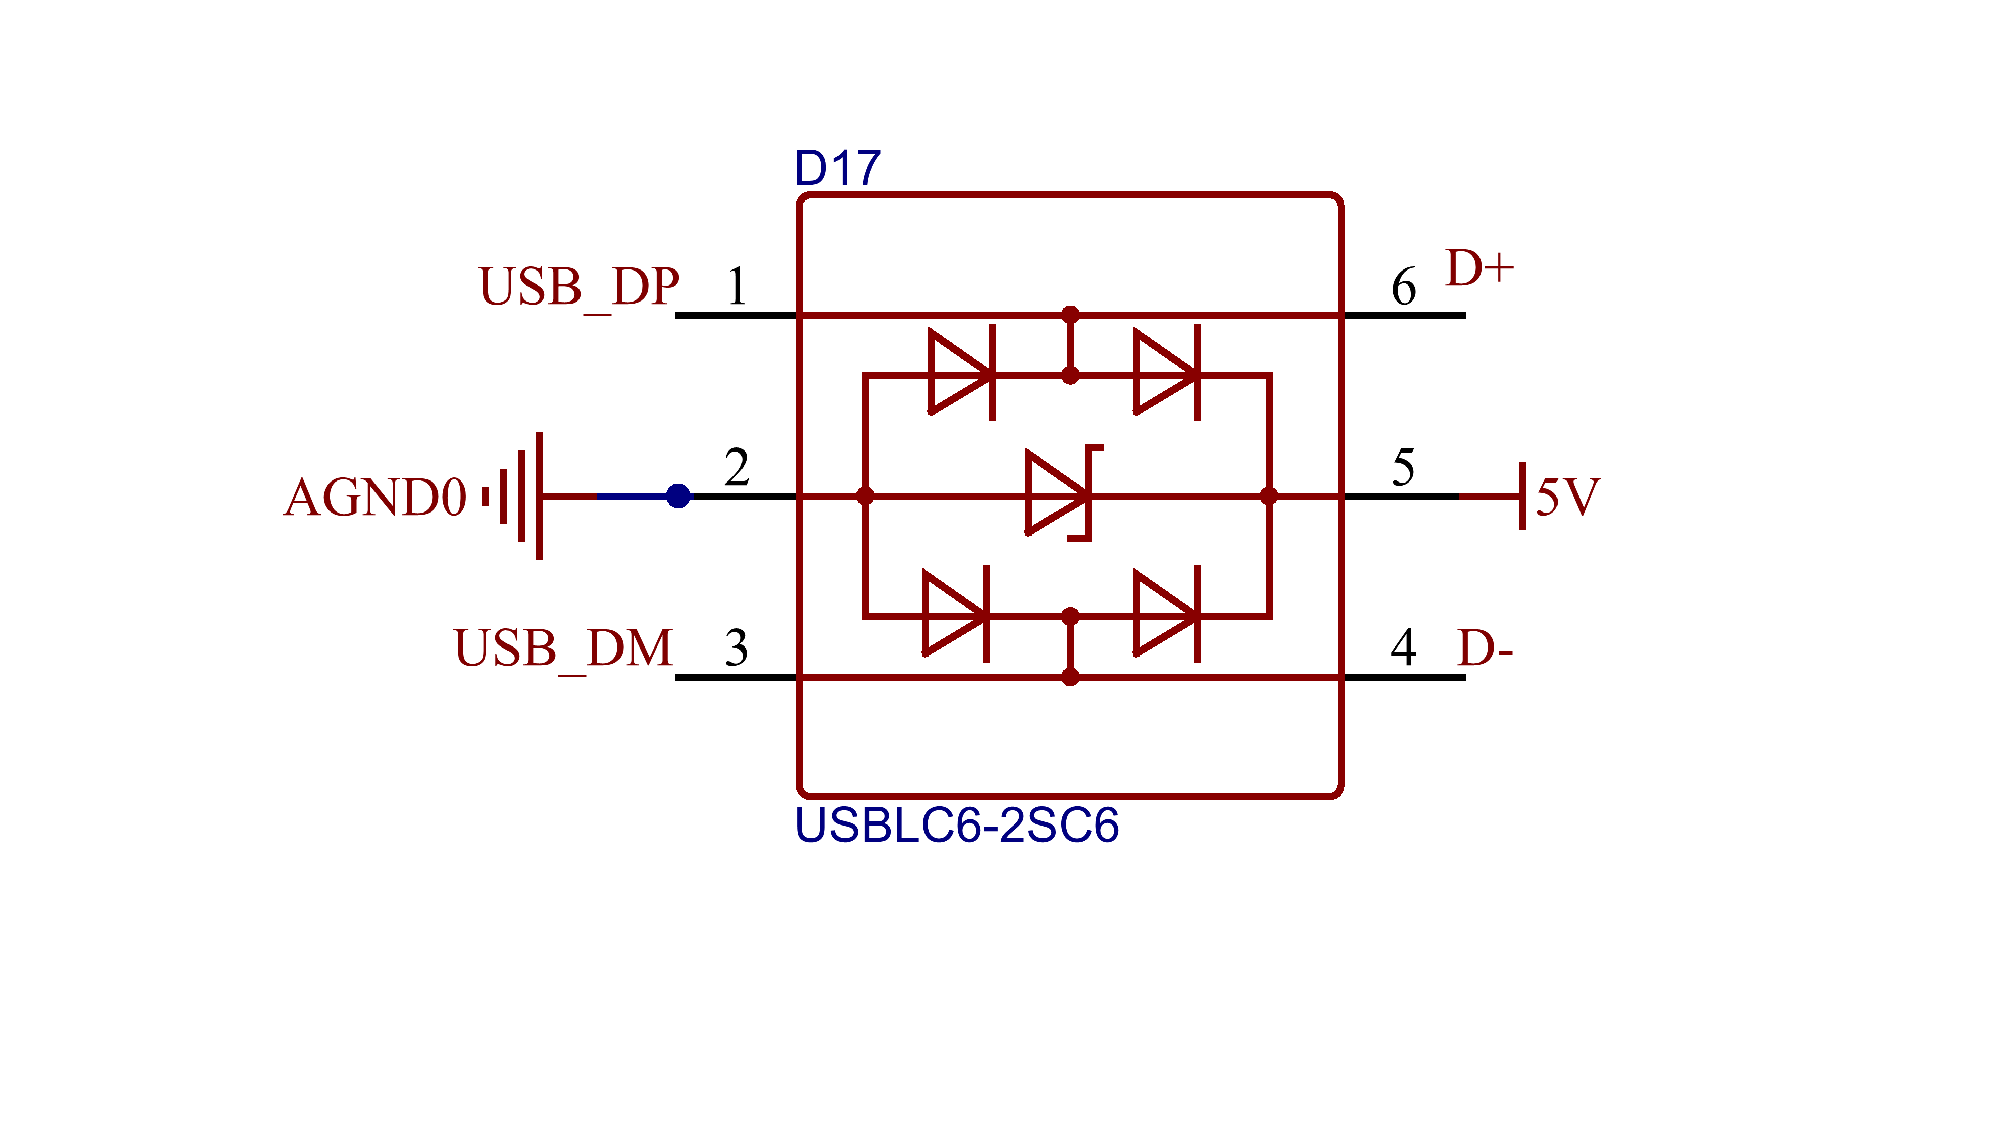
\includegraphics[width=0.28\textheight]{USB_ESD.pdf}
	\caption{USBLC6-2SC6原理图} 
	\label{fig2-17}
\end{figure}


(2) USB输入端引入USBLC6-2SC6进行ESD保护。USBLC6-2SC6是意法半导体公司为USB通讯电路设计的专用ESD保护芯片,其能够同时保护两条USB通信线路,I/O与地之间的电容匹配公差仅为0.015 pF,典型电容值不超过3.5 pF,符合USB 2.0的通讯需求。USBLC6-2SC6能够为设备提供$\pm8$ kV的接触和$\pm15$ kV空气间隙放电保护。其原理图如图\ref{fig2-17}所示。

(3) 为了避免静电经由开关进入PCB,在开关处引入PSOT05C-LF-T7芯片。PSOT05C-LF-T7为PROTEK公司设计的TVS二极管阵列,被广泛应用于电源线路保护。其能够在3 V-36 V的电压下工作,为系统提供$\pm8$ kV的接触和$\pm15$ kV空气间隙放电保护。同时其能够承受500 W的峰值脉冲功率(上升沿8 us,半峰值20 us下),符合设计要求。其原理图如图\ref{fig2-18}所示。

\begin{figure}[h]
	\centering
	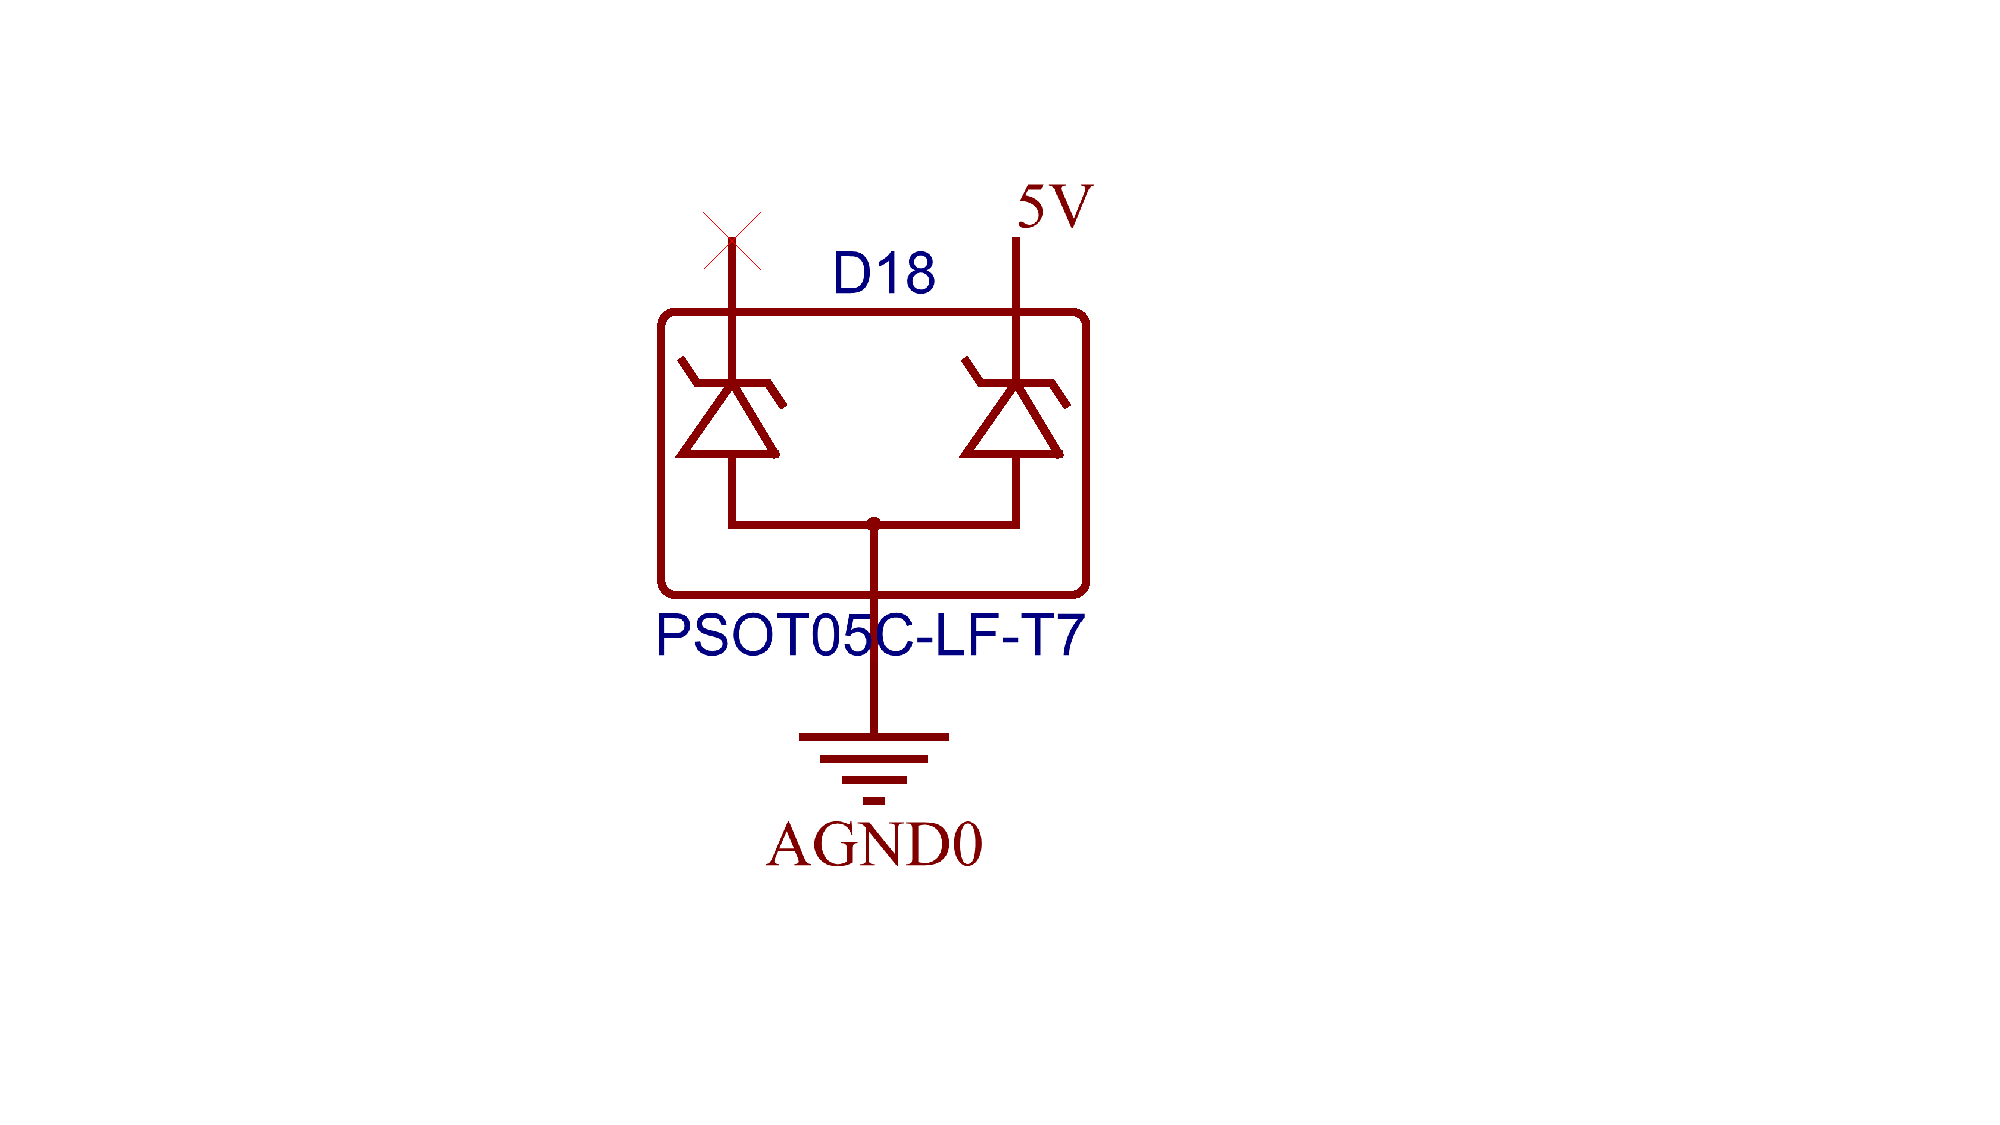
\includegraphics[width=0.08\textheight]{开关ESD.pdf}
	\caption{PSOT05C-LF-T7原理图} 
	\label{fig2-18}
\end{figure}

为保证设备能够在过载情况下进行自我保护,防止芯片损坏,在USB端口的供电处设计了自恢复保险丝。保险丝型号的选取考虑以下两点:(1) 采集模块的工作电流。测量得到采集模块正常工作时的电流为285 mA,与计算值基本相符。(2) USB端口供电能力。USB 2.0端口的供电能力为5 V/500 mA。综上所述,选取ASMD1210-050作为保险丝,其熔断电流为500 mA,符合设计需求。



\section{JS-AINS-40系统软件设计}
在硬件内容的基础上,本节介绍JS-AINS-40系统配套的软件设计。软件设计主要包括采集模块的下位机软件和上位机的软件两部分,其中下位机软件运行在STM32H743IIT6的嵌入式平台,上位机软件运行在Windows PC端。
\subsection{下位机软件设计}
利用C语言编写的下位机软件主要实现的功能包括:通过STM32H743IIT6主控模块经由SPI隔离模块控制ADS1299采集模块,使其按照性能要求采集EEG数据。接收ADS1299采集模块回传的数据,裁剪拼接后通过虚拟串口通讯模传递给上位机。

(1) STM32H743IIT6主控模块主程序

\begin{figure}[h]
	\centering
	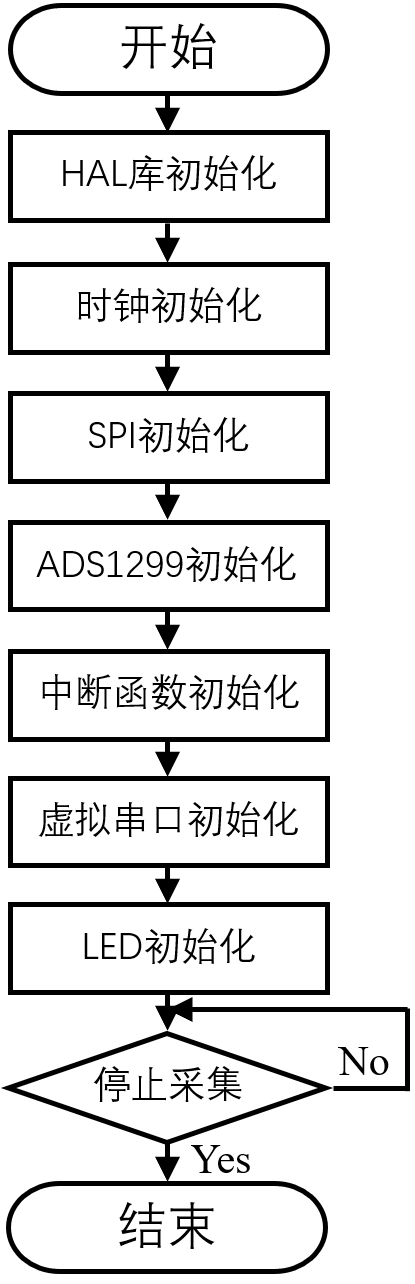
\includegraphics[width=0.13\textheight]{下位机主程序.png}
	\caption{STM32H743IIT6主控模块主程序流程图} 
	\label{fig2-19}
\end{figure}

STM32H743IIT6主控模块主程序主要负责进行初始化。其首先初始化STM32H743IIT6芯片的HAL库和时钟,保证主控芯片开始正常运行。之后初始化SPI模块,保证主控芯片能够通过SPI初始化ADS1299。ADS1299初始化时,STM32H743IIT6主控芯片将根据具体的使用需求配置ADS1299的内部寄存器,保证其正常采集。中断函数和虚拟串口初始化后将保证主控芯片能够识别ADS1299发来的数据转换完成信号,并将接收到的数据发送给上位机。最后,LED初始化后将作为设备工作状态的指示灯。具体流程如图\ref{fig2-19}所示。

在所有设备初始化结束后,主控芯片将自动读取每一片ADS1299的控制寄存器,确认其是否与初始化时设置的一致。如果存在差异,则LED指示灯将通过不同次数的闪烁告知使用者出现问题的ADS1299编号,并通过虚拟串口向上位机发送提示使用者进行设备重启的字符。如果不存在差异,则认为设备正常启动,向上位机发送已准备就绪的字符,并进入准备状态,等待运行指令。


(2) ADS1299 控制程序

主控芯片通过SPI初始化ADS1299的流程为:

1) 拉低RESET引脚,对ADS1299进行复位,并在20 ms后拉高RESET引脚。在间隔20 ms后再次拉低RESET引脚,并在20 ms后拉高RESET引脚。重复执行这一过程,是为了保证ADS1299复位成功。(这期间,START引脚始终保持低电平)

2) 向第一片ADS1299芯片发送停止连续读取指令,并停顿20 ms,保证指令生效。

3) 向第一片芯片发送控制寄存器1的配置指令。寄存器1负责控制多芯片的级联方式,是否向外输出内部时钟以及EEG数据的采样率。根据硬件设计章节的叙述,这里选择使用标准配置来级联多块ADS1299,因此寄存器1设置为多重回读模式(Multiple Readback Mode)。同时,由于第一块ADS1299芯片作为主芯片需要给从属芯片提供时钟,因此这里设置向外输出内部时钟。最后,EEG信号的采样率根据任务要求具体设置。注意,这一步骤结束后需要等待50 ms,以保证主芯片的时钟趋于稳定,这时才能够成功初始化从属芯片。

4) 向所有从属ADS1299芯片发送停止连续读取指令,并停顿20 ms,保证指令生效。

5) 向所有从属ADS1299芯片发送控制寄存器1的配置指令。从属芯片接收外来时钟,因此配置与主芯片略有不同。

6) 向第一片芯片发送控制寄存器3的配置指令。控制寄存器3负责右腿驱动模块的设置,基于硬件设计章节的叙述,开启主ADS1299芯片的右腿驱动电路。

7) 向所有从属ADS1299芯片发送控制寄存器3的配置指令,关闭其右腿驱动电路。

8) 对剩余所有控制寄存器配置,主从ADS1299芯片均保持一致。按照要求依次在对应控制寄存器中配置工作模式(正常电极输入)、差分输入模式(共差分输入,SRB1作为公共端)、参考类型(使用内部参考)、PGA增益(本章设计时选取24)。

9) 发送连续转换指令,进入准备状态。

经过上述流程,ADS1299被成功初始化。在STM32H743IIT6芯片接收到上位机发送的运行指令后,将把ADS1299的START引脚拉高,使其开始信号采集与模数转化。当一次模数转化完成后,ADS1299的DRDY引脚被拉低,进而触发在STM32H743IIT6芯片的中断程序。

(3) 中断程序

STM32H743IIT6主控芯片将主ADS1299芯片的DRDY引脚设置为外部中断源。当进入中断程序时,主控芯片会依次读取五块ADS1299的全部数据。每片ADS1299的数据有216 bits,其中前24位为芯片状态位(1100 + LOFF\_STATP + LOFF\_STATN + GPIO寄存器的4-7位),后192位为8个通道的EEG数据。每个通道的数据由24位补码表示,根据数据手册,其中一位的分辨率(Least Sigificant Bit,LSB)为:

\begin{equation}
    \label{deqn_ex2_3}
    1\ \mathrm{LSB}=\left(2 \times \mathrm{V}_{\mathrm{REF}} / \text { Gain }\right) / 2^{24}=+\mathrm{FS} / 2^{23}
\end{equation}

其中$\mathrm{V}_{\mathrm{REF}}$为参考电压(本章设计中为4.5 V),$\text{Gain}$为PGA增益(本章设计时选取24),$-\mathrm{FS}$至$+\mathrm{FS}$为ADS1299的采集范围。不同的信号幅度与对应输出结果间的关系如表\ref{tab2-1}:

\begin{table*}[!h]
\caption{输入信号幅度与转换结果对应关系}  \label{tab2-1}
\centering
\wuhao{
    \begin{threeparttable}
    \setlength{\tabcolsep}{5mm}{
        \begin{tabular}{cc}
            \toprule
            信号幅度 &转换结果\\
            \midrule
            $\geq F S$                                 &7FFFFFh \\
            $+F S /\left(2^{23}-1\right)$              &000001h \\
            0                                          &0 \\
            $-F S /\left(2^{23}-1\right)$              &FFFFFFh  \\
            $\leq-F S\left(2^{23} / 2^{23}-1\right)$   &800000h\\
            \bottomrule
        \end{tabular}
        }
    \end{threeparttable}
    }
\end{table*}

本设计并不关心芯片状态位,因此直接舍去前24位,仅保留每个芯片的后192位数据进行拼接,并通过虚拟串口发送函数发送给上位机。考虑到下位机的计算资源有限,输入信号的幅度转换放置在上位机中进行。

(4) 虚拟串口通讯程序

STM32CubeMX软件由意法半导体公司开发,作为STM32芯片配套的辅助开发工具。其能够通过图形化的界面快速生成相应的程序代码,大幅简化开发流程。因此在本节,使用STM32CubeMX软件生成相应的虚拟串口通讯程序。具体设置流程为:首先,选择STM32H743IIT6芯片;之后在外设界面选择添加USB,并选取FS通道;接下来添加中间件,选择CDC虚拟串口;最后,设置时钟并生成工程代码。利用生成的工程模板中的虚拟串口发送函数,即可实现向上位机的数据发送。由于虚拟串口每次发送需要消耗一定的时间,这在ADS1299处于高采样率时可能导致数据丢包。因此,主控芯片会将每个DRDY中断后得到的EEG数据暂时进行存储,在中断次数达到8次后统一进行发送,即传输960(8 × 5 × 24)字节的数据。为了保证数据传输的完整性,在960字节数据末尾添加CRC校验位——由下位机计算CRC校验值后,一次向上位机发送961字节数据。

\subsection{上位机软件设计}

上位机程序能够向使用者反馈下位机的当前状态,引导使用者进行设备重启或者开始采集、能够操控采集设备的启动与停止、能够接收下位机传送的EEG数据并进行幅度转换、能够根据转换后的EEG数据实时绘制波形图、能够在接收EEG数据时同步保存转换后的EEG数据,并且能够配合EEG实验引导界面为EEG数据进行标签标注。软件界面如图\ref{fig2-20}所示。具体使用流程为:

\begin{figure}[h]
	\centering
	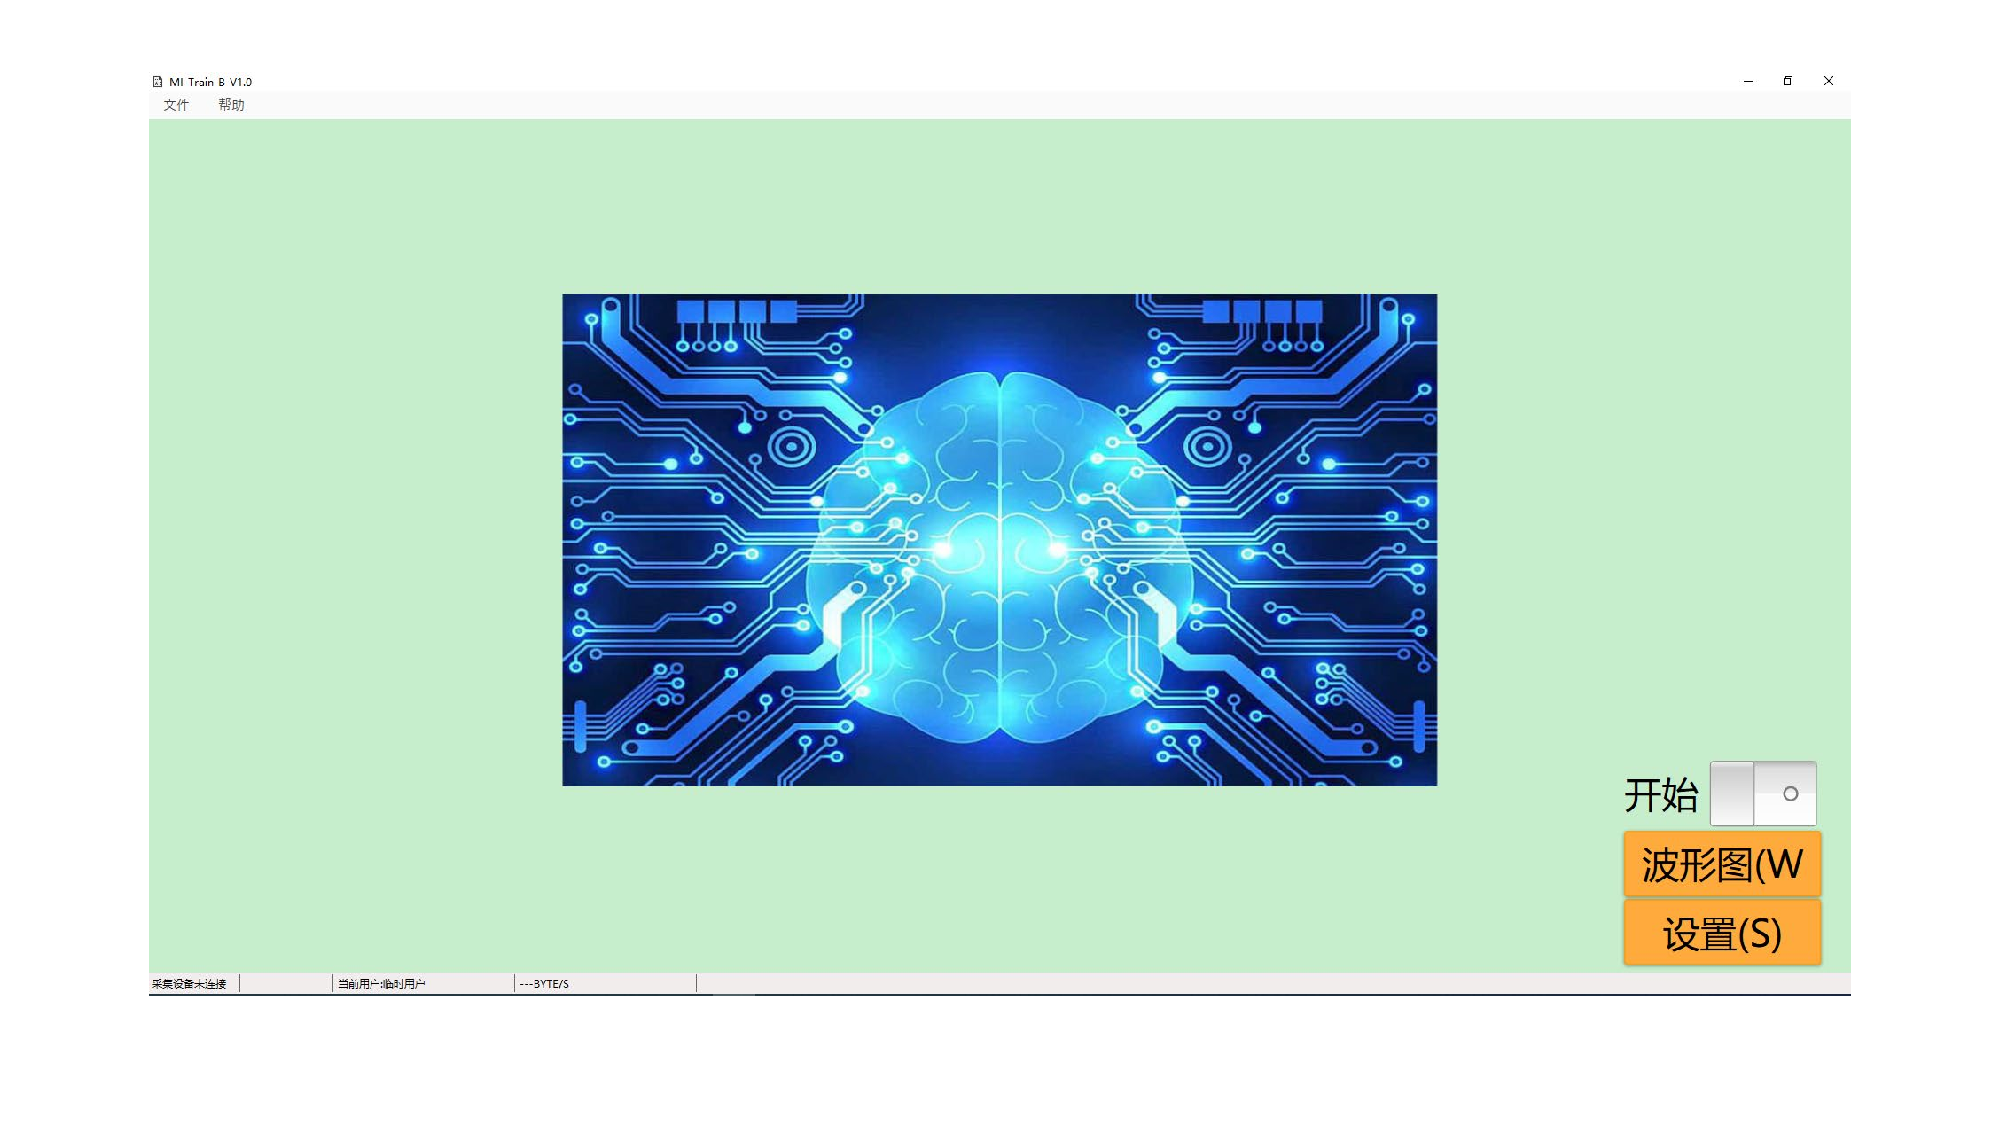
\includegraphics[width=0.6\textheight]{软件界面.pdf}
	\caption{上位机主界面} 
	\label{fig2-20}
\end{figure}

(1) 点击右下角设置按钮,在串口设置中选取下位机设备的串口号,在存储设置中选取EEG数据的目标存储位置。

(2) 设置完成后,点击文件下拉菜单中的打开串口按钮。这时下位机会向上位机发送准备就绪/需要重启的字符,引导使用者进行操作。

(3) 当设备准备就绪后,主界面左下角会出现采集设备已连接的提示。使用者点击主界面的开始按钮,上位机就会向下位机发送启动命令,下位机拉高ADS1299的START引脚,开始数据采集。

(4) 接收到数据后,上位机首先通过CRC校验位检查数据完整性。如果校验正确,则继续接收数据。如果校验失败,则暂停采集并提示使用者数据出错。

(5) 采集过程中,可以选择开启波形图实时观察采集信号。采集过程中的波形图如图\ref{fig2-21}所示。

\begin{figure}[h]
	\centering
	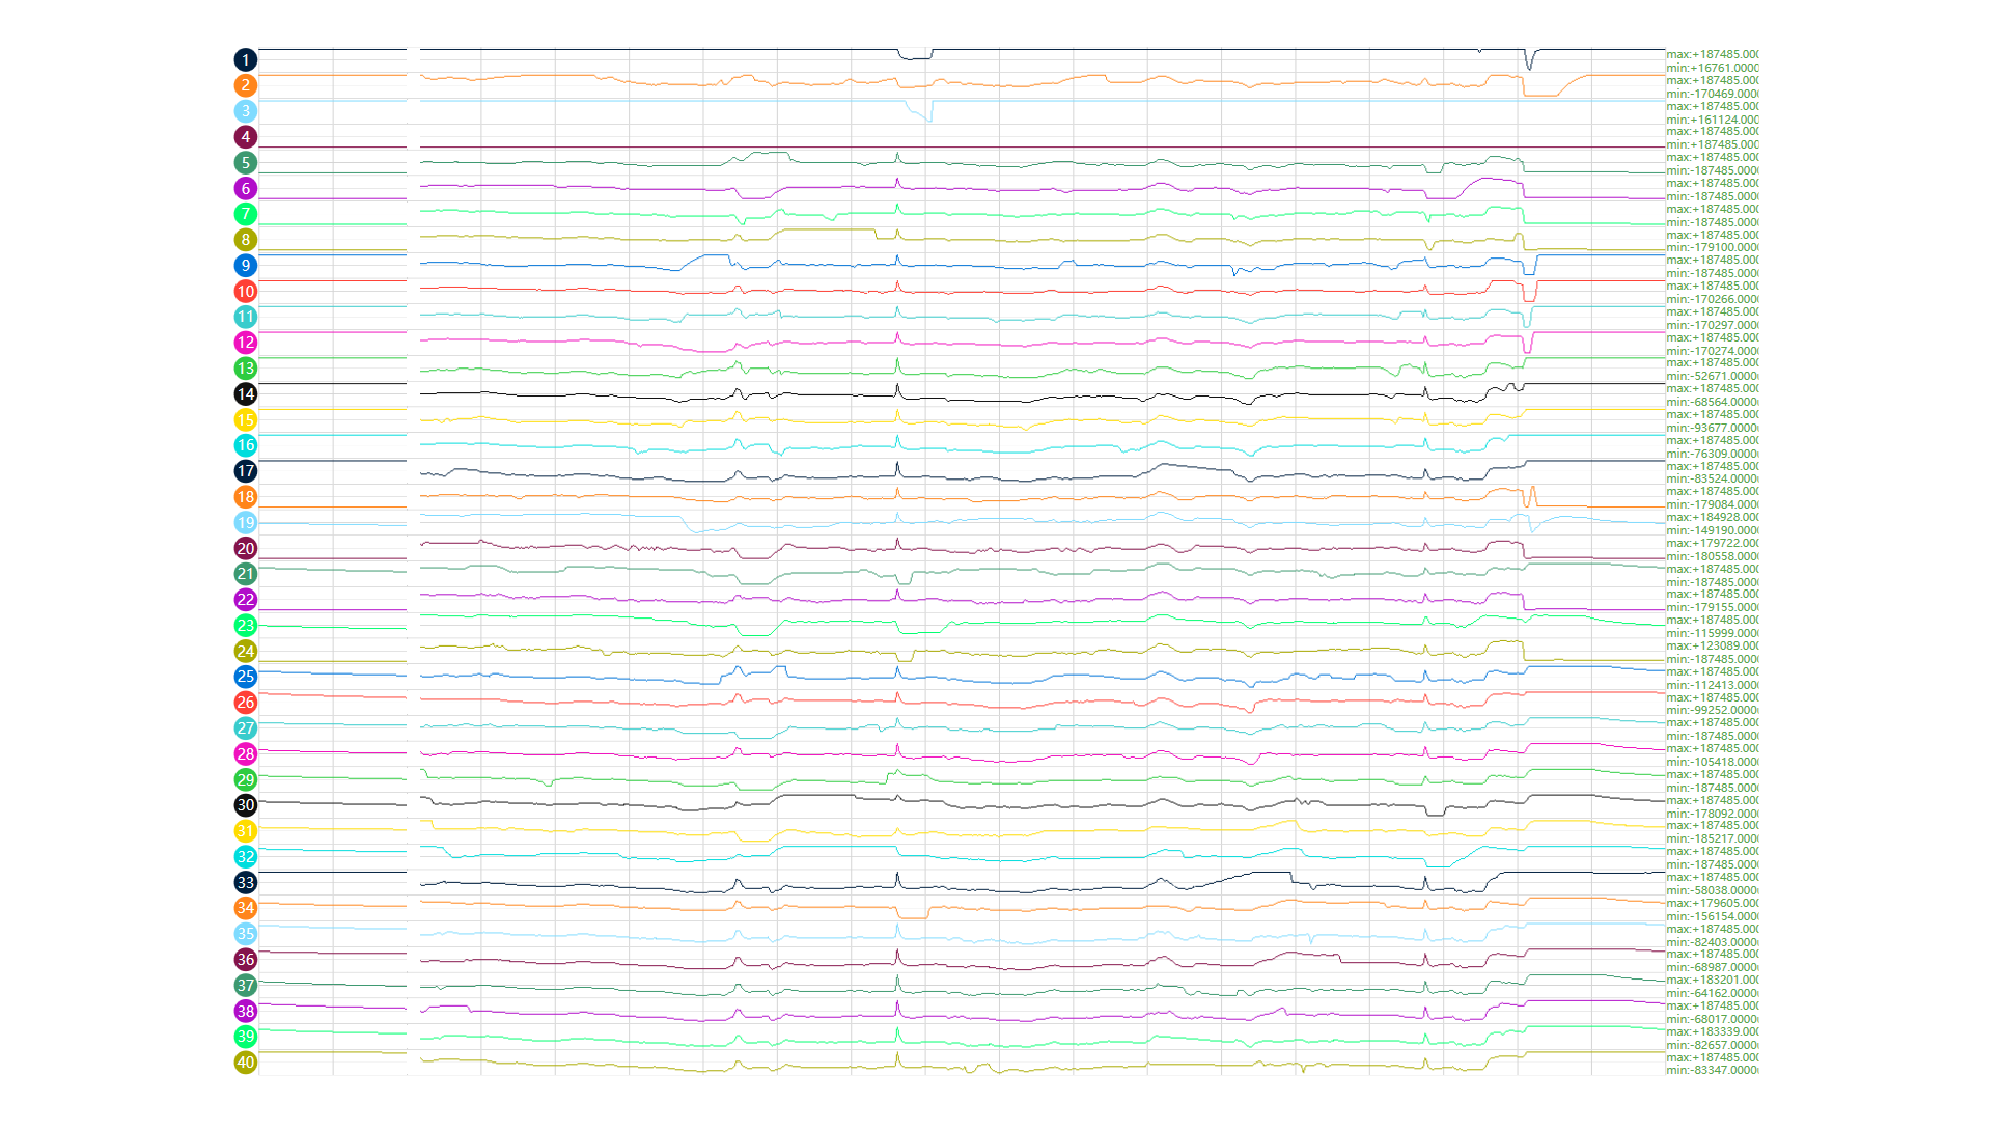
\includegraphics[width=0.52\textheight]{波形图界面.pdf}
	\caption{EEG波形图界面} 
	\label{fig2-21}
\end{figure}

(6) 采集结束后,关闭波形图界面,再次点击开始按钮,上位机会向下位机发送停止命令,下位机拉低ADS1299的START引脚,停止数据采集。

在给出具体需求和与下位机的通信方式后,上位机程序由深圳市缔峰泽公司实现编写。

\section{JS-AINS-40系统性能测试}
脑电采集设备在投入使用前需要经过严格的性能测试,以保证信号采集的准确有效。本节遵照中华人民共和国国家计量与检定规程JJG954-2019《数字脑电图仪》和中华人民共和国国家标准GB9706.226-2021《医用电气设备》中的步骤和要求进行性能检定。主要检定内容包括:电压测量、共模抑制比、噪声电平以及电磁兼容测试。

\subsection{电压测量}
电压测量遵循JJG954-2019《数字脑电图仪》中的要求,并使用SKX-8000微弱信号发生器来模拟检定仪与衰减器的输出。将不同幅值的0.1 s周期方波信号分别输入被检通道,记录30 s内波形幅值偏离最大者,并计算电压测量相对误差$\delta_{\mathrm{m}}$,其公式如下:
\begin{equation}
    \label{deqn_ex2_4}
    \delta_{\mathrm{m}}=\frac{U_{\mathrm{m}}-U_{\text {in }}}{U_{\text {m }}} \times 100 \%
\end{equation}

其中$U_{\mathrm{m}}$为偏离SKX-8000微弱信号发生器输入电压$U_{\text {in }}$的最大电压测量值。电压测量最大允许误差为$\pm 10 \times\left(1+\frac{U_1}{U_{\text {in}}}\right) \%$,其中$U_1$为设备当前灵敏度的五倍。JS-AINS-40系统的最高灵敏度为0.02 $\mu $V,考虑到JJG954-2019中要求的测试信号幅值远大于0.02 $\mu $V,这里直接使用$\pm 10\%$作为测量误差上界。

最终JS-AINS-40系统在不同输入电压下的测量相对误差如表\ref{tab2-2}所示。表中给出了每次测量所有通道中最大的相对误差值,可以看到,所有结果均在$\pm 10\%$以下,符合国标要求。

\begin{table}[!h]
	\centering
	\caption{电压测量相对误差}
	\wuhao{
			\begin{tabular}{cccccc}
			\toprule
			检定仪输出/  $\mu $V  & 相对误差   &检定仪输出/  $\mu $V  & 相对误差   &检定仪输出/  $\mu $V  & 相对误差   \\ 
			\midrule
			 10   & 9.2\%   &  50   & 5.9\%  &  500   &  0.9\%\\ 
			 20  & 7.4\%   &  100  & 3.5\%  &  1000  &  0.5\%\\ 
			 25  & 6.8\%   &  200  & 1.6\%  &  2000  &  0.4\%\\
			\bottomrule
		\end{tabular}
	}
	\label{tab2-2}
\end{table}

\subsection{共模抑制比}

基于前文所述,JS-AINS-40系统基于差模输入的方式采集EEG信号,而外部噪声基本以共模形式进入采集设备。因此,JS-AINS-40系统需要具备足够的共模抑制比来降低噪声对EEG信号的干扰。本节依然使用SKX-8000微弱信号发生器来模拟检定仪与衰减器的输出。遵照JJG954-2019,首先向JS-AINS-40系统输入50 Hz,幅值为200 $\mu$V的差模信号(JS-AINS-40系统的采集电极连接信号源正极,参考电极和右腿驱动电极连接信号源负极),记录差模信号幅值$U_d$。向JS-AINS-40系统输入50 Hz,幅值为2 V的共模信号(JS-AINS-40系统的采集电极和参考电极连接信号源正极,右腿驱动电极连接信号源负极),记录共模信号幅值$U_c$。按照公式\ref{deqn_ex2_5}计算所有通道的共模抑制比。

\begin{equation}
    \label{deqn_ex2_5}
    C M R R = 20 \lg K + 20 \lg\frac{U_{\mathrm{d}}}{U_{\mathrm{c}}}
\end{equation}

\begin{figure}[!h]
	\centering
	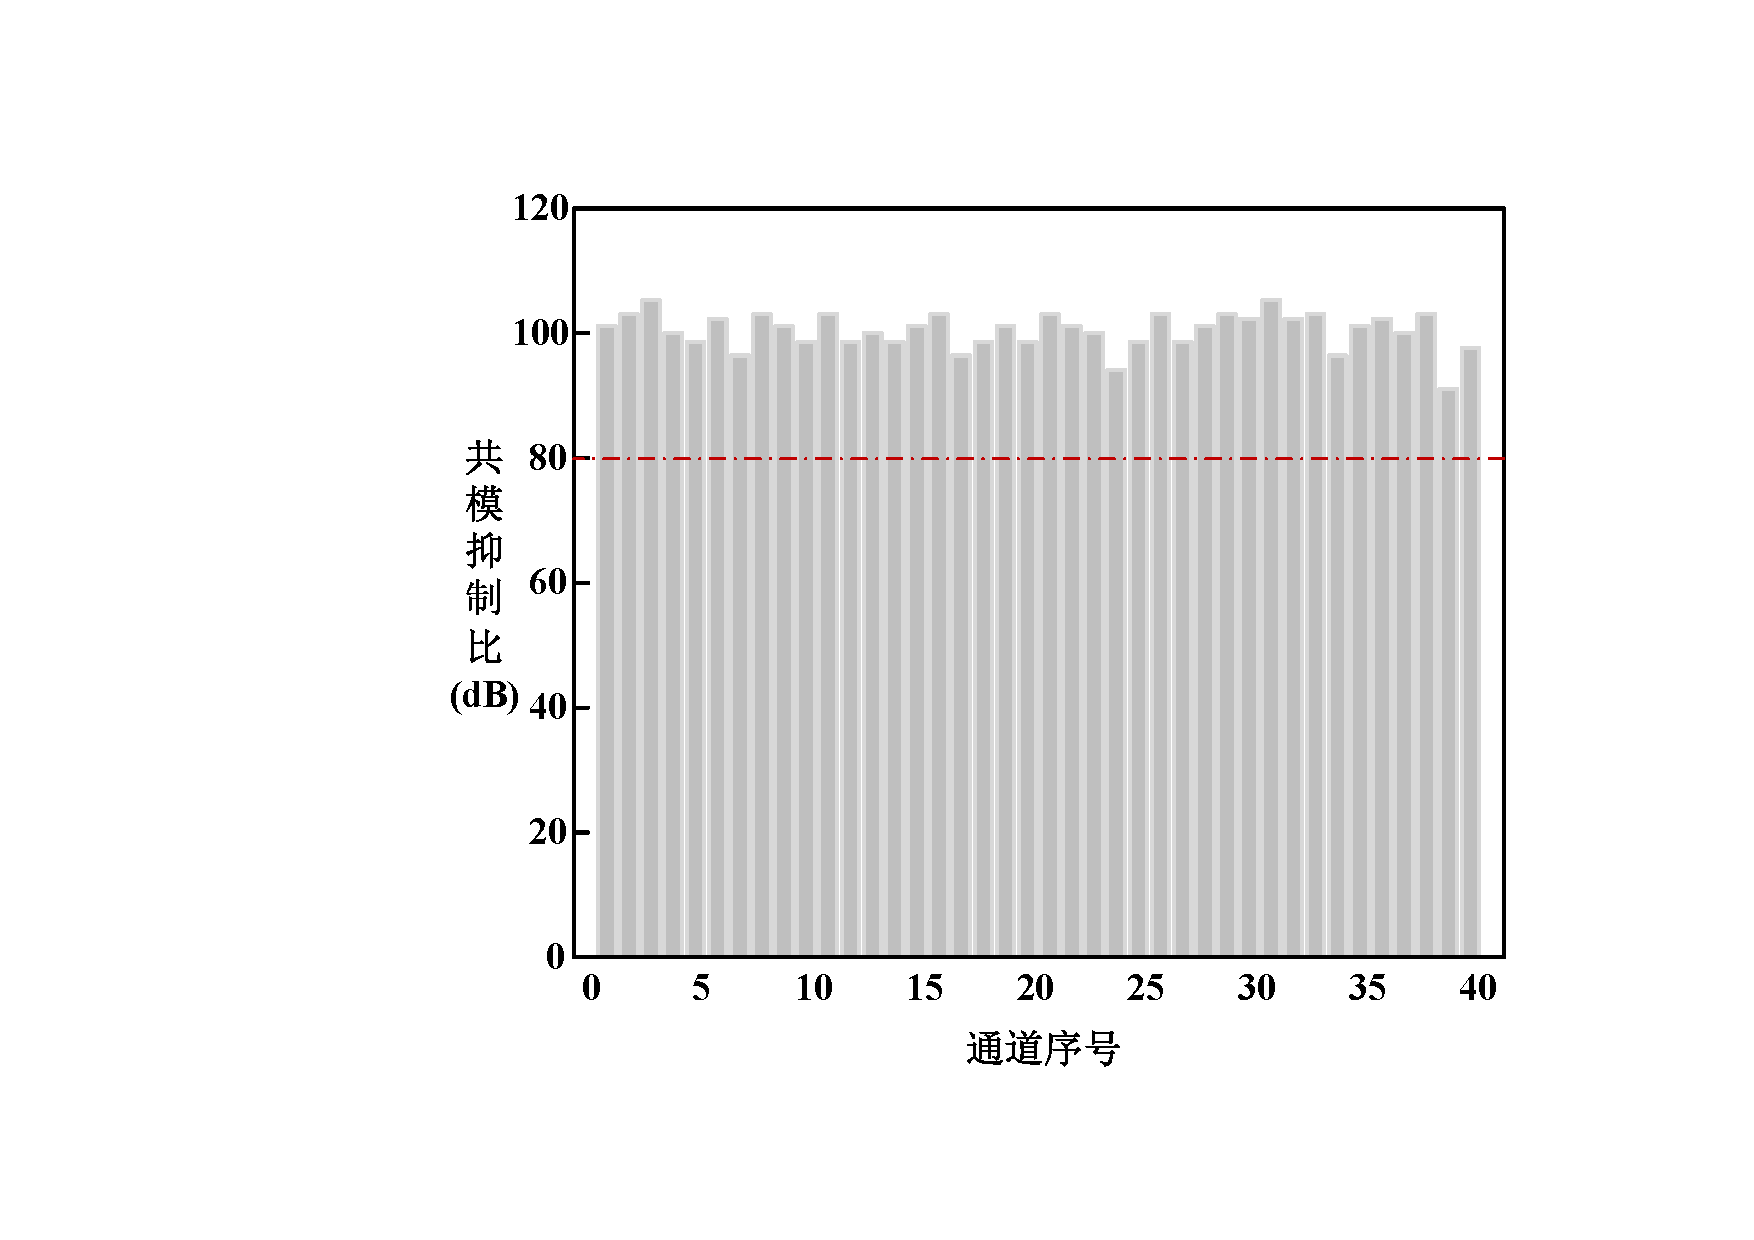
\includegraphics[width=0.37\textheight]{共模抑制比.pdf}
	\caption{通道的共模抑制比} 
	\label{fig2-23}
\end{figure}
其中$K$为SKX-8000输入的共模信号电压与差模信号电压比值。得到四十个通道的共模抑制比如图\ref{fig2-23}所示,可以看到,所有通道的共模抑制比均大于80 dB,符合国标要求。



\subsection{噪声电平}
JJG954-2019中对于噪声电平的定义为:采集设备的各通道输入端对地短接时,采集到的10 s噪声信号幅值。根据这一定义,本节将设备所有采集电极,参考电极和右腿驱动电极短接至屏蔽地,而后开始信号采集,并记录其幅度值。40个通道的噪声如图\ref{fig2-24}所示,可以看到所有通道噪声的最大幅值均在6 $\mu$V以内,符合GB9706.226-2021国标要求。
\begin{figure}[!h]
	\centering
	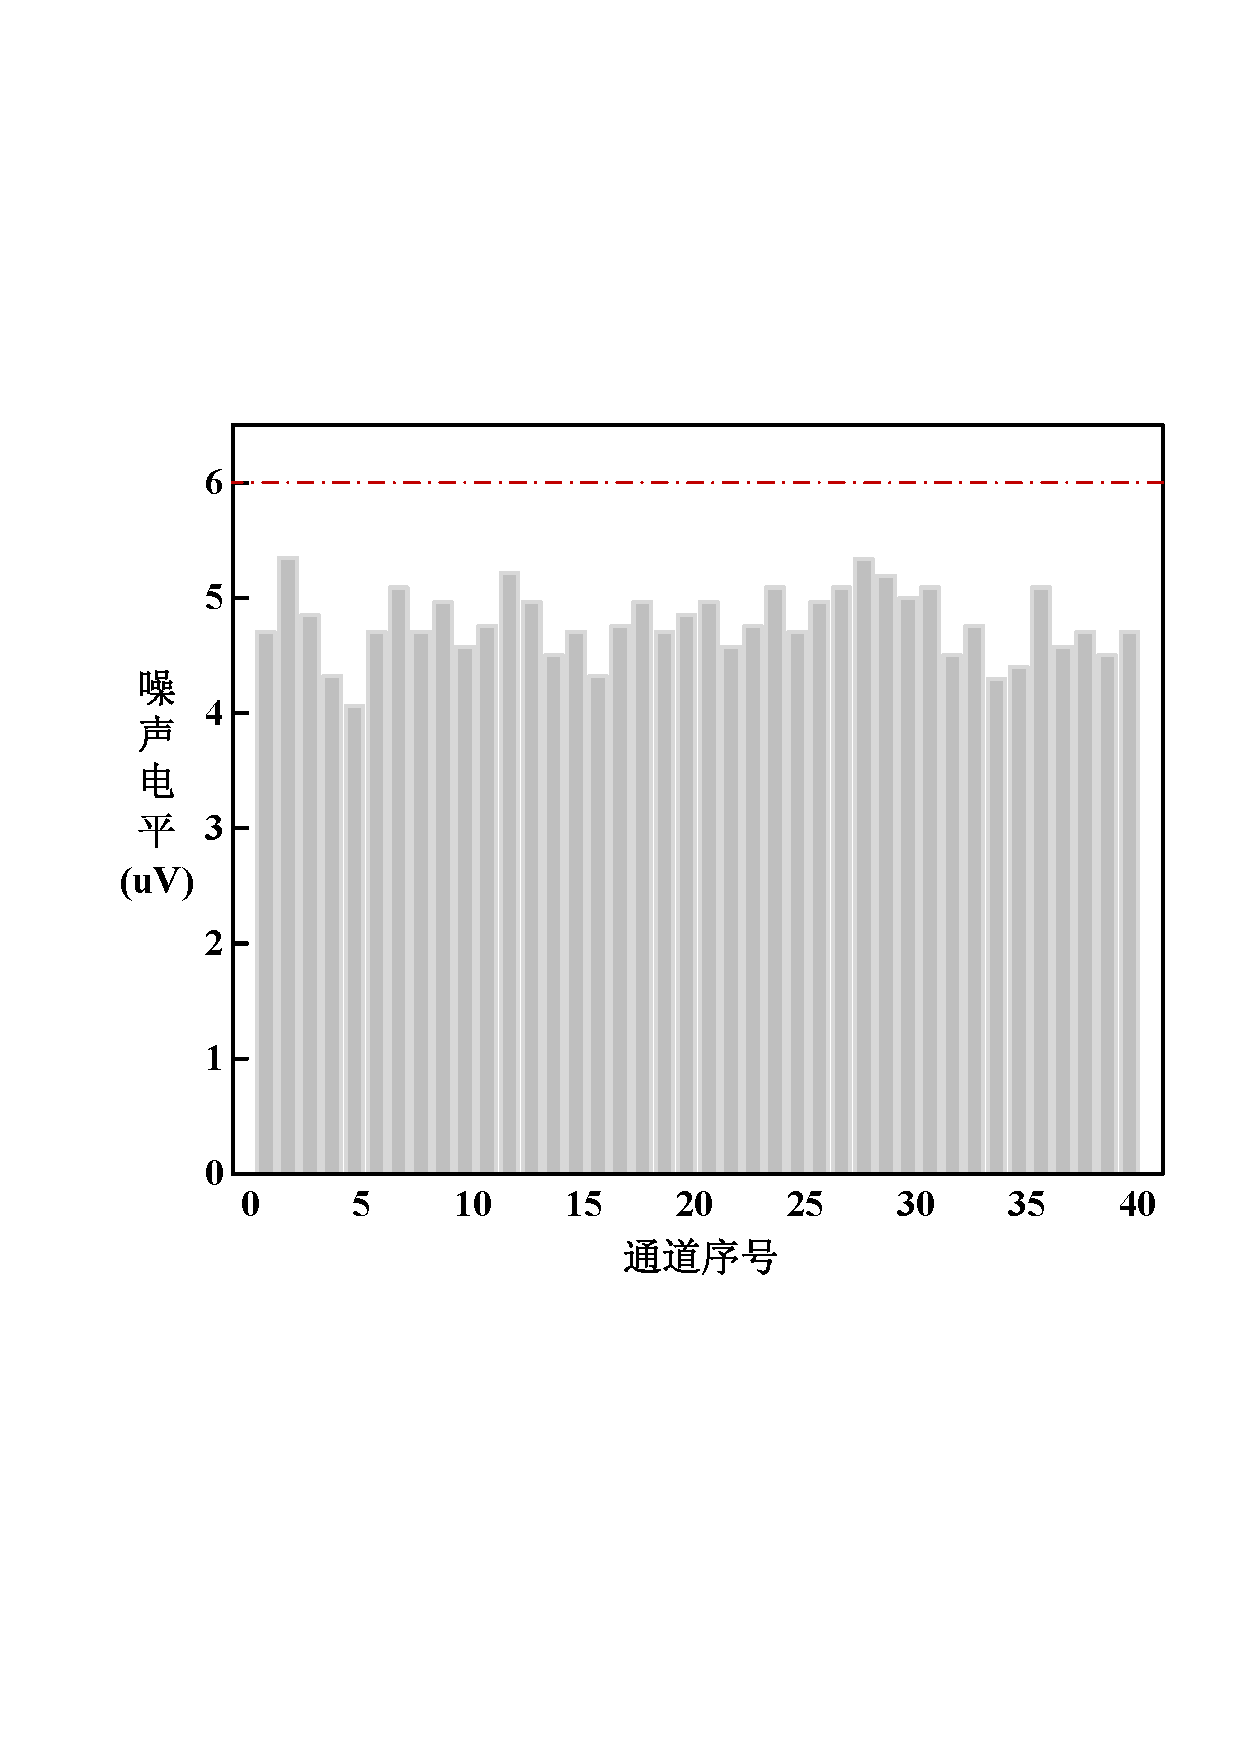
\includegraphics[width=0.37\textheight]{噪声.pdf}
	\caption{通道噪声电平} 
	\label{fig2-24}
\end{figure}

\subsection{电磁兼容测试}
JS-AINS-40系统作为一种电子设备,其需要在常规电磁环境中正常运行,并且不能对其他电子产品造成无法忍受的电磁干扰。因此,本节对其进行了电磁兼容测试(Electro Magnetic Compatibility,EMC)。进行的测试包括:静电测试、辐射发射测试以及射频场感应的传导骚扰抗扰度测试。静电测试和传导抗扰度测试的现场如图\ref{fig2-25}所示。

\begin{figure}[!h]
	\centering
	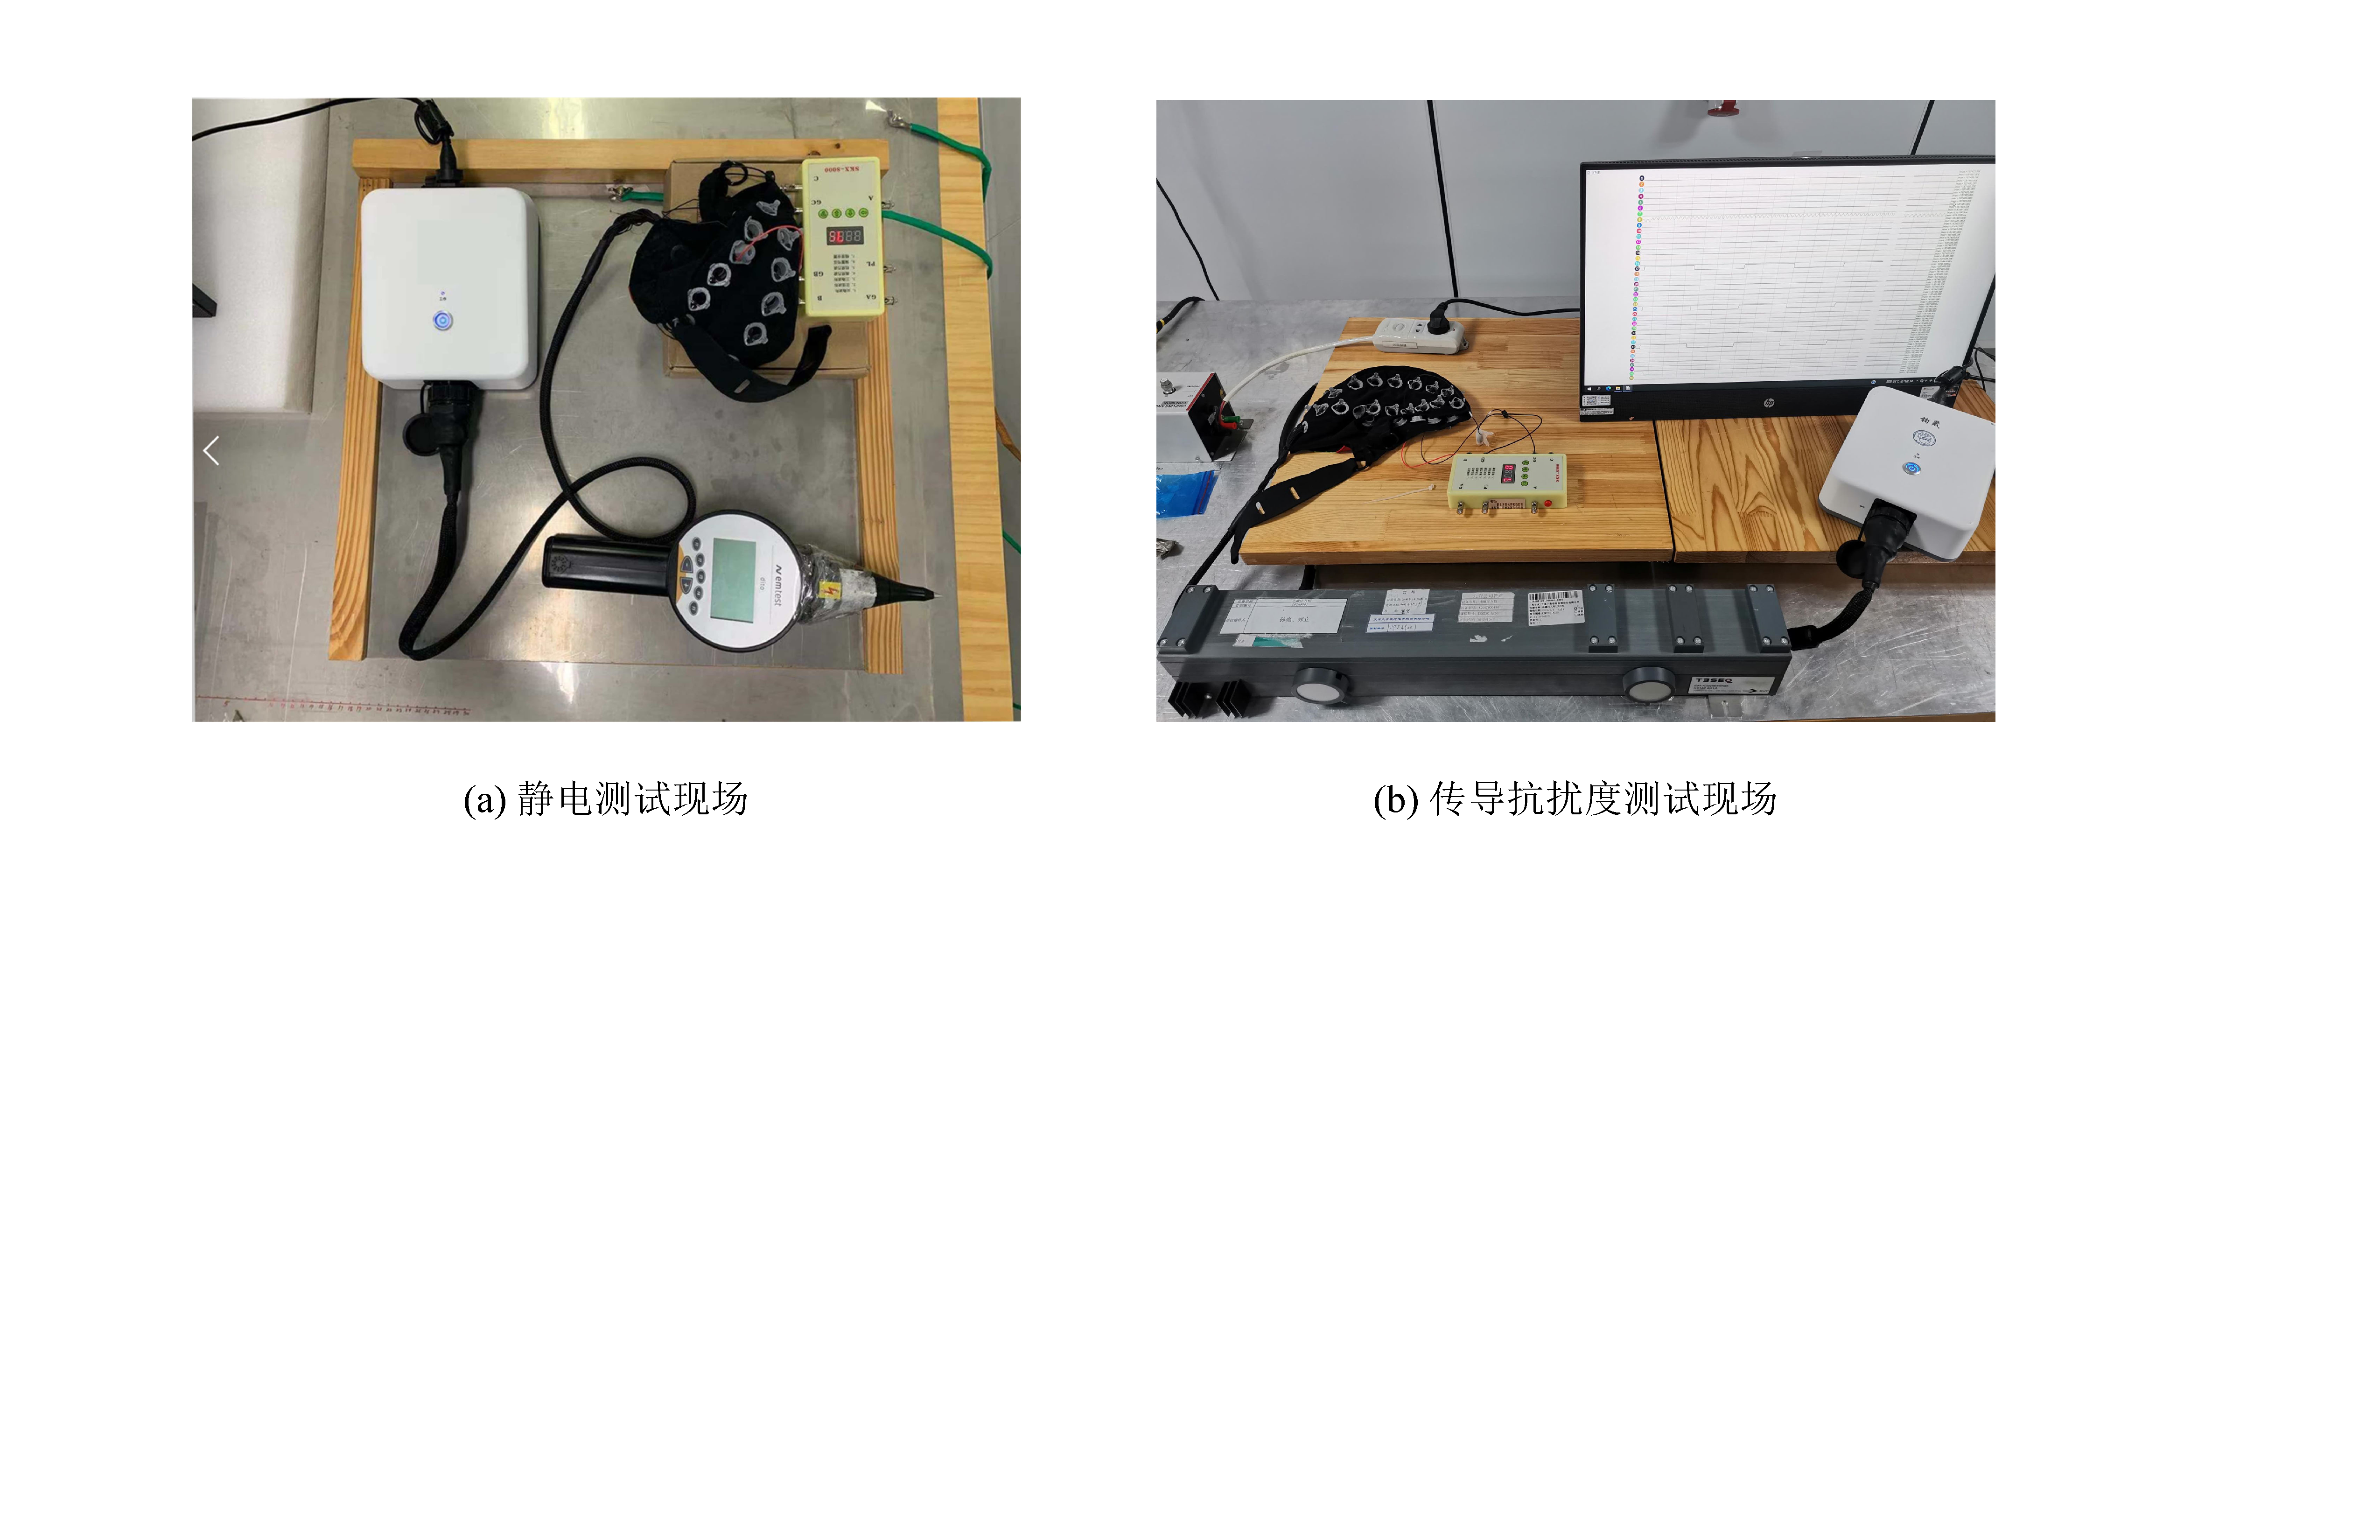
\includegraphics[width=0.60\textheight]{EMC.pdf}
	\caption{EMC测试现场} 
	\label{fig2-25}
\end{figure}

在测试中,JS-AINS-40系统能够承受8 kV的空气放电和6 kV的接触放电,符合静电测试要求;同时,JS-AINS-40系统在150 kHz至80 MHz的频率范围内,能够承受3类实验等级的射频发射机传导线电磁骚扰,符合国标要求的医疗设备抗扰度要求。


\begin{figure}[!h]
	\centering
	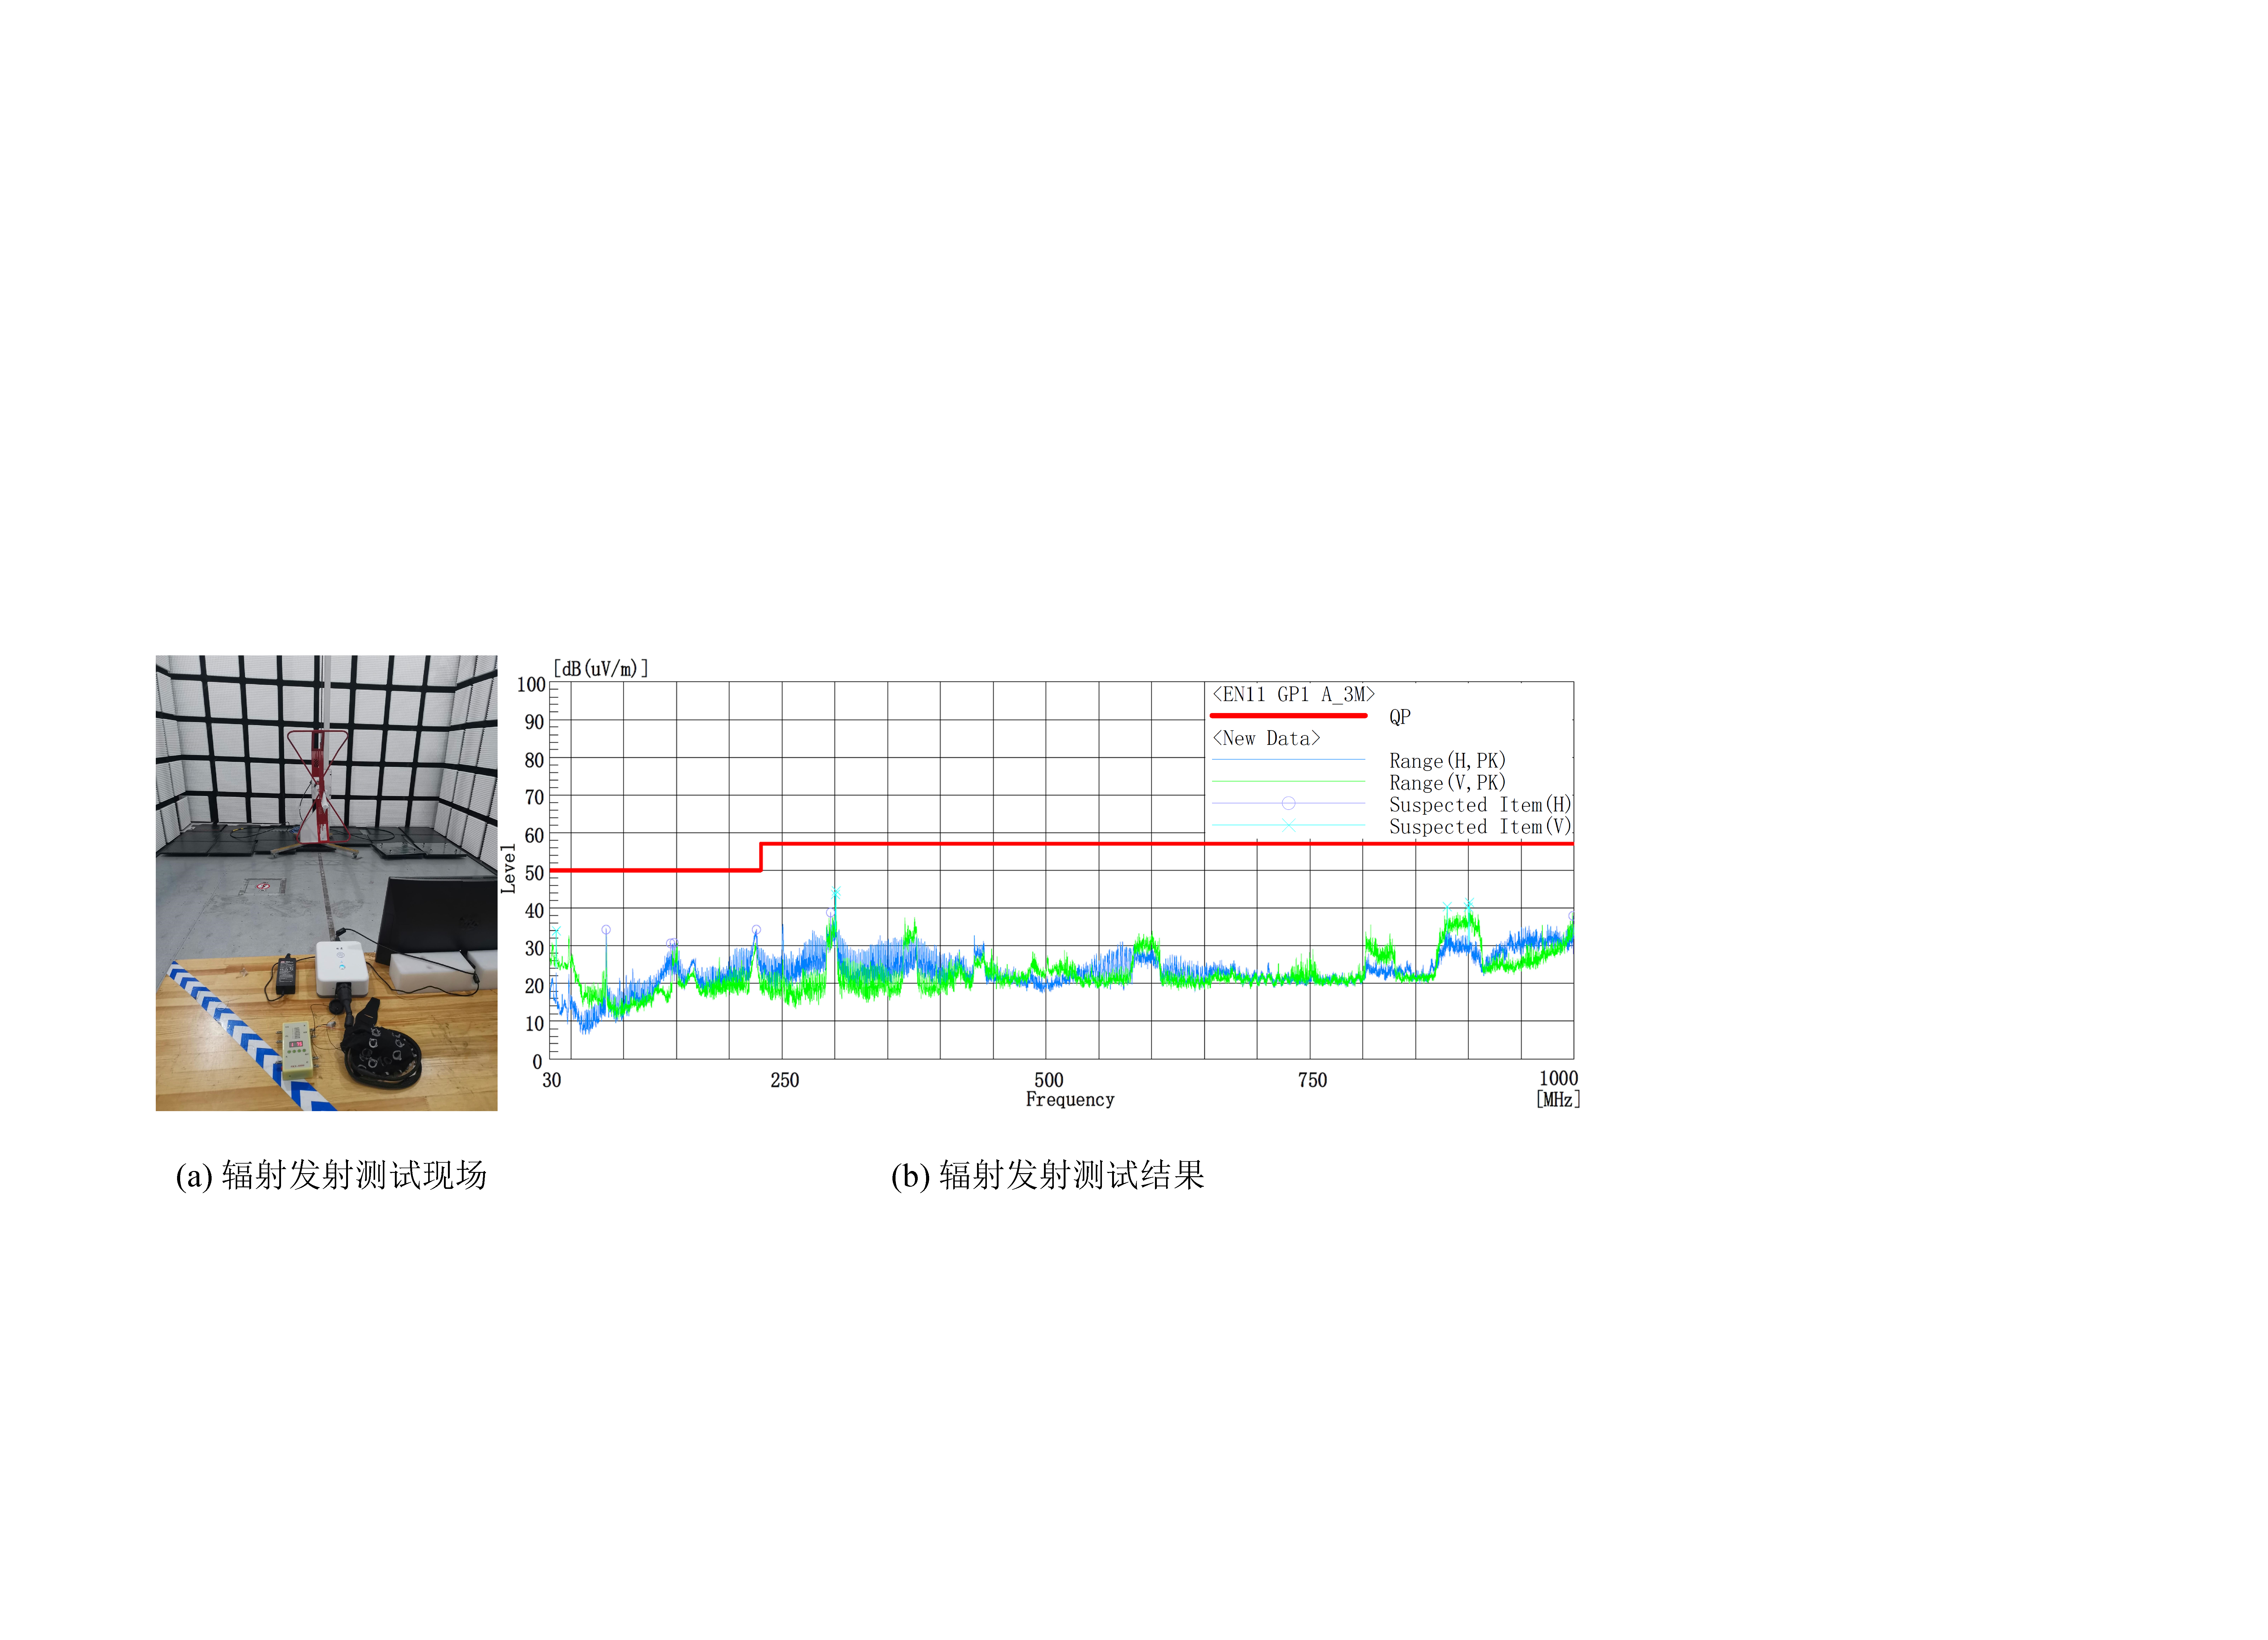
\includegraphics[width=0.60\textheight]{re_3.pdf}
	\caption{辐射发射测试现场与测试结果} 
	\label{fig2-26}
\end{figure}

辐射发射测试检测了JS-AINS-40系统在30 MHz-100 MHz频段内对外界的辐射干扰强度,检测现场及结果如图\ref{fig2-26}。图\ref{fig2-26}(b)中的红线代表国标设定的最大辐射干扰强度,可以看到,JS-AINS-40系统远低于这一指标,符合医疗电气设备的EMC要求。


\section{本章小结}
本章引入了自主设计的40导联EEG采集系统——JS-AINS-40,并以此为核心展开了详细介绍。首先,本章阐述了EEG信号的主要特点,并说明了针对这些特点,EEG采集设备应当具有的具体性能指标。紧接着,本章介绍了JS-AINS-40系统的整体框架——上位机、受试者和采集模块。其中作为核心的采集模块内部包含:虚拟串口通讯模块、数字电源模块、STM32H743IIT6主控模块、SPI隔离模块、电源隔离模块、ADS1299采集模块、模拟电源模块、采集前端与右腿驱动模块以及脑电极帽。考虑到实际使用时的安全性和可靠性,本章将上述子模块的电路集成在了脑电采集盒中,整个采集模块重量轻,体积较小,使用较为方便。接下来,本章说明了采集模块各子模块的器件选型以及配套电路,完成了对于JS-AINS-40系统硬件部分的介绍。

对于JS-AINS-40系统的软件部分,本章围绕下位机软件设计和上位机软件设计分别展开。其中下位机软件配合采集模块的硬件进行设计,使用STM32H743IIT6单片机控制ADS1299采集芯片,实现原始EEG数据的采集,并将其发送给上位机。上位机软件通过虚拟串口与下位机进行通信,并将接收的原始EEG数据进行存储与可视化。

最后,对JS-AINS-40系统的性能进行了测试与分析,从电压测量、共模抑制、噪声电平和EMC测试的结果可以看出,JS-AINS-40系统符合国标的相关要求,能够胜任EEG采集任务。接下来的章节,将使用JS-AINS-40系统采集相关EEG数据,并利用所提出的辨识算法对其进行分析。





